\documentclass[11pt]{memoir}
\usepackage{fontspec}
\defaultfontfeatures{Ligatures=TeX} 
\setmainfont{Gentium Book Basic} % or any font on your system
\setsansfont{Lucida Sans Unicode} % or any font on your system
%
\usepackage[top=20mm,bottom=20mm,left=25mm,right=25mm]{geometry}
\usepackage{microtype,soul,filecontents,pifont}
\usepackage{amsmath,etoolbox}
\usepackage{tikz}
\usetikzlibrary{decorations.markings}
%\usepackage{doc}
\usetikzlibrary{calc} 
\usetikzlibrary{decorations,decorations.shapes,shapes}
\usepackage{lettrine,caption,multicol}
\usepackage{xcolor}
\usepackage{lipsum,soul}
%\usepackage{palatino}
\usepackage{calligra}
\usepackage{fourier-orns}
%\usepackage[T1]{fontenc}

\usepackage{eso-pic}
\usepackage{layouts}
\usepackage{alphalph}
\usepackage{caption}
\usepackage{fmtcount}
\makeatletter
\usepackage[listings,theorems]{tcolorbox}
%\usepackage[charter]{mathdesign}
% \def\rmdefault{bch} % not scaled
% \def\ttdefault{blg}
\usepackage{xcolor,filecontents,ragged2e}
\definecolor{theblue} {rgb}{0.02,0.04,0.48}
\definecolor{thered}  {rgb}{0.65,0.04,0.07}
\definecolor{thegreen}{rgb}{0.06,0.44,0.08}
\definecolor{thelightgreen}{rgb}{0.06,0.44,0.06}
\definecolor{thegrey} {gray}{0.5}
\definecolor{thegray} {gray}{0.5}
\definecolor{thedarkgray} {gray}{0.95}
\definecolor{theshade}{gray}{0.94}
\definecolor{theframe}{gray}{0.75}
\definecolor{thecream}{rgb}{1,0.95,0.4}
\definecolor{spot}{rgb}{0,0.2,0.6}
\definecolor{boxframe}{gray}{0.8}
\definecolor{boxfill}{rgb}{0.95,0.95,0.99}
\definecolor{theoption}{rgb}{0.118,0.546,0.222}
\definecolor{themacro}{rgb}{0.784,0.06,0.176}
\definecolor{ExampleFrame}{rgb}{0.628,0.705,0.942}
\definecolor{ExampleBack}{rgb}{0.963,0.971,0.994}
\definecolor{Hyperlink}{rgb}{0.281,0.275,0.485}
\colorlet{thehyperlink}{theblue}
\newcommand*{\defaultcolor}{\color{black}}
\newcommand*{\spotcolor}{\color{spot}}

\newcommand\lorem{Fusce adipiscing justo nec ante. Nullam in enim.
 Pellentesque felis orci, sagittis ac, malesuada et, facilisis in,
 ligula. Nunc non magna sit amet mi aliquam dictum. In mi. Curabitur
 sollicitudin justo sed quam et quadd. \par}
%http://tex.stackexchange.com/questions/41150/background-baseline-grid-with-output-routine

\iffalse
\AddToShipoutPicture{%
    \begin{tikzpicture}[overlay,remember picture]
        \draw[thick,red]
              (current page.north east)
              rectangle (current page.south west);
        \draw[red!30!white,thin]
             (current page.south west) grid[step=2mm]
             (current page.north east);
        \draw[red!30!white,dotted]
             (current page.south west) grid[step=1cm]
             (current page.north east);
    \end{tikzpicture}%
}
\fi

\lstloadlanguages{[LaTeX]TeX, [primitive]TeX}

% Emphasis
\newcommand\emphasis[2][thered]{\lstset{emph={newcommand,def,gdef,#2},
   emphstyle={\bfseries\ttfamily\textcolor{#1}}}}%

\lstset{language={[LaTeX]TeX},
      escapeinside={{(*@}{@*)}}, 
       numbers=left, gobble=0,
       stepnumber=1,numbersep=5pt, 
       numberstyle={\footnotesize\color{gray}},firstnumber=10,
       breaklines=true,
       framesep=5pt,
       basicstyle=\small\ttfamily,
       showstringspaces=false,
      keywordstyle=\bfseries\ttfamily\textcolor{thegreen},
      stringstyle=\color{orange},
      commentstyle=\color{black},
      rulecolor=\color{theshade},
      breakatwhitespace=true,
     showspaces=false,  % shows spacing symbol
      xleftmargin=0pt,
      xrightmargin=5pt,
      aboveskip=3pt plus1pt minus1pt, % compact the code looks ugly in type
      belowskip=7pt plus1pt minus1pt,  % user responsible to insert any skips
      backgroundcolor=\color{theshade}
}

\graphicspath{{chapters/}}

\begin{filecontents*}{chapterx.sty}
\ProvidesPackage{chaptersx}[2012/04/07 v0.1 Typesetting chapters]
\def\HUGE{\@setfontsize\Huge{38}{47}}
\def\HHUGE{\@setfontsize\HHUGE{58}{67}}

\def\@words@cx#1{%
  \ifcase#1 zero\or one\or two\or three\or four\or five\or six\or seven\or eight\or nine\or ten\or
   eleven\or twelve\or thirteen\or fourteen\or fifteen\or sixteen\or seventeen\or eighteen\or nineteen \or twenty\or twenty one\or twenty two\or twenty three\or twenty four\or twenty five\or twenty six\or twenty seven \or twenty eight \or twenty nine\or thirty\or thirty one\or thirty two\or thirty three\or thirty four\or thirty five\or thirty six\or thirty seven\or thirty eight\or thirty nine\or forty\or forty one\or forty two \or forty three\or forty four\or forty five \or forty six \or forty seven\or forty eight \or forty nine\or fifty\or fifty on\or fifty two\or fifty three\or fifty four\or fifty five\or fifty six\or fifty seven\or fifty eight\or fifty nine\or sixty \or sixty one \or sixty two
\or sixty three \or sixty four \or \sixty five\else\@ctrerr\fi}



\newenvironment{absquote}
               {\list{}{\leftmargin2cm\rightmargin\leftmargin}%
                \item\relax\footnotesize}
               {\endlist}

\newenvironment{summary}
               {\list{}{\listparindent0pt %
                        \itemindent\listparindent
                        \leftmargin0pt
                        \rightmargin\leftmargin
                        \parsep\z@ \@plus\p@}%
                \item\relax\itshape}
               {\endlist}

% helper macros
\gdef\thinrule{\rule{\textwidth}{0.4pt}}
\gdef\mediumrule{\rule{\textwidth}{0.8pt}}
%% broad positions
\newif\if@left
\newif\if@right
\newif\if@center
\@leftfalse
\@rightfalse
\@centerfalse
% newifs for number position
\newif\if@lefttitle
\newif\if@righttitle
\newif\if@leftname
\newif\if@rightname
\newif\if@chapterspaceout\@chapterspaceoutfalse
\newif\if@titlespaceout\@chapterspaceoutfalse
\newif\if@sectionspaceout\@sectionspaceoutfalse
\newif\if@openanywhere\@openanywherefalse
%% The chapter command does not allow for openleft pages which we need
%% for some of the designs. 
\newif\if@openleft\@openleftfalse
\newif\if@openany\@openanyfalse

\newif\if@toc  \@toctrue
\newif\if@tocimage \@tocimagefalse
%\section{Libraries} 

\def\cx@optionlist{}


\def\cx@optionlist{}

\def\cxuselibrary#1{\cxset{library/.cd,#1}}
%
% The library is added by inputting the file and setting the path accordingly.
\def\cx@add@library#1#2{%
  \cxset{library/#1/.code={\@ifundefined{cxlibrary@#1@loaded}{\input #2}{}}}%
  \DeclareOption{#1}{\edef\cx@optionlist{\cx@optionlist,#1}}%
}

\def\thickrule{\leavevmode \leaders \hrule height 3pt \hfill \kern \z@}


% Define a family for chapter styling keys
\pgfkeys{/chapter/.is family}



\def\cxset{\pgfqkeys{/chapter}} %Notice this is pgf q keys
% spent half the evening to debug it;)Aarg!!!
% We define keys for all major components

\cxset{%
  name/.code={\gdef\chaptername{#1}},
  color/.store in=\color@cx,
  color/.default=black,
  chapter opening/.is choice,
  chapter opening/right/.code={\@openrighttrue},
  chapter opening/left/.code={\@openlefttrue},
  chapter opening/any/.code={\@openanytrue},
  chapter opening/none/.code={\@openanywheretrue\@openrightfalse
\@openleftfalse\@openanyfalse},
  chapter opening/anywhere/.code={\@openanywheretrue\@openrightfalse
\@openleftfalse\@openanyfalse},
  chapter opening/ifafter/.code={},
  chapter font-family/.store in=\chapterfontfamily@cx,
  chapter font-weight/.store in=\chapterfontweight@cx,
  chapter font-size/.store in=\chapterfontsize@cx,
  chapter color/.store in=\chaptercolor@cx,
  chapter before/.store in=\chapterbefore@cx,
  chapter after/.store in=\chapterafter@cx,
  chapter spaceout/.is choice,
  chapter spaceout/soul/.code={\@chapterspaceouttrue},
  chapter spaceout/none/.code={\@chapterspaceoutfalse},
  % title keys
  title font-family/.store in=\titlefontfamily@cx,
  title font-family/.default=\rmfamily,
  title font-weight/.store in=\titlefontweight@cx,
  title font-size/.store in=\titlefontsize@cx,
  title font-color/.store in=\titlefontcolor@cx,
  title font-shape/.store in= \titlefontshape@cx,
  title spaceout/.is choice,
  title spaceout/soul/.code={\@titlespaceouttrue},
  title spaceout/none/.code={\@titlespaceoutfalse},
  title font/.style={title font-family=#1},
  title before/.store in=\titlebefore@cx,
  title after/.store in=\titleafter@cx,
  title beforeskip/.store in=\titlebeforeskip@cx,
  title afterskip/.store in=\titleafterskip@cx,
  position/.is choice,
  position/left/.code={\@lefttrue},
  position/right/.code={\@righttrue},
  position/center/.code={\@centertrue},
% numbering options that are required
  numbering/.is choice,
% better to rename thechapter?
  numbering/roman/.code={\gdef\thechapter{\@roman\c@chapter}},
  numbering/Roman/.code={\gdef\thechapter{\@Roman\c@chapter}},
  numbering/arabic/.code={\gdef\thechapter{\@arabic\c@chapter}},
  numbering/alpha/.code={\gdef\thechapter{\alphalph\c@chapter}},
  numbering/Alpha/.code={\gdef\thechapter{\AlphAlph\c@chapter}},
  numbering/words/.code={\gdef\thechapter{\MakeTextLowercase{\expandafter\@words@cx{\expandafter\@arabic\c@chapter}}}},
%% These proved a bit trouble some and ended up calling the fmtcount package routines
  numbering/WORDS/.code={\gdef\thechapter{\NUMBERstring{chapter}}},
  numbering/Words/.code={\gdef\thechapter{\NumToName{\expandafter\@arabic\c@chapter}}},
%% These is for my own use for EJD type numbering, placed in an mbox as there is something funny
% happening with spaces.
  numbering/padzeroes/.code={\gdef\thechapter{\mbox{EWD -\padzeroes[4]\decimal{chapter}}%
  }%
 },
  numbering/none/.code={},
  number dot/.store in=\numberpunctuation@cx,
  number position/.is choice,
  number position/leftname/.code={\@leftnametrue\@rightnamefalse},
  number position/rightname/.code={\@rightnametrue\@leftnamefalse},
  number position/absolute/.code={},
  number position/righttitle/.code={\@righttitletrue},
  number position/lefttitle/.code={\@lefttitletrue},
  number after/.store in=\numberafter@cx,
  number before/.store in=\numberbefore@cx,
  number color/.store in=\numbercolor@cx,
  number font-size/.store in=\numberfontsize@cx,
  number font-family/.store in=\numberfontfamily@cx,
  number font-weight/.store in=\numberfontweight@cx,
  chapter toc/.is choice,
  chapter toc/true/.code=\@toctrue\cxset{numbering=arabic,name=Chapter},
  chapter toc/false/.code=\@tocfalse,
  chapter toc/none/.code=\@tocfalse,
% sectioning commands
  section font-size/.store in=\sectionfontsize@cx,
  section font-weight/.store in=\sectionfontweight@cx,
  section font-family/.store in=\sectionfontfamily@cx,
  section font-shape/.store in=\sectionfontshape@cx,
  section color/.store in=\sectioncolor@cx,
  section numbering/.is choice,
  section numbering/roman/.code={\gdef\thesection{\thechapter\@roman\c@section}\renewsection},
  section numbering/(roman)/.code={\gdef\thesection{\thechapter(\@roman\c@section)}\renewsection},
  section numbering/arabic/.code={\gdef\thesection{\thechapter.\@arabic\c@section}\renewsection},
  section numbering/numeric/.code={\gdef\thesection{\thechapter.\@arabic\c@section}\renewsection},
  section numbering custom/.code=\gdef\thesection{#1}\renewsection,
  section numbering/none/.code={\gdef\thesection{}\renewsection},
  section align/.store in=\sectionalign@cx,
  section beforeskip/.store in=\sectionbeforeskip@cx,
  section afterskip/.store in=\sectionafterskip@cx,
  section indent/.store in=\sectionindent@cx,
  section spaceout/.is choice,
  section spaceout/soul/.code={\@sectionspaceouttrue},
  section spaceout/none/.code={\@sectionspaceoutfalse},
% subsections
  subsection font-size/.store in=\subsectionfontsize@cx,
  subsection font-weight/.store in=\subsectionfontweight@cx,
  subsection font-family/.store in=\subsectionfontfamily@cx,
  subsection font-shape/.store in=\subsectionfontshape@cx,
  subsection color/.store in=\subsectioncolor@cx,
  subsection numbering/.is choice,
  subsection numbering/arabic/.code={\gdef\thesubsection{\thesection.\@arabic\c@subsection}},
  subsection numbering/custom/.store in=\thesubsection@cx,
  subsection numbering/none/.code={\gdef\thesubsection{}},
  subsection align/.store in=\subsectionalign@cx,
  subsection beforeskip/.store in=\subsectionbeforeskip@cx,
  subsection afterskip/.store in=\subsectionafterskip@cx,
  subsection indent/.store in=\subsectionindent@cx,
%%
%% subsubsection
  subsubsection font-size/.store in=\subsubsectionfontsize@cx,
  subsubsection font-weight/.store in=\subsubsectionfontweight@cx,
  subsubsection font-family/.store in=\subsubsectionfontfamily@cx,
  subsubsection font-shape/.store in=\subsubsectionfontshape@cx,
  subsubsection color/.store in=\subsubsectioncolor@cx,
  subsubsection numbering/.is choice,
  subsubsection numbering/numeric/.code={\gdef\thesubsubsection{\thesubsection.\@arabic\c@subsubsection}},
  subsubsection numbering/custom/.store in=\thesubsubsection@cx,
  subsubsection numbering/none/.code={\gdef\thesubsubsection{}},
  subsubsection align/.store in=\subsubsectionalign@cx,
  subsubsection beforeskip/.store in=\subsubsectionbeforeskip@cx,
  subsubsection afterskip/.store in=\subsubsectionafterskip@cx,
  subsubsection indent/.store in=\subsubsectionindent@cx,
%
% paragraph
%
  paragraph font-size/.store in=\paragraphfontsize@cx,
  paragraph font-weight/.store in=\paragraphfontweight@cx,
  paragraph font-family/.store in=\paragraphfontfamily@cx,
  paragraph font-shape/.store in=\paragraphfontshape@cx,
  paragraph color/.store in=\paragraphcolor@cx,
  paragraph numbering/.is choice,
  paragraph numbering/numeric/.code={\gdef\theparagraph{\thesubsubsection.\@arabic\c@paragraph}},
  paragraph numbering/custom/.store in=\theparagraph@cx,
  paragraph numbering/none/.code={\gdef\theparagraph{}},
  paragraph align/.store in=\paragraphalign@cx,
  paragraph beforeskip/.store in=\paragraphbeforeskip@cx,
  paragraph afterskip/.store in=\paragraphafterskip@cx,
  paragraph indent/.store in=\paragraphindent@cx,
%% subparagraphs
%
  subparagraph font-size/.store in=\subparagraphfontsize@cx,
  subparagraph font-weight/.store in=\subparagraphfontweight@cx,
  subparagraph font-family/.store in=\subparagraphfontfamily@cx,
  subparagraph font-shape/.store in=\subparagraphfontshape@cx,
  subparagraph color/.store in=\subparagraphcolor@cx,
  subparagraph numbering/.is choice,
  subparagraph numbering/numeric/.code={\gdef\thesubparagraph{\theparagraph.\@arabic\c@subparagraph}},
  subparagraph numbering/arabic/.code={\gdef\thesubparagraph{\theparagraph.\@arabic\c@subparagraph}}
  subparagraph numbering/custom/.store in=\thesubparagraph@cx,
  subparagraph numbering/none/.code={\gdef\thesubparagraph{}},
  subparagraph align/.store in=\subparagraphalign@cx,
  subparagraph beforeskip/.store in=\subparagraphbeforeskip@cx,
  subparagraph afterskip/.store in=\subparagraphafterskip@cx,
  subparagraph indent/.store in=\subparagraphindent@cx,
  subparagraph number after/.estore in=\subparagraphnumberafter@cx,
  subparagraph number after/.default=,
  subparagraph number after/.initial=,
%
%% headers and footers
  header style/.store in=\headerstyle@cx,
% general draft rules
  rule /.is choice,
  rule on/.code={\gdef\rulewidth@cx{0.4pt}},
  rule off/.code={\gdef\rulewidth@cx{0pt}},
% headers and footers
  lhead/.code ={\lhead{#1}},
  rhead/.code={\rhead{#1}},
  chead/.code={\chead{#1}},
  lfoot/.code ={\lhead{#1}},
  cfoot/.code={\chead{#1}},
  rfoot/.code={\rhead{#1}},
  headrulewidth/.code={\renewcommand\headrulewidth{#1}},
  footrulewidth/.code={\renewcommand\footrulewidth{#1}},
}



%% Commands to renew sectioning, these unfortunately need to be 
%% called explicitly
\def\renewsection{%
\renewcommand\section{%
\@startsection{section}%
{1}%level
{\sectionindent@cx}%indent
{\sectionbeforeskip@cx}%
{\sectionafterskip@cx}%
{\sectionfontweight@cx\sectionfontfamily@cx\sectionfontsize@cx\sectionfontshape@cx\sectionalign@cx}%
}%
}

\def\renewsubsection{%
\renewcommand\subsection{%
 \@startsection{subsection}%
{2}%level
{\subsectionindent@cx}%indent
{\subsectionbeforeskip@cx}%
{\subsectionafterskip@cx}%
{\subsectionfontweight@cx\subsectionfontfamily@cx\subsectionfontshape@cx%
 \subsectionfontsize@cx\subsectionalign@cx}%
}%
}

\def\renewsubsubsection{%
\renewcommand\subsubsection{%
 \@startsection{subsubsection}%
{3}%level
{\subsubsectionindent@cx}%indent
{\subsubsectionbeforeskip@cx}%
{\subsubsectionafterskip@cx}%
{\subsubsectionfontweight@cx\subsubsectionfontfamily@cx%
\subsubsectionfontsize@cx\subsubsectionfontshape@cx\subsubsectionalign@cx}%
}}

\def\renewparagraph{%
\renewcommand\paragraph{%
 \@startsection{paragraph}%
{4}%level
{\paragraphindent@cx}%indent
{\paragraphbeforeskip@cx}%
{\paragraphafterskip@cx}%
{\paragraphfontweight@cx\paragraphfontfamily@cx%
\paragraphfontsize@cx\paragraphfontshape@cx\paragraphalign@cx}%
}}

\def\renewsubparagraph{%
\renewcommand\subparagraph{%
 \@startsection{subparagraph}%
{5}%level
{\subparagraphindent@cx}%indent
{\subparagraphbeforeskip@cx}%
{\subparagraphafterskip@cx}%
{\subparagraphfontweight@cx\subparagraphfontfamily@cx%
\subparagraphfontsize@cx\subparagraphfontshape@cx\subparagraphalign@cx}%
}%
\def\@seccntformat##1{\csname the##1\endcsname\subparagraphnumberafter@cx}%
}



\cxset{%
  lhead=left head text,
  chead=center text,
  rhead=right text,
  lfoot=left text,
  cfoot=center text,
  rfoot=right text,
  headrulewidth=2pt,
  footrulewidth=0.4pt,
  color=blue,
  position=center,
  name=chapteris,
  title font-family=\rmfamily,
  title font-weight=\bfseries,
  title font-size=\Huge,
  title font-color=\color{olive},
  numbering=arabic,
  number dot=,
  chapter font-family=\sffamily,
  chapter font-weight=\bfseries,
  chapter font-size=\Large,
  chapter color=gray,
  chapter before={\leavevmode\par\hfill},%need to correct for 0pt
  chapter after=\hfill\hfill,
  number position=rightname,
  number color=\color{gray},
  number after=\hspace{20pt},
  number before=\hspace*{20pt},
  number font-size=\huge,
  number font-family=\sffamily,
  number font-weight=\bfseries,
  number before=,
  number after=,
  title before=,
  title after=,
  title afterskip={\vskip50pt},
  title beforeskip={\vskip10pt},
  header style=fancy,
}



\gdef\setdefaults{%
\cxset{%
  lhead=left head text,
  chead=center text,
  rhead=right text,
  lfoot=left text,
  cfoot=center text,
  rfoot=right text,
name=CHAPTER,
title font-family=\rmfamily,
title font-weight=\bfseries,
title font-size=\Huge,
title font-color=\color{purple},
numbering=arabic,
number dot=,
number before=,
number after=,
chapter font-family=\sffamily,
chapter font-weight=\bfseries,
chapter font-size=\large,
chapter spaceout=soul,
chapter color=gray,
chapter before={},%need to correct for 0pt
chapter after=,
number position=rightname,
number color=\color{gray},
number after=\hspace{20pt},
number before=\space,
number font-size=\large,
number font-family=\sffamily,
number font-weight=\bfseries,
title before=,
title after=,
title afterskip={\vskip24pt},
title beforeskip={\vskip10pt},
title font=\rmfamily,
header style=plain,
section font-weight=\bfseries,
section font-family=\rmfamily,
section font-size=\Large,
section font-shape=\upshape,
section align=\raggedright,
title font-shape=\upshape,
}
}

%% STYLE 13
\cxset{style13/.style={
 name={Chapter},
 numbering=arabic,
 number font-size=\HUGE,
 number font-family=\sffamily,
 number font-weight=\bfseries,
 number color=\color{gray!50},
 number before=\par\vspace*{5pt}\hfill\hfill,
 number dot=,
 number after={\hspace*{7pt}\par},
 number position=rightname,
 chapter font-family=\sffamily,
 chapter font-weight=\normalfont,
 chapter font-size=\LARGE,
 chapter before={\thinrule\vspace*{20pt}\par\hfill\hfill},
 chapter after={\vskip0pt\par},
 chapter color={black!50},
 title beforeskip={\vspace*{10pt}},
 title afterskip={\vspace*{50pt}\par},
 title before={\hfill\hfill\raggedleft},
 title after={},
 title font-family=\sffamily,
 title font-color=\color{purple},
 title font-weight=\bfseries,
 title font-size=\huge,
 section indent=-1em,
 section align=\raggedright,
 section numbering=arabic,
 section indent=0pt,
 section beforeskip=0pt,
 section afterskip=\baselineskip,
 subsection align=\raggedright,
 subsection font-family=\sffamily,
 subsection font-weight=\bfseries,
 subsection font-size=\large,
 subsection font-shape=\itshape,
 subparagraph number after=\space,
}
}



% The |\@makechapterhead| is used by LaTeX to typeset the
% Chapter heading. This is a rewrite in order to make it
% more flexible and use the keys.
% #1 spare
% #2 title
\newif\if@special\@specialfalse
\cxset{custom/.code=\gdef\customdesign@cx{\csname#1\endcsname}\@specialtrue,
       fill/.store in=\fill@cx}
\cxset{custom=tikzspecial,
    title font-size=\Large,
    title font-color=\color{white},
    title font-family=\sffamily,
    fill=thegrey,
}

\renewcommand\@makechapterhead[2][]{%
% macro for typesetting the chapter number
\if@special
    \customdesign@cx{#2}
   \else
  \def\printnumber{%
    \numberbefore@cx
      {%
      \numbercolor@cx
      \numberfontsize@cx
      \numberfontfamily@cx
      \numberfontweight@cx
      \thechapter
      \numberpunctuation@cx
      }
      \numberafter@cx
  }%
% macro for typesetting the chapter name
  \def\printchaptername{%
    {
    \chapterfontfamily@cx
    \chapterfontsize@cx
    \chapterfontweight@cx
    \color{\chaptercolor@cx}
% Check if the chapter name is spaced out and use the
% soul package. TODO add values for soul parameters
% as a style feature.
    \if@chapterspaceout 
     \expandafter\so\expandafter{\chaptername}
    \else
      \@chapapp\space
    \fi
    }%
  }%
% set all keys
    {%
    \parindent0pt 
    \normalfont%
    \ifnum \c@secnumdepth>\m@ne%
      \if@mainmatter%
 % we start displaying  the names and any preambles such 
 % as images
 % print chapter name
         \chapterbefore@cx%
         \if@leftname
            \printnumber
         \fi%
         \printchaptername
         \if@rightname
            \printnumber
         \fi%
         \chapterafter@cx  
      \fi%
    \fi%
     %chapter title
    \interlinepenalty\@M%
% if the number is before the title
% if the number prints together with the title they 
% are considered as one indivisible part.
     \titlebeforeskip@cx%
     \if@lefttitle%
       \beforenumber@cx%
       \counterdisplay\c@chapter\afternumber@cx%
     \fi
% Display title
       \titlefontweight@cx
      \titlefontfamily@cx
      \titlefontshape@cx
      \titlefontsize@cx
      \titlefontcolor@cx
      \selectfont
      \titlebefore@cx%
      \if@titlespaceout
         \so{#2}%
      \else
         #2
      \fi%
      \titleafter@cx
    \if@righttitle%
      \afternumber@cx
      \counterdisplay\c@chapter\afternumber@cx%
    \fi
    \par\nobreak%
% skip after title
    \titleafterskip@cx
% headers
   }\fi
}


%% Special Chapter command
\newcommand\specialchapter@cx[2][]{%
\refstepcounter{chapter}
\cxset{image/.store in=\image@cx,
       image caption/.store in=\caption@cx}
\cxset{#1}
\vbox to 0pt{\color{blue}\rule{\paperwidth}{0.4pt}\par\vskip-1.4pt
\rule{0.4pt}{\textheight}\rule{4cm}{0.4pt}}

\vbox to 0pt{\parbox[b]{4.7cm}{%
\raggedright

\leftskip1.5cm
\caption@cx\par
 \expandafter\rule{\rulewidth@cx}{5.8cm}
}\parbox[b]{0.5cm}{
\includegraphics[width=0.5cm,height=9.15cm]{./chapters/shadow}}\includegraphics{./chapters/\image@cx}\par}

\vspace{8.2cm}
\hspace*{-3.51cm}\hbox to 0pt{\hspace*{1.01cm}
\includegraphics[width=7.7cm,height=3.8cm]{./chapters/genetics-band}
\hspace*{-2.7cm}\sffamily\color{\numbercolor@cx}\HHUGE \raise30pt\hbox{\thechapter}%
\hspace{1.5cm}\raise0.5pt\hbox{
\includegraphics{./chapters/chapterconcept}
\includegraphics{./chapters/shadow2}}
}

%% Title name
\parbox[b]{0.45\textwidth}{%
  \titlefontsize@cx
  \titlefontweight@cx
  \titlefontfamily@cx
  \leftskip0.5em \color{\titlefontcolor@cx}
  #2
}
%% Concepts
}

\newenvironment{specialchapter}[2][]{%
  \if@openright\cleardoublepage\else\clearpage\fi
    \thispagestyle{plain}%
    \global\@topnum\z@
    \@afterindentfalse
    \specialchapter@cx[#1]{#2}
    \begin{minipage}{0.5\textwidth}%
    \vspace{0.5\baselineskip}
    \raggedright
}{\end{minipage}}

%% Utility command
\providecommand{\cleartoevenpage}[1][\@empty]{%
 \clearpage%
 \ifodd\c@page\hbox{}#1\clearpage\fi}

\end{filecontents*}
\usepackage{fancyhdr}
\usepackage{chapterx}
\usepackage{makeidx}
\makeindex
\author{Y Lazarides}
\title{\parindent0pt A New Approach in\\ Styling Chapters}

\usepackage{textcase}

%% bibliography related
\usepackage[american]{babel}
\usepackage{csquotes}
\usepackage[style=authoryear]{biblatex}
\usepackage{hyperref}
\hypersetup{%
  colorlinks=true,
  linkcolor=black,
  urlcolor=spot,
  bookmarks=true,
  bookmarksopen=false,
  bookmarksnumbered=false,
  hyperfootnotes=false,
  plainpages=false,
  pdfpagelabels=true,
  pdfpagemode=UseOutlines,
  pdfview=FitH,
  pdfstartview=FitH}

\addbibresource{biblatex-examples.bib}
\setlength{\parindent}{0pt}
% Some generic settings.
\def\cmd#1{\texttt{\textbackslash #1}}

\def\file#1{\protect\texttt{\textbackslash #1}}

\setlength{\parindent}{0pt}

\newenvironment{bibsample}
  {\trivlist\samepage
   \setlength{\itemsep}{0pt}}
  {\endtrivlist}

%% doccommands
\newcommand*{\marglistfont}{\itshape}
\newcommand*{\margnotefont}{}
\newcommand*{\optionlistfont}{\bfseries}
\newcommand*{\ltxsyntaxfont}{\ttfamily}
\newcommand*{\ltxsyntaxlabelfont}{\bfseries}
\newcommand*{\changelogfont}{\normalfont}
\newcommand*{\changeloglabelfont}{\bfseries}
\newcommand*{\verbatimfont}{\ttfamily}
\newcommand*{\displayverbfont}{\ttfamily}
\renewcommand*{\verbatim@font}{\verbatimfont}
\renewrobustcmd*{\cmd}[1]{\mbox{\verbatimfont\bfseries\textbackslash#1}}
\newrobustcmd*{\env}[1]{\mbox{\verbatimfont\bfseries\textcolor{thegreen}{#1}}}
\newrobustcmd*{\len}[1]{\mbox{\verbatimfont\textbackslash#1}}
\newrobustcmd*{\cnt}[1]{\mbox{\verbatimfont#1}}
\newlength{\marglistsep}
\newlength{\marglistwidth}
\setlength{\marglistwidth}{(\oddsidemargin+1in)*85/100}%
\deflength{\marglistsep}{10pt}
%% This needs thorough checking as to restore previous definitions
%% of parsep we want parsep to be a bit higher than standard enumerated lists.
\global\newlength\oldparsep
\newenvironment*{marglist}
  {\setlength\oldparsep{\parsep}\list{}{%
     \parsep 3.5\p@ \@plus0\p@ \@minus\p@
     \setlength{\labelwidth}{\marglistwidth}%
     \setlength{\labelsep}{\marglistsep}%
     \setlength{\leftmargin}{0pt}%
     \renewcommand*{\makelabel}[1]{\hss\marglistfont##1}}}
  {\endlist\setlength\parsep{\oldparsep}}

\newenvironment*{keymarglist}
  {\marglist
   \setlength{\itemsep}{0pt}%
   \raggedright}
  {\endmarglist}

%% DOCUMENTATION MACROS

\newgeometry{a4paper,left=3.5cm,right=3.5cm,top=2.0cm,bottom=1.5cm,
    marginparsep=5mm,marginparwidth=10mm,
    %headheight=0mm,headsep=0cm,
    footskip=1.5cm,includeheadfoot}

% color definitions
\def\colDef#1{\textcolor{themacro}{#1}}
% color for options
\def\colOpt#1{\textcolor{theblue}{#1}}
\newcommand{\option}[1]{\colOpt{#1}}

% The following macros are taken from ltxdoc
 \ifx\l@nohyphenation\undefined
   \newlanguage\l@nohyphenation
 \fi
 \DeclareRobustCommand\meta[1]{%
%Since the old implementation of \meta could be used in math we better ensure
%that this is possible with the new one as well. So we use \ensuremath around
%\langle and \rangle. However this is not enough: if \meta@font@select below
%expands to \itshape it will fail if used in math mode. For this reason we hide
%the whole thing inside an \nfss@text box in that case.
 \ensuremath\langle
 \ifmmode \expandafter \nfss@text \fi
 {%
 \meta@font@select
%Need to keep track of what we changed just in case the user changes font inside
%the argument so we store the font explicitly.
 \edef\meta@hyphen@restore
 {\hyphenchar\the\font\the\hyphenchar\font}%
 \hyphenchar\font\m@ne
 \language\l@nohyphenation
 #1\/%
 \meta@hyphen@restore
 }\ensuremath\rangle
}
\def\meta@font@select{\itshape}
\def\cmd#1{\cs{\expandafter\cmd@to@cs\string#1}}
\def\cmd@to@cs#1#2{\char\number`#2\relax}

%%% stop error
% \newrobustcmd*{\cs}[1]{\mbox{\verbatimfont\bfseries\textbackslash#1}}
% This documentation macro is defined in a few places check if undefined and act accordingly
% override everything
\ifx\cs\undefined
\DeclareRobustCommand\cs[1]{{\color{themacro}\bfseries\verbatimfont\char`\\#1}%
  \index{macros!\textbackslash#1}}%
\else
  \let\cs\relax
  \DeclareRobustCommand\cs[1]{{\color{themacro}\bfseries\verbatimfont\char`\\#1}%
  \index{macros!\textbackslash#1}}
\fi



\def\marg#1{%
  {\ttfamily\char`\{}\meta{#1}{\ttfamily\char`\}}}

\def\oarg#1{%
  \colOpt{{\ttfamily[}\meta{#1}{\ttfamily]}}}


%% Limited use
\usepackage{epigraph}
\makeatletter
\cxset{
  epigraph width/.code={\setlength\epigraphwidth{#1}},
  epigraph font-size/.code={\renewcommand{\epigraphsize}{#1}},
  epigraph beforeskip/.code={\setlength\beforeepigraphskip{#1}},
  epigraph afterskip/.code={\setlength\afterepigraphskip{#1}},
  epigraph align/.is choice,
  epigraph align/center/.code={\renewcommand{\epigraphflush}{center}},
  epigraph align/left/.code={\renewcommand{\epigraphflush}{flushleft}},
  epigraph align/right/.code={\renewcommand{\epigraphflush}{flushright}},
  epigraph source align/.is choice,
  epigraph source align/left/.code={\renewcommand{\sourceflush}{flushleft}},
  epigraph source align/right/.code={\renewcommand{\sourceflush}{flushright}},
  epigraph source align/center/.code={\renewcommand{\sourceflush}{center}},
  epigraph text align/.is choice,
  epigraph text align/left/.code={\renewcommand{\textflush}{flushleft}},
  epigraph text align/right/.code={\renewcommand{\textflush}{flushright}},
  epigraph text align/center/.code={\renewcommand{\textflush}{center}},
  epigraph rule width/.code={\setlength\epigraphrule{#1}},
  epigraph rule/.code={\renewcommand{\@epirule}{\color{orange}\rule[.5ex]{\epigraphwidth}{\epigraphrule}}},
}

\cxset{epigraph width=0.5\linewidth,
       epigraph font-size=\small,
       epigraph rule width=0.4pt,
       epigraph align=right,
       epigraph source align=right,
       epigraph text align=right,
       epigraph rule}

\parindent1em

% documentation macro
\newlength\temp@cx
\long\def\keyval#1#2#3{%
\begingroup
\settowidth\temp@cx{#1}%
\parindent-30pt%\dimexpr\temp@cx+10pt\relax%
\par\leavevmode%
{\color{theblue}\bfseries #1}\thinspace=\thinspace#2 #3%
\endgroup
}

\tcbset{after=\medskip,before=\bigskip}

%% It also defaults on a pagestyle which we also need to correct
\renewcommand\chapter{%
  \if@openright\cleardoublepage\fi
  \if@openleft\cleartoevenpage\fi
  \if@openany\clearpage\fi
%% we need to capture the running head keys
%% \headerstyle@cx defaults to empty
  \thispagestyle{\headerstyle@cx}%
  \global\@topnum\z@
  \@afterindentfalse
  \secdef\@chapter\@schapter%must disable \@schapter
}


%% Adjusted to get toc parameters in
\DeclareRobustCommand\Rule{{\color{\tocchapternumberfill@cx}\rule[-4.1pt]{13cm}{0.4pt}}}

\def\@chapter[#1]#2{%
    \ifnum \c@secnumdepth >\m@ne
          \if@mainmatter
              \if@toc
               \refstepcounter{chapter}%
               \typeout{\@chapapp\space\thechapter.}%
% check if main matter and if toc is set
%             \addcontentsline{toc}{chapter}%
%                                   {\protect\numberline{\thechapter}#1}%
              \addcontentsline{toc}{chapter} {\protect\numberline{%
                   \colorbox{\tocchapternumberfill@cx}{\color{\tocchapternumbercolor@cx}\string\parbox{1.5em}{\protect\tocnumberalign@cx\thechapter\stoptocnumberalign@cx}}%
                   \Rule\kern-13cm\hspace{1em}\bfseries\sffamily \MakeUppercase{#2}}}%
           \fi%
           \else
                \addcontentsline{toc}{chapter}{#1}%for part???
            \fi
     \else
             \addcontentsline{toc}{chapter}{#1}%????? for part
      \fi
             \chaptermark{#1}%
             \addtocontents{lof}{\protect\addvspace{10\p@}}%
             \addtocontents{lot}{\protect\addvspace{10\p@}}%
              \if@twocolumn
                      \@topnewpage[\@makechapterhead{#2}]%
                \else
                     \@makechapterhead{#2}%
               \@afterheading
             \fi
   }




\cxset{
  toc levels/.code={\setcounter{tocdepth}{#1}},
  toc number width/.code = {\def\@pnumwidth{#1}},
  toc chapter number color/.store in=\tocchapternumbercolor@cx,
  toc chapter number fill/.store in=\tocchapternumberfill@cx,
  toc chapter after/.store in=\tocchapterafter@cx,
  toc section indent/.store in=\tocsectionindent@cx,
  toc subsection indent/.store in=\tocsubsectionindent@cx,
  toc subsubsection indent/.store in=\tocsubsubsectionindent@cx,
  toc paragraph indent/.store in=\tocparagraphindent@cx,
  toc subparagraph indent/.store in=\tocsubparagraphindent@cx,
  toc section number width/.store in=\tocsectionnumberwidth@cx,
  toc dots/.is choice,
  toc dots/none/.code=\renewcommand\@dotsep{1000}, %set to high value
  toc dots/true/.code=\renewcommand\@dotsep{4.5},
  toc dotsep/.code=\renewcommand\@dotsep{#1},
%% toc title
  toc chapter name/.store in=\chaptername,
  toc chapter name color/.code=\gdef\tocchapternamecolor@cx{#1},
  toc title color/.store in=\toctitlecolor@cx,
  toc title font-weight/.store in=\toctitlefontweight@cx,
  toc title before/.store in=\toctitlebefore@cx,
  toc title after/.store in=\toctitleafter@cx,
  toc after pagenumber/.store in=\tocafterpagenumber@cx,
  toc right margin/.code=\renewcommand\@tocrmarg{#1},
  toc number after/.store in={\tocnumberafter@cx},
  toc number align/.is choice,
  toc number align/center/.code=\def\tocnumberalign@cx{\centering}\def\stoptocnumberalign@cx{},
  toc number align/left/.code=\def\tocnumberalign@cx{\centering}\def\stoptocnumberalign@cx{},
  toc number align/right/.code=\def\tocnumberalign@cx{\hfill}\def\stoptocnumberalign@cx{},
  toc image/.is if=@tocimage,
  hypersetup linkcolor/.store in=\hypersetuplinkcolor@cx,
}
 
%% TOC STYLING
\cxset{chapter toc=true, 
          toc number width=2.7em, 
          toc levels=5,
% Chapter
          toc chapter number color=white,
          toc chapter number fill=cyan,
          toc chapter after=20pt,
% Sectioning
          toc section indent=3.3em,
          toc subsection indent=5.9em,
          toc subsubsection indent=9.2em,
          toc subparagraph indent=9.2em,
          toc paragraph indent=9.2em,
          toc section number width=2.5em,
          toc dots=none,
          toc title font-weight=\bfseries,
          toc right margin=4cm,
          toc number after=\hspace{1em},
          toc title color=thegray,
          toc title font-weight=\fontfamily{ptm}\selectfont\bfseries ,
          toc title before=\hspace*{0.5em},
          toc title after=\hspace{32.2em},
          toc after pagenumber=,
          toc number align=center,
          toc image=true,
          hypersetup linkcolor=black,
          custom={},
  }

%\@dottedtocline{<level>}{<indent>}{<numwidth>}{<title>}{<page>}

%
%\renewcommand*\l@chapter[2]{%
%  %#1 number and title  #2 page number
%   \ifnum \c@tocdepth >\m@ne
%    \addpenalty{-\@highpenalty}%
%    \vskip 1.0em \@plus\p@
%    \setlength\@tempdima{1.5em}%
%    \begingroup
%      \parindent \z@ \rightskip \@pnumwidth
%      \parfillskip -\@pnumwidth
%      \leavevmode \bfseries \color{thegray}
%      \advance\leftskip\@tempdima
%      \hskip -\leftskip
%      (#1)\nobreak\hfil \nobreak\hb@xt@\@pnumwidth{\hss#2\hspace*{3cm}}\par
%      \penalty\@highpenalty
%    \endgroup
%  \fi}


\hypersetup{%
  colorlinks=true,
  linkcolor=\hypersetuplinkcolor@cx}

%\@dottedtocline{<level>}{<indent>}{<numwidth>}{<title>}{<page>}: Macro
%to produce a table of contents line with the following parameters:
\renewcommand*\l@section{\@dottedtocline{1}{\tocsectionindent@cx}{\tocsectionnumberwidth@cx}}
\renewcommand*\l@subsection{\@dottedtocline{2}{\tocsubsectionindent@cx}{3.2em}}
\renewcommand*\l@subsubsection{\@dottedtocline{3}{\tocsubsubsectionindent@cx}{4.1em}}
\renewcommand*\l@paragraph{\@dottedtocline{4}{\tocparagraphindent@cx}{5em}}
\renewcommand*\l@subparagraph{\@dottedtocline{5}{\tocsubparagraphindent@cx}{6em}}
%% How to modify to achieve good boxing? \makebox
%\def\numberline#1{\makebox[2cm]{\textcolor{black}{#1}}}

\def\@dottedtocline#1#2#3#4#5{%
 \hsize12cm
 \ifnum #1>\c@tocdepth \else
 \vskip \z@ \@plus.2\p@
 {\leftskip #2\relax \rightskip \@tocrmarg \parfillskip -\rightskip
 \parindent #2\relax\@afterindenttrue
 \interlinepenalty\@M
 \leavevmode
 \@tempdima #3\relax
 \advance\leftskip \@tempdima \null\nobreak\hskip -\leftskip
%% Changes to definitions to accommodate keys
 % \vbox{\hsize10cm \raggedright\par \hangindent2.5em #4\par}\nobreak%title
{#4}\nobreak%title
 \leaders\hbox{$\m@th
%If a document uses fonts other than computer modern, the use of a dot from math
%can be very disturbing despite the fact that this might be the only place in a
%document that then uses computer modern. Therefore we surround the dot with
%an \hbox to escape to the surrounding text font.
 \mkern \@dotsep mu\hbox{.}\mkern \@dotsep
 mu$}\hfill
 \nobreak
 \hb@xt@\@pnumwidth{\hfil
\normalfont \normalcolor\color{\toctitlecolor@cx} #5}%page
 \par}%
\fi}

% We set a counter for every time we print a chapter 
% toc image.
% The images are saved by convention as tocblocnumber.
\newcounter{img}
\setcounter{img}{1}


% We redefine the command to allow for key values and to enable
% custom designs to co-exist

\renewcommand*\l@chapter[2]{%
  % example of a toc custom design
\def\toccustom##1##2{%
 \par\vspace*{10pt}
        ##1\toctitleafter@cx##2\par\vspace*{-10pt}
        \hspace*{-2.1cm}\vbox to 0pt{\par\rule{.01pt}{22pt}\par
        \IfFileExists{./chapters/tocblock\theimg.JPG}{%
           \includegraphics[width=2.5cm]{tocblock\theimg}}\par\vspace*{\tocchapterafter@cx}
        }{\vspace*{10pt}}
 \stepcounter{img}
}


  %#1 number and title  #2 page number
  \ifnum \c@tocdepth >\m@ne
    \addpenalty{-\@highpenalty}%
    \vskip 1.0em \@plus\p@
    \setlength\@tempdima{1.5em}%
    \begingroup
      \parindent \z@ %\rightskip \@pnumwidth
      %\parfillskip -\@pnumwidth
%      \leavevmode \bfseries \color{thegray}
%      \advance\leftskip\@tempdima
%      \hskip -\leftskip
      \if@tocimage
           \toccustom{#1}{#2}%
     \else
         #1\toctitleafter@cx#2\par\vspace*{-10pt}%
        \hspace*{-2.1cm}%
     \fi
     
     \penalty\@highpenalty
    \endgroup
\fi}

%Not a special chapter

%%% HEADER AND FOOTER SETTINGS AND STYLES
\newif\if@headertoprule
\newif\if@headerbottomrule
\cxset{
   chaptermark name color/.store in=\chaptermarknamecolor@cx,
   chaptermark title color/.store in=\chaptermarktitlecolor@cx,
   chaptermark title before/.store in=\chaptermarktitlebefore@cx,
   chaptermark after number/.store in=\chaptermarkafternumber@cx,
   chaptermark name/.store in=\chaptermarkname@cx,
   chaptermark numbering/.is choice,
   leftmark before/.store in=\leftmarkbefore@cx,
   leftmark after/.store in=\leftmarkafter@cx,
   rightmark before/.store in=\rightmarkbefore@cx,
   rightmark after/.store in=\rightmarkafter@cx,
   chaptermark numbering/none/.code=\def\chaptermarknumber{},
   sectionmark name/.is choice,
   sectionmark name/none/.code=\def\sectionmarkname@cx{},
   sectionmark name custom/.code=\def\sectionmarkname@cx{#1},
   sectionmark number/.is choice,
   sectionmark number/none/.code=\def\sectionmarknumber@cx{},
   sectionmark after number/.store in=\sectionmarkafternumber@cx,
   sectionmark name color/.store in=\sectionmarkcolor@cx,
   sectionmark title font/.store in=\sectionmarktitlefont@cx,
   sectionmark title color/.store in=\sectionmarktitlecolor@cx,
   sectionmark before title/.store in=\sectionmarkbeforetitle@cx,
   sectionmark after title/.store in=\sectionmarkaftertitle@cx,
   header offset even/.store in=\headeroffseteven@cx,
   header offset odd/.store in=\headeroffsetodd@cx,
  %
   header top rule/.is if=@headertoprule,
   header bottom rule/.is if=@headerbottomrule,
}

%% Set defaults
\cxset{ header offset even=0pt,
          header offset odd=0pt,
          rightmark before=,
          rightmark after=,
}

\cxset{pagestyle/.code=\pagestyle{#1}}

\cxset{headings ruled-01/.style={pagestyle=headings,
          header style=headings,
          chaptermark name color=theblue,
          chaptermark after number={\thinspace:\space },
          chaptermark name=,%\@chapapp,
          chaptermark title color=black!80,
          leftmark before=\thepage\hfill, 
          leftmark after=,
          sectionmark name color=theblue,
          sectionmark title color=black!80,
          header offset even=0pt,
          header offset odd=0pt,
          header top rule=false,
          header bottom rule=true}}

\cxset{headings ruled-02/.style={pagestyle=headings,
          header style=headings,
          chaptermark name color=theblue,
          chaptermark after number=,
          chaptermark name=,%\@chapapp,
          chaptermark numbering=none,
          chaptermark title color=black!80,
          sectionmark name=none,
          sectionmark number=none,
          leftmark before=,
          leftmark after=\qquad\quad\thepage,
          rightmark before=\thepage,
          rightmark after=\hfill\hfill,
          sectionmark name color=theblue,
          sectionmark title color=black!80,
          sectionmark after title=,
          sectionmark after number=\qquad,
          header top rule=false,
          header bottom rule=true,
          header offset even=1.5cm,
          header offset odd=-1.5cm,
          header bottom rule=false}}

\cxset{%
          header style=headings,
          chaptermark name color=black,
          chaptermark after number={\thinspace:\space },
          chaptermark title color=black!80,
          sectionmark name color=black,
          sectionmark title color=black!80,
          header top rule=false,
          header bottom rule=true}  


\cxset{headings boxedpagenumber/.style={
          pagestyle=headings,
          header style=headings,
% Chaptermarks 
          chaptermark name color=black,
          chaptermark after number=,
          chaptermark name={\bfseries SHORT BOOK TITLE},
          chaptermark numbering=none,
          chaptermark title color=black!80,
          chaptermark title before=\@gobble,
% Leftmarks
          leftmark before=\colorbox{thegray!50}{\thepage\quad}\quad, %even pages
          leftmark after=\hfill\hfill,
% Right marks influenced by chapter name?
          rightmark before=\colorbox{thegray!50}{\thepage\quad}\quad, %odd pages
          rightmark after=\hfill\hfill,
% Section marks
          sectionmark name custom=\chaptertitle@cx,
          sectionmark number=none,
          sectionmark name color=black,
          sectionmark title color=black!80,
          sectionmark before title=\@gobble, % we do not need the section title
          sectionmark after title=\hfill\hfill,
          sectionmark after number=,
%  rules we remove or inherit
%       header top rule=false,
          header bottom rule=true,
          header offset even=-1.3cm,
          header offset odd=-1.3cm,
          }}

%% QUANTUM FRONTIER
\cxset{headings titlestyle/.style={
          pagestyle=headings,
          header style=headings,
          headings boxedpagenumber,
% Chaptermarks 
          chaptermark name color=black,
          chaptermark after number=,
          chaptermark name={\bfseries The Quantum Frontier},
          chaptermark numbering=none,
          chaptermark title color=black!80,
          chaptermark title before=\@gobble,
% Leftmarks
          leftmark before=\thepage\quad, %even pages
          leftmark after=\hfill\hfill,
% Right marks influenced by chapter name?
          rightmark before=\hfill\hfill, %odd pages
          rightmark after=\thepage,
% Section marks
          sectionmark name custom=\chaptertitle@cx,
          sectionmark number=none,
          sectionmark name color=black,
          sectionmark title color=black!80,
          sectionmark before title=\@gobble, % we do not need the section title
          sectionmark after title=\quad,
          sectionmark after number=,
%  rules we remove or inherit
          header top rule=false,
          header bottom rule=false,
          header offset even=0pt,
          header offset odd=0pt,
          }}

%% EVOLUTION OF THE INSECTS
\cxset{headings style58/.style={
 %         pagestyle=headings,
%          header style=headings,
          headings titlestyle,
% Chaptermarks 
          %chaptermark name color=black,
          %chaptermark after number=,
          chaptermark name={\bfseries EVOLUTION OF THE INSECTS},
          %chaptermark numbering=none,
          %chaptermark title color=black!80,
          %chaptermark title before=\@gobble,
% Leftmarks
          leftmark before=\thepage\quad\hfill\hfill, %even pages
          leftmark after=,
% Right marks influenced by chapter name?
          rightmark before=, %odd pages
          rightmark after=\hfill\hfill\thepage,
% Section marks
%          sectionmark name custom=\chaptertitle@cx,
%          sectionmark number=none,
%          sectionmark name color=black,
%          sectionmark title color=black!80,
%          sectionmark before title=\@gobble, % we do not need the section title
%          sectionmark after title=\quad,
%          sectionmark after number=,
%%  rules we remove or inherit
%          header top rule=false,
%          header bottom rule=false,
%          header offset even=0pt,
%          header offset odd=0pt,
          }}



%% HEADERS AND FOOTERS
\if@twoside
  \def\ps@headings{%
      \let\@oddfoot\@empty
      \def\@oddfoot{\rule{\textwidth}{0.4pt}}
      \let\@evenfoot\@empty
      \def\@evenhead{\parbox{\textwidth}{%
                                   \leavevmode
                                   \if@headertoprule\rule{\textwidth}{0.4pt}%
                                       \vskip2pt plus1pt minus1pt\fi
%typesetter
                                     \hskip\headeroffseteven@cx\hbox to \textwidth{%
                                           \leftmarkbefore@cx
                                           \leftmark
                                           \leftmarkafter@cx
                                     }%
                                     \if@headerbottomrule\vskip-7pt plus1pt minus1pt
                                    \rule{\textwidth}{0.4pt}\fi%
          }% end parbox
       }%
%% Defines the odd head
      \def\@oddhead{
         \parbox{\textwidth}{%
                                   \leavevmode
                                   \if@headertoprule\rule{\textwidth}{0.4pt}%
                                       \vskip2pt plus1pt minus1pt\fi
%typesetter
                                     \hskip\headeroffsetodd@cx\hbox to \textwidth{%
                                           \rightmarkbefore@cx
                                           \rightmark
                                           \rightmarkafter@cx
                                     }%
                                     \if@headerbottomrule\vskip-7pt plus1pt minus1pt
                                    \rule{\textwidth}{0.4pt}\fi%
          }% end parbox
      }%
      \let\@mkboth\markboth
 % chaptermark called by chapter and also by table of contents etc. This is essentially a 
%  leftmark
\def\chaptermark##1{%
     \gdef\chaptertitle@cx{##1}%
      \markboth {%
       \ifnum \c@secnumdepth >\m@ne
          \if@mainmatter%
              \color{\chaptermarknamecolor@cx}%
              \MakeUppercase{\chaptermarkname@cx\ }%
              \chaptermarknumber%
              \chaptermarkafternumber@cx%
          \fi
        \fi
        \color{\chaptermarktitlecolor@cx}%
       % \hfill%
        \MakeUppercase{\chaptermarktitlebefore@cx{##1}}}{}%
}%end chaptermark
% section
  \def\sectionmark##1{%
      \markright {%
        \ifnum \c@secnumdepth >\z@
           {\bfseries\textcolor{\sectionmarkcolor@cx}{\sectionmarkname@cx\sectionmarknumber@cx\sectionmarkafternumber@cx}%
        } %
  \fi
         \color{\sectionmarktitlecolor@cx}\MakeUppercase{\normalfont\sffamily \sectionmarkbeforetitle@cx{##1}\sectionmarkaftertitle@cx}}}}%
\else
  \def\ps@headings{%
    \let\@oddfoot\@empty
    \def\@oddhead{{\slshape\rightmark}\hfil\thepage}%
    \let\@mkboth\markboth
    \def\chaptermark##1{%
      \markright {%
        \ifnum \c@secnumdepth >\m@ne
          \if@mainmatter
            \@chapapp\ \thechapter... \ %
          \fi
        \fi
        ##1}}}
\fi
\def\ps@myheadings{%
    \let\@oddfoot\@empty\let\@evenfoot\@empty
    \def\@evenhead{\thepage\hfil\slshape\leftmark}%
    \def\@oddhead{{\slshape\rightmark}\hfil\thepage}%
    \let\@mkboth\@gobbletwo
    \let\chaptermark\@gobble
    \let\sectionmark\@gobble
 }
%%%%%%%%%%%%%%%%%%%%%%%%%%% END HEADERS


\@specialfalse
\renewcommand\tableofcontents{%
\cxset{chapter before=\vspace*{-50pt},
          chapter toc=none, 
          numbering=none, 
          chapter opening=right, title font-color=\color{black},
          title font-size=\Large, title font-shape=\upshape,
          name={},
          title before=\hspace*{-2.1cm}\parbox{3.3cm}{
\includegraphics{tocblock01}},
}
    \if@twocolumn
      \@restonecoltrue\onecolumn
    \else
      \@restonecolfalse
    \fi
    % \pagestyle{empty}
    \chapter{\MakeUppercase\contentsname}%
     \@starttoc{toc}%
    \if@restonecol\twocolumn\fi
    \cxset{chapter toc=true, toc image=false}
    }


%% PRODUCES THE COVER PAGE
\newcommand\coverpage[3]{%
\vbox{%
   \vspace*{-1\baselineskip}
  \hskip-4cm\includegraphics[width=\paperwidth]{#1}\par
 % \putimage[width=17cm,offsetx=0cm, offsety=3\baselineskip, border=0pt,padding=0pt]{cockfight}\par
  \vspace*{3\baselineskip}
   \hbox to \hsize{\Huge \hfill\hfill{\MakeUppercase{\bfseries \textsf{ A NEW LOOK AT  }}}}
   \vspace*{0.3cm}
   \hbox to \hsize{\Huge \hfill\hfill{\MakeUppercase{\bfseries \textsf{LATEX  book design}}}}
  \vspace*{2\baselineskip}
   \hbox to \hsize{\huge \hfill\hfill\textsf{\hbox{#2}}}
    \vspace*{1.35cm}
   \hbox to \hsize{\huge \hfill\hfill\textsf{\hbox{#3}}}
}
}

%% Second Page
\newcommand\secondpage{\clearpage\null\vfill\vfill
\thispagestyle{empty}
\begin{minipage}[b]{0.9\textwidth}
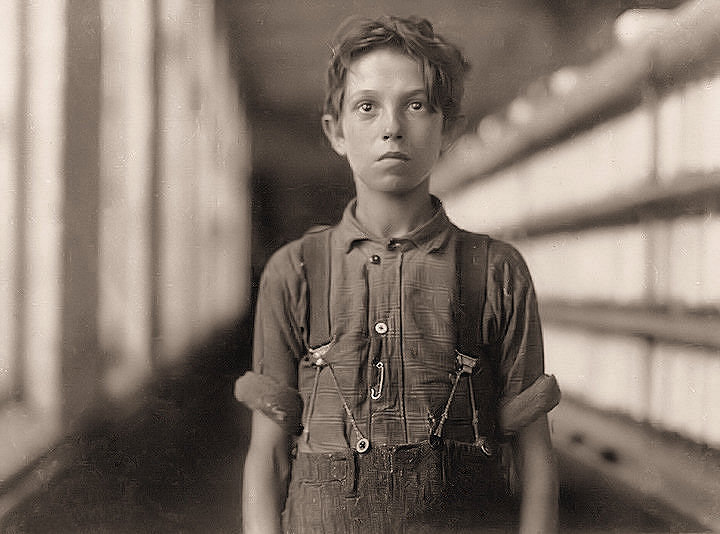
\includegraphics[width=3cm]{hine02}\par
\raggedright
\textit{Cover image: }
The cover image shows Jo Bodeon, a back-roper in the mule room at Chace Cotton Mill. Burlington, Vermont. This and other similar images in this book were taken by Lewis W. Hine, in the period between 1908-1912. These images as well as social campaigns by many including Hine, helped to formulate America's anti-child labour laws.
\end{minipage}\par
\vspace*{\baselineskip}
\begin{minipage}[b]{0.9\textwidth}
\raggedright
\setlength{\parskip}{0.5\baselineskip}
Copyright \copyright 2012  Dr Yiannis Lazarides\par
Permission is granted to copy, distribute and\slash or modify this document under the terms of the GNU Free Documentation License, version 1.2, with no invariant sections, no front-cover texts, and no back-cover texts.\par
A copy of the license is included in the appendix.\par
This document is distributed in the hope that it will be useful, but without any warranty; without even the implied warranty of merchantability or fitness for a particular purpose.
\end{minipage}
\vspace*{2\baselineskip}
\clearpage
}

%% Some special styles
\IfFileExists{changepage.sty}{\RequirePackage{changepage}}{}
\IfFileExists{rotating.sty}{\RequirePackage{rotating}}{}

%    \end{macrocode}
%
% \begin{macro}{\even@samplepage}

% \begin{macro}{\odd@samplepage}
%    \begin{macrocode}
\def\even@samplepage{%
 \begin{picture}(0,0)
   \put(\Xeven,\Yeven){\turnbox{90}{\Huge \textcolor{\watermark@textcolor}{\watermark@text}}}
\end{picture}
}
%% Define a macro to print SAMPLE PAGE IN THE MARGIN
\def\odd@samplepage{%
 \begin{picture}(0,0)
   \put(\Xodd,\Yodd){\turnbox{90}{\Huge \textcolor{\watermark@textcolor}{\watermark@text}}}
 \end{picture}
}
%    \end{macrocode}
% \begin{macro}{watermarktext}
%  Define the watermark words
%    \begin{macrocode}
\def\watermarktext#1{\gdef\watermark@text{\fontfamily{phv}\selectfont#1}}
\def\watermarktextcolor#1{\gdef\watermark@textcolor{#1}}
\watermarktext{SAMPLE PAGE}
\watermarktextcolor{purple}
%    \end{macrocode}
% \end{macro}
%    \begin{macrocode}
%% redefine LaTeX's plain as myplain for headings
\def\ps@samplepage{\let\@mkboth\@gobbletwo
 \let\@oddhead\odd@samplepage\def\@oddfoot{\reset@font\hfil\thepage}
 \let\@evenhead\even@samplepage\def\@evenfoot{\reset@font\thepage\hfil}}
%%
%
%% We define two macros to position the watermark on the page
\def\Xodd{500}
\def\Xeven{-70}\def\Yeven{-810}
\def\Yeven{-\expandafter\strip@pt\textheight}
\let\Yodd\Yeven


\cxset{blank page text/.store in=\blankpagetext@cx{#1}}

\def\cleardoublepage{\clearpage\if@twoside\ifodd\c@page\else
  \hbox{}
  \vspace*{\fill}
  \begin{center}
     \blankpagetext@cx      
  \end{center}
  \vspace{\fill}
  \thispagestyle{empty}
  \newpage
  \if@twocolumn\hbox{}\newpage\fi\fi\fi}

\parindent1.5em

%% Examples for documentation
\newcounter{texexp}[chapter]
\@addtoreset{c@texexp}{c@chapter}
\def\thetexexp{\thesection.\arabic{texexp}}
\tcbset{
texexp/.style={%
   fonttitle=\small\sffamily\bfseries, fontupper=\small, fontlower=\small},
  example/.code 2 args={\refstepcounter{texexp}\label{#2}}%
  \pgfkeysalso{texexp,title={Example \thetexexp\ #1}},
}


\newenvironment{texexp}[1]{\tcblisting{texexp,#1}}{\endtcblisting}
\newenvironment{example}[3][]{\tcblisting{example={#2}{#3},#1}}{\endtcblisting}
%%rename to avoid clashes with other classes that use it

\newenvironment{texexample}[3][]{\tcblisting{example={#2}{#3},#1}}{\endtcblisting}


% Define a macro name for the documentation
\def\athena{\textcolor{thered}{athena}}
% Be nice to hackers define a boolean to know if the package was loaded
\newif\if@athena
\@athenatrue
\begin{document}

\frontmatter
\pagestyle{empty}
\coverpage{hine02}{Yiannis Lazarides}{Published by Camel Press}

%\newgeometry{top=20mm,bottom=20mm,left=35mm,right=35mm}
\secondpage

\thispagestyle{samplepage}
%% temporary titles
% command to provide stretchy vertical space in proportion
\newcommand\nbvspace[1][1]{\vspace*{\stretch{#1}}}
% allow some slack to avoid under/overfull boxes
\newcommand\nbstretchyspace{\spaceskip0.5em plus 0.25em minus 0.25em}
% To improve spacing on titlepages
\newcommand{\nbtitlestretch}{\spaceskip0.6em}
\pagestyle{empty}
\begin{center}
\bfseries
\nbvspace[1]
\Huge
{\nbtitlestretch\huge
A NEW LOOK AT\\ LATEX BOOK DESIGN}

\nbvspace[1]
\normalsize

TO WHICH IS ADDED MANY USEFUL MACROS\\
AND THE \textbf{CHAPTERX} PACKAGE SO THAT\\
YOU CAN MAKE BEAUTIFUL BOOKS\\
%YOU CAN CODE LIKE A HAWK
\nbvspace[1]
\small BY\\
\Large DR YIANNIS LAZARIDES\\[0.5em]
%\footnotesize AUTHOR OF ``A WORKING ALGEBRA,'' ``WIRELESS TELEGRAPHY,\\
%ITS HISTORY, THEORY AND PRACTICE,'' ETC., ETC.

\nbvspace[2]

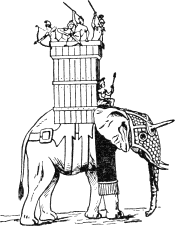
\includegraphics[width=1.5in]{pic37}
\nbvspace[3]
\normalsize

DOHA\\
\large
PUBLISHED IN THE WILD
\nbvspace[1]
\end{center}


\cxset{blank page text=\epigraph{We all agree that your theory is crazy. 
          But is it crazy enough?}{Niels Bohr}}

\mainmatter


\pagestyle{plain}
\tableofcontents

\setdefaults
% Set blank page epigraphs in main matter only

%\clearpage
%\end{document}

\cxset{toc image=true}
\@specialfalse
\chapter{Table of Contents Styling}

A number of experimental keys have been defined to handle the Table of Contents formatting. These will need to be revisited at the next version.


Firstly we define the width of the box that the page number is set. Use ems so that it does not need to be redefined for every change in font size.
Toc entries are treated as rectangular areas where the text
and probably a filler will be written. Let's draw such an
area (of course, the lines themselves are not printed):

\cxset{section font-weight=\bfseries}
\section{Width of page numbers and a very ong and really very long section numbering scheme}

The width of the page number is defined in pnumwidth

\section{test}

\section{Technical Details}

The macros of a table of contents are saved in an auxiliary file named \marg{jobname.toc} where you can find lines like this:

\subsection{The toc file}
\subsubsection{The structure of the toc file}
\begin{tcolorbox}[title=Extract from .toc file]
\begin{lstlisting}
\defcounter {refsection}{0}\relax 
\contentsline {chapter}{\numberline {1}Table of Contents Styling}{1}{chapter.1}
\defcounter {refsection}{0}\relax 
\contentsline {section}{\numberline {1.1}Width of page numbers and a very ong and really very long section numbering scheme}{1}{section.1.1}
\defcounter {refsection}{0}\relax 
\contentsline {section}{\numberline {1.2}test}{1}{section.1.2}
\defcounter {refsection}{0}\relax 
\contentsline {section}{\numberline {1.3}Technical Details}{1}{section.1.3}
\end{lstlisting}
\end{tcolorbox}

When the file is imported back the commands are expanded and the table of contents lines printed as shown below.


\section{The key value concept}



\begin{tcolorbox}[title=Extract from .toc file]
\defcounter {refsection}{0}\relax 
\contentsline {chapter}{\numberline {1}Table of Contents Styling}{1}{chapter.1}
\defcounter {refsection}{0}\relax 
\contentsline {section}{\numberline {1.1}Width of page numbers and a very ong and really very long section numbering scheme}{1}{section.1.1}
\defcounter {refsection}{0}\relax 
\contentsline {section}{\numberline {1.2}test}{1}{section.1.2}
\defcounter {refsection}{0}\relax 
\contentsline {section}{\numberline {1.3}Technical Details}{1}{section.1.3}
\end{tcolorbox}

The two important macros we need to get access to, in order to be able to have a flexible approach in formatting table of contents are \cs{contentsline} and \cs{numberline} and their dependencies.

The \cs{contentsline} definition triggers the calling of macros that start with \verb+l@+ and for the sectioning commands have typical formats such as \lstinline{l@chapter, l@section etc.}

\begin{tcolorbox}
\begin{lstlisting}
\def\contentsline#1{\csname l@#1\endcsname}  
\end{lstlisting}
\end{tcolorbox}

Ultimately if we wanted to seriously redefine the looks of a  toc chapter details we need to detail it in the l@chapter. This is defined in book.cls and has the form.

\begin{tcolorbox}
\begin{lstlisting}
\renewcommand*\l@chapter[2]{%
  %#1 number and title  #2 page number
  \ifnum \c@tocdepth >\m@ne
    \addpenalty{-\@highpenalty}%
    \vskip 1.0em \@plus\p@
    \setlength\@tempdima{1.5em}%
    \begingroup
      \parindent \z@ \rightskip \@pnumwidth
      \parfillskip -\@pnumwidth
      \leavevmode \bfseries \color{thegray}
      \advance\leftskip\@tempdima
      \hskip -\leftskip
      (#1)\nobreak\hfil \nobreak\hb@xt@\@pnumwidth{\hss#2\hspace*{3cm}}\par
      \penalty\@highpenalty
    \endgroup
  \fi}
\end{lstlisting}

\renewcommand*\l@chapter[2]{%
  %#1 number and title  #2 page number
  \ifnum \c@tocdepth >\m@ne
    \addpenalty{-\@highpenalty}%
    \vskip 1.0em \@plus\p@
    \setlength\@tempdima{1.5em}%
    \begingroup
      \parindent \z@ \rightskip \@pnumwidth
      \parfillskip -\@pnumwidth
      \leavevmode \bfseries \color{thegray}
      \advance\leftskip\@tempdima
      \hskip -\leftskip
      \colorbox{red}{\hbox to 10cm{\color{white}#1\hss #2}}\par
      \penalty\@highpenalty
    \endgroup
  \fi}
\l@chapter{1 test}{12}
\end{tcolorbox}


So far we have simplistically examined the formatting. Life can get a bit more complex if we want to have a layout as shown in Figure \ref{fig:toc}.

\begin{figure}[tp]
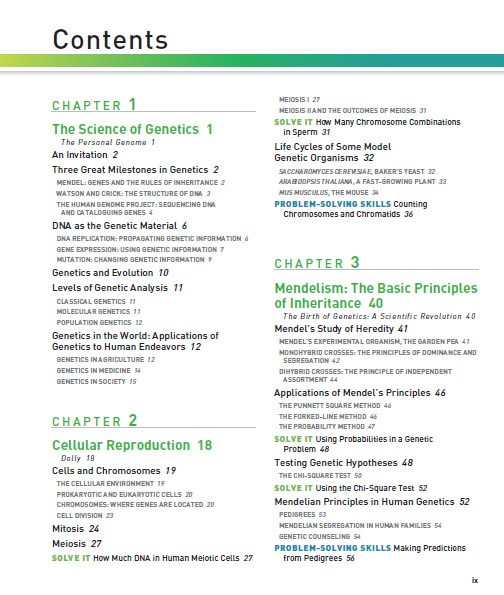
\includegraphics[width=0.8\textwidth]{contents01}
\caption{Complex table of contents layout.}
\label{fig:toc}
\end{figure}

\begin{tcolorbox}
\begin{lstlisting}
\renewcommand\l@chapter[3]{%
  %#1 number and title  #2 page number
  \ifnum \c@tocdepth >\m@ne
    \addpenalty{-\@highpenalty}%
    \vskip 1.0em \@plus\p@
    \setlength\@tempdima{1.5em}%
    \begingroup
      \parindent \z@ \rightskip \@pnumwidth
      \parfillskip -\@pnumwidth
      \leavevmode 
      \advance\leftskip\@tempdima
      \hskip -\leftskip
      \vbox{\raggedright#1\vskip1pt%
      \hrule width3cm height0.4pt}\par
      #2
      \penalty\@highpenalty
    \endgroup
  \fi}
\end{lstlisting}
% define three parameters the chapter number, title separate 
\renewcommand\l@chapter[3]{%
  %#1 number and title  #2 page number
  \ifnum \c@tocdepth >\m@ne
    \addpenalty{-\@highpenalty}%
    \vskip 1.0em \@plus\p@
    \setlength\@tempdima{1.5em}%
    \begingroup
      \parindent \z@ \rightskip \@pnumwidth
      \parfillskip -\@pnumwidth
      \leavevmode 
      \advance\leftskip\@tempdima
      \hskip -\leftskip
      \vbox{\raggedright#1\vskip1pt%
      \hrule width3cm height0.4pt}\par
      #2
      \penalty\@highpenalty
    \endgroup
  \fi}
\cxset{chapter color=thegreen}
\l@chapter{\color{\chaptercolor@cx}\bfseries\chaptername\hskip1em\thechapter}{A Chapter Title}{12}
\end{tcolorbox}


In this figure only the chapter number is shown, no page number and the section details are layed down in a two column format.


If we take a similarly flexible approach of redefining l@chapter we can try and format the toc shown in Figure \ref{fig:tocsteward}.

\begin{figure}[tp]
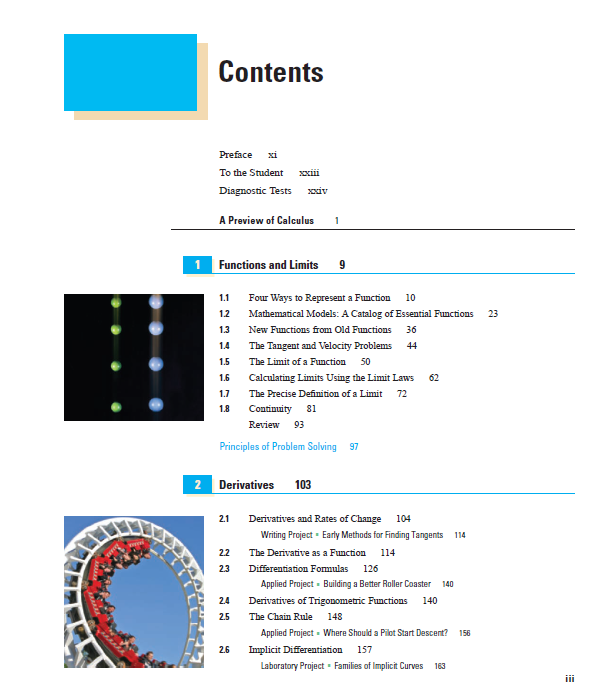
\includegraphics[width=0.8\textwidth]{contents02}
\caption{Complex table of contents layout.}
\label{fig:tocsteward}
\end{figure}

\begin{tcolorbox}
\begin{lstlisting}
\renewcommand\l@chapter[3]{%
  %#1 number and title  #2 page number
  \ifnum \c@tocdepth >\m@ne
    \addpenalty{-\@highpenalty}%
    \vskip 1.0em \@plus\p@
    \begingroup
      \parindent \z@ 
      \leavevmode 
      \vbox{\raggedright\colorbox{blue}{\color{white}\bfseries\sffamily#1} #2\qquad  #3\vskip0pt%
      \color{blue}\hrule width0.7\textwidth height0.4pt}\par
      \penalty\@highpenalty
    \endgroup
  \fi}
\end{lstlisting}
% define three parameters the chapter number, title separate
\cxset{
  toc chapter name/.store in=\chaptername,
  toc chapter name color/.code=\gdef\tocchapternamecolor@cx{#1},
  toc title color/.store in=\toctitlecolor@cx,
  toc title font-weight/.store in=\toctitlefontweight@cx,
  toc title before/.store in=\toctitlebefore@cx,
  toc title after/.store in=\toctitleafter@cx,
  toc after pagenumber/.store in=\tocafterpagenumber@cx,
}  
\cxset{toc title color=theblue,  %interfers with links
       toc title font-weight=\fontfamily{ptm}\selectfont\bfseries ,
       toc title before=\hspace*{0.5em},
       toc title after=\hspace*{1.5em},
       toc after pagenumber=,
}
\renewcommand\l@chapter[3]{%
  %#1 number and title  #2 page number
  \ifnum \c@tocdepth >\m@ne
    \addpenalty{-\@highpenalty}%
    \vskip 1.0em \@plus\p@
    \begingroup
      \parindent \z@ 
      \leavevmode 
      \vbox{\raggedright\colorbox{blue}{\color{white}%
             \sffamily#1 }%
%% title formatting 
        {\toctitlebefore@cx\color\toctitlecolor@cx\toctitlefontweight@cx% 
          #2%
          \toctitleafter@cx}% font info
          #3\tocafterpagenumber@cx\vskip0pt%
              \color{blue}
              \hrule width0.7\textwidth height0.4pt}\par
      \penalty\@highpenalty
    \endgroup
  \fi}

\cxset{chapter color=thegreen}
\l@chapter{12}{A Chapter Title}{\thepage}%where is page number coming?

\l@chapter{12}{A Chapter Title}{\thepage}
\end{tcolorbox}


The above method of redefinition is a bit more flexible and can be extended to cover all cases that do not fall broadly with the standard class provisions.



The \cs{addcontentsline}{\marg{table}\marg{type}\marg{entry} command allows the user to add an entry to a table of contents. The command adds the entry
\cs{contentsline}\marg{type}\marg{entry}\marg{page} to the \marg{.table} file.



For example the chapter,

\begin{lstlisting}
 \addcontentsline{toc}{chapter}%
       {\protect\numberline{\thechapter}#1}

\def\addcontentsline#1#2#3{%
  \addtocontents{#1}{\protect\contentsline{#2}{#3}{\thepage}}}

\def\contentsline#1{\csname l@#1\endcsname}  
\end{lstlisting}

The contents line is the line that hold the specific commands for a section formatting such as l@chapter

addcontentsline(3)

addtocontents(3) save to file protected


\chapter{Fonts}

\fontspec[Numbers={Proportional,OldStyle}]
{TeX Gyre Adventor}
`In 1842, 999 people sailed 97 miles in
13 boats. In 1923, 111 people sailed 54
miles in 56 boats.' \bigskip




\fontspec[
UprightFeatures={Color = 220022,
SmallCapsFeatures = {Color=115511}},
ItalicFeatures={Color = 2244FF,
SmallCapsFeatures = {Color=112299}},
BoldFeatures={Color = FF4422,
SmallCapsFeatures = {Color=992211}},
BoldItalicFeatures={Color = 888844,
SmallCapsFeatures = {Color=444422}},
]{TeX Gyre Termes}
Upright {\scshape Small Caps}\\
\itshape Italic {\scshape Italic Small Caps}\\
\upshape\bfseries Bold {\scshape Bold Small Caps}\\
\itshape Bold Italic {\scshape Bold Italic Small Caps}


\end{document}

\chapter{Introduction}



Browse any books in a library or bookshop and the striking thing is that their design is very individualistic. They might have similarities but their main features vary. In many respects they resemble people's faces where minor differences have striking effects.

This package arose out of a question at stackexchange. How to redefine chapter heads. Having seen the popularity of pgf I realized that LaTeX users prefer this method of styling rather the traditional LaTeX method. 

The user interface can be extended to basically all major packages. The principle is to keep to a minimum changes that can affect the LaTeX core commands. If there are any additions a key setting is provided to be able to revert back to normal LaTeX.

The workflow can be simplified. In addition I want to believe that the interface can provide a useful addition to the open source community and that other people will contribute libraries, which will be simpler to write.

\section{Why this package}

Most people when they get started with \LaTeX\ will either use one of the standard classes such as the \file{book.cls} or one of the generic classes notably koma-script or memoir. Most students will be forced to use on of the many thesis classes available. 

\section{The key value concept}

The key-value concept that originated with \LaTeX\ has been extended many times, the last and most serious implementation of it by Tantau in the PGF package. What essentially Tantau allows us to do is to use a scripting language to script TeX code. The TikZ and pgfplots packages are two major packaged that use keys effectively. Their popularity is gowing and what \athena\ does is to offer a user interface that in many respects.



\section{Improvements in the user interface}

\section{On typography}

This package hopefully will assist in improving the typography of books set with \LaTeX\ and this package. Any typographical comments on the various styles are my own and not necessarily correct. Like fashion and art typography has opinions rather than absolute truths. In many styles the design is slightly adapted to blend a bit better with this manual. Also I did not select fonts as per the samples but this is left on you the user to decide.

I selected samples based on their programming demands and not on  typography. For example Chapter\ref{style:46}, was selected to demonstrate the use of TikZ to produce leaders and decorations and not on its looks, which is not terribly attractive.
%
%\pagestyle{myheadings}
%\markboth{test}{test}
%\lipsum\lipsum\lipsum
%% CHAPTER OPENINGS

\cxset{custom/.code=\gdef\customdesign@cx{\csname#1\endcsname}\@specialtrue,
       fill/.store in=\fill@cx}
%\cxset{stefan/.style={fill=purple, title font-color=\color{white},
%          custom=tikzspecials}}


\cxset{steward/.style={
  offsety/.store in=\soffsety,
  image/.store in=\image@cx,
  texti/.store in=\texti@cx,
  textii/.store in=\textii@cx,
}}

%\cxset{steward/.style={
%   custom=tikzspecial,
%  offsety/.store in=\soffsety,
%  image/.store in=\image@cx,
%  texti/.store in=\texti@cx,
%  textii/.store in=\textii@cx,
%}}

\newcommand\tikzspecial[2][]{%
\fancypagestyle{plain}{%
\lhead{}\rhead{}
\chead{}
\cfoot{}
\lfoot{}
\rfoot{\thepage}
\def\footrule#1{{\color{blue}%
  \hrule width\paperwidth}\vskip3pt
}

\renewcommand{\headrulewidth}{0pt}
\renewcommand{\footrulewidth}{0.4pt}}

\clearpage

\begin{tikzpicture}[remember picture,overlay]
% Main shading block
\node [xshift=5cm,yshift=-\paperheight] at (current page.north west)
[text width=0.98\textwidth,text height=\paperheight, fill=thecream!30,rounded corners,above right]
{};
\node [xshift=6.5cm,yshift=-1.5cm-\soffsety] at (current page.north west)
[text width=0.9\textwidth,below right]{\sffamily \bfseries \huge #2};

\node [xshift=3cm,yshift=-1.5cm] at (current page.north west)
[text width=3cm,align=center,minimum height=2.5cm, fill=blue,below right]
{$$\text{\HHUGE\bfseries\sffamily\color{white}\thechapter}$$
\par\vspace*{3pt}
};

\node [xshift=-0.2cm,yshift=-21.5cm] at (current page.north west)
[text width=3cm,above right]%
{\includegraphics[width=1.0\paperwidth]{./chapters/\image@cx}};
% second box left
\node [xshift=3cm,yshift=-19.5cm] at (current page.north west)
[text width=9cm,minimum height=2.5cm,inner sep=0.5em, fill=blue,below right]
{\color{white}
  \bfseries\sffamily \texti@cx
};
% Last block
\node [xshift=6.5cm,yshift=-26cm] at (current page.north west)
[text width=12cm,above right]
{\textii@cx
};
\end{tikzpicture}
\par
\clearpage
}

%%%%%%%%%%%%%%%%%%%%%%%%%%%%%%%%%%%%%%%%%%%%%%%

%% CHAPTER OPENINGS
\cxset{steward/.style={
  offsety/.store in=\soffsety,
  image/.store in=\image@cx,
  texti/.store in=\texti@cx,
  textii/.store in=\textii@cx,
}}


\renewcommand\tikzspecial[2][]{%
\fancypagestyle{plain}{%
\lhead{}\rhead{}
\chead{}
\cfoot{}
\lfoot{}
\rfoot{\thepage}
\renewcommand{\footrule}{{\color{blue}%
  \hrule width\paperwidth}\vskip3pt
}
\renewcommand{\headrulewidth}{0pt}
\renewcommand{\footrulewidth}{0.4pt}}


\begin{tikzpicture}[remember picture,overlay]
% Main shading block
\node [xshift=5cm,yshift=-\paperheight] at (current page.north west)
[text width=0.98\textwidth,text height=\paperheight, fill=thecream!30,rounded corners,above right]
{};
\node [xshift=6.5cm,yshift=-1.5cm-\soffsety] at (current page.north west)
[text width=0.9\textwidth,below right]{\sffamily \bfseries \huge #2};

\node [xshift=3cm,yshift=-1.5cm] at (current page.north west)
[text width=3cm,align=center,minimum height=2.5cm, fill=blue,below right]
{$$\text{\HHUGE\bfseries\sffamily\color{white}\thechapter}$$
\par\vspace*{3pt}
};

\node [xshift=-0.2cm,yshift=-21.5cm] at (current page.north west)
[text width=3cm,above right]%
{\includegraphics[width=1.0\paperwidth]{./chapters/\image@cx}};
% second box left
\node [xshift=3cm,yshift=-19.5cm] at (current page.north west)
[text width=9cm,minimum height=2.5cm,inner sep=0.5em, fill=blue,below right]
{\color{white}
  \bfseries\sffamily \texti@cx
};
% Last block
\node [xshift=6.5cm,yshift=-26cm] at (current page.north west)
[text width=12cm,above right]
{\textii@cx
};
\end{tikzpicture}

\par
\clearpage
}

\@specialtrue
\cxset{steward,
  numbering=arabic,
  custom=tikzspecial,
  offsety=0cm,
  image=hine02,
  texti={When Lamport designed the original \LaTeX\ sectioning commands, limitations of computer power forced him to restrict the abstraction of complicated chapter layouts. With current tools available improvements are much easier to program.},
%
  textii={In this chapter we discuss a method that allows the production of fancy chapter headings and formatting, based on a set of key values. Central  to this process is the separation of content from presentation.
We also discuss the basic formatting tools that are available and how one can modify them to mould new book designs.
 }
}

\clearpage




%\@specialtrue
%\cxset{steward,
%  numbering=arabic,
%  custom=tikzspecial,
%  offsety=0cm,
%  image=hine02,
%  texti={When Lamport designed the original \LaTeX\ sectioning commands, limitations of computer power forced him to restrict the abstraction of complicated chapter layouts. With current tools available improvements are much easier to program.},
%%  textii={In this chapter we discuss a method that allows the production of fancy chapter headings and formatting, based on a set of key values. Central  to this process is the separation of content from presentation.
%%We also discuss the basic formatting tools that are available and how one can modify them to mould new book designs.
% %}
%}

\clearpage

\chapter{Designing Chapters}

\section{Introduction}

For too long, the act of printing something in and of itself has been placed on too high a pedestal. The true value of an object lies in what it says, not its mere existence. And in the case of a book, that value is intrinsically connected to content. The aim of this package is to try and provide a bridge between separating content from presentation.

A new chapter must make a good impression and must give an immediate signal that something different is going to be written. Traditionally chapter openings in LaTeX are an unimpressive and dry event. Our aim is to brighten it up a bit, while keeping true separation of content from presentation.

\section{Package Usage}

To use the package include it just like any other package:

\begin{tcolorbox}
\begin{lstlisting}
\documentclass{book}
\usepackage{chaptersx}
\cxset{style13}
\begin{document}
\chapter{Introduction}
\end{document}
\end{lstlisting}
\end{tcolorbox}

The command \cs{cxset} sets the default style for the example to the style defined as \marg{style13}. The package currently offers over 50 styles and numerous keys to manipulate them further.

\section{Chapter opening page}

The standard LaTeX classes offer only two options to either open a chapter on an odd page or at any page. This package offers five alternatives:

\keyval{chapter opening}{\marg{any, left, right, anywhere, ifafter}}{The various keys enable any combination to be used.}

\begin{marglist}
\item [any] Opens a chapter at any page, either verso or recto.
\item [left] Opens a chapter on an even page
\item [right] Opens a chapter on a right page.
\item [anywhere] Opens a chapter at the point where the \cs{chapter} is typed.
\item [none] Alias for \marg{anywhere}.
\item [ifafter] Opens a chapter at the next page if the page has material that does not exceed a certain portion of \cs{textheight}.
\end{marglist}

To change a setting you just modify the value of the key \option{chapter opening} to one of the values described earlier.

\begin{tcolorbox}
\begin{lstlisting}
\cxset{chapter opening=anywhere}
\end{lstlisting}
\end{tcolorbox}

\@specialfalse
\cxset{chapter toc=false}
\begin{tcblisting}{title=Inline Chapter Example}
\cxset{chapter opening=anywhere, chapter before=\bigskip, chapter font-family=\sffamily,title font-family=\sffamily}

\lipsum[2]
\chapter{Inline Chapter Example}
\lipsum[3]
\chapter{Another Inline Chapter Example}
\lipsum[4]
\end{tcblisting}

Examples for other types of chapter openings follow in the rest of the documentation.
\subsection{Blank pages before chapters}
In the standard LaTeX book class when the openany option is not given or in the report class when the openright is given, chapters start at odd-numbered pages. This can cause a blank page to be printed. Some book designers prefer this page to be completely empty, without any headers or footers. This cannot be done with \lstinline{\thispagestyle} as this command will have to be issued on the \textit{previous} page. However by a suitable redefinition of the 
\lstinline{\clearpage} this can be done automatically.
\medskip

\begin{tcolorbox}
\begin{lstlisting}
\makeatletter
\def\cleardoublepage{\clearpage\if@twoside\ifodd\c@page\else
  \hbox{}
  \vspace*{\fill}
  \begin{center}
    This page left intentionally blank.
  \end{center}
  \vspace{\fill}
  \thispagestyle{empty}
  \newpage
  \if@twocolumn\hbox{}\newpage\fi\fi\fi}
\makeatother 
\end{lstlisting}
\end{tcolorbox}
\medskip

This is achieved easily by setting the following options:
\bigskip

\begin{tcolorbox}
\lstinline{chapter blank page=empty}\par
\lstinline{chapter blank page text=Some text.}\par
\lstinline{chapter blank page=plain}\par
\end{tcolorbox}
\medskip

The last one refers to a \lstinline!\thispagestyle{plain}!.

\section{Keys for chapter head formatting}

A chapter heading can be considered of being constructed of several parts, the \textit{chapter number}, the chapter name typically \textit{chapter} and the \textit{title}. Predefined keys handle all the elements of formatting. Additional keys are defined to handle other elements such as inclusion of images or producing complicated examples with graphics constructed with TikZ or other similar packages.

\medskip

\keyval{chapter numbering font-size}{\oarg{sizing commands}}{}.
\keyval{chapter numbering font-family}{\oarg{sizing commands}}{}.

\subsection{Keys for numbering}
Chapter numbering follows that of the standard \LaTeX\ classes and is extended to cover some additional cases such as fully spelled out numbers.

\keyval{number numbering}{\oarg{alph,Alph,roman,Roman,none,WORDS,words}}{Style of numbering.}
\medskip

\parindent1.5em

Note that the package uses Heiko Oberdiek's package alphalph to allow for alphabetic numbering that extends beyond the normal 26 letters of the alphabet.

\medskip

\begin{marglist}
\item [arabic] Despite that the Arabs call what the West calls Arabic numbers Indian numbers, we provide the value arabic to have normal numbers printed.
\item [alph] Lowercase alphabetic numbering.
\item [Alph] Uppercase alphabetic numbering.
\item [roman] Lowercase roman numbering.
\item [Roman] Uppercase roman numbering.
\item [words] 
\item [WORDS]
\item [Words] Prints the number in words and capitalizes the first letter, for example the number 21 will be printed as `Twenty One'\footnote{Currently limited to the first hundred numbers}.
\item [none] This is equivalent to using the star version of the command. It does not print any number and does not increment the chapter counter.\footnote{I am ambivalent about this, perhaps it will be better to increment it, as it can give a more general approach.}
\end{marglist}

\cxset{chapter opening=anywhere, numbering=Roman}

\begin{tcblisting}{}
\cxset{numbering=Roman}
\chapter{Roman numbering}
\end{tcblisting}

\clearpage

\begin{tcblisting}{title=Chapter number in words}
\cxset{numbering=WORDS}
\chapter{Literal numbering}
\end{tcblisting}

\cxset{numbering=arabic}


\subsection{Setting font information}
\subsection{Letter spacing}  

Chapter letter spacing can be achieved using the soul package in a combination with the key spaceout.
\medskip



\keyval{chapter spaceout}{\marg{soul}}{Uses the soul package to space out the lettering of chapter, number or the chapter name.}\par\medskip

\parindent1.5em

The following examples illustrate the usage.

\begin{tcblisting}{}
\cxset{numbering=Roman,
         chapter spaceout=none,
         title spaceout=soul,
         title font-size=\Large,
         title font-family=\rmfamily, 
         title font-shape=\scshape}
\chapter{Letter Spacing}
\end{tcblisting}

\begin{tcblisting}{}
\cxset{chapter spaceout=soul,numbering=arabic, title spaceout=soul}
\chapter{Chapter title}
\end{tcblisting}


\subsection{Styling the title}

Similarly to the number and chapter styling keys exist for styling the title. We summarize the available standard keys below:
\medskip

  \keyval{chapter title font-family}{\marg{family}}{Selects a predefined font family}
  \keyval{chapter title font-weight}{\marg{\cs{bfseries},\cs{normalseries}}}{Font weight.}
  \keyval{chapter title font-size}{\marg{\cs{large},\cs{Large},\cs{huge},\cs{Huge},\cs{HUGE},\cs{HHuge}}}{Font sizing command.}
  \keyval{chapter title font-color}{}{}
  \keyval{chapter title spaceout}{\marg{soul,none}}{}
%  \keyval{title spaceout}/soul/.code={\@titlespaceouttrue},
%  title spaceout/none/.code={\@titlespaceoutfalse},
%  title font/.style={title font-family=#1},
  \keyval{title before}{}{}
 \keyval{title after}{}{}
  \keyval{title beforeskip}{}{}
  \keyval{title afterskip}{}{}


\begin{tcblisting}{}
\cxset{style13, chapter spaceout=none}
\chapter{Chapter Title Styling}
\end{tcblisting}

The last example illustrated the use of a predefined style \oarg{style13} and overriding some of the parameters.


\cxset{chapter opening=right}
\section{Table of Contents}\index{table of contents!key settings}

Traditionally a chapter will be added to the Table of Contents if the \cs{chapter} command is issued. The starred version will not produce a number and will not add a contents line. Since we have adopted an approach where we use a key value interface we can dispense with the starred version of the command, by setting the \option{chapter toc} option to false. For example if we want to define a command for a ``Foreward'' or ``Epiloque'' without wishing them to be added to the table of contents we can use the following setting.\index{Foreward!definitions}\index{Epilogue!definitions}

\begin{tcblisting}{}
\cxset{chapter toc=false, name=, numbering=none,}
\chapter{Foreward}
\lorem
\end{tcblisting}

Please note that when numbering=none the chapter number is not available anymore and yo may have to reset it if required again. Although this might be seen as rather cumbersome than simply using \cs{chapter*} the advantage is consistency in the user interface and the use of appropriate semantic definitions for all sectioning commands thus achieving a bit more separation of context from style.


\cxset{chapter toc=true}

\section{Defining styles}

Named styles can be defined using the standard \textsc{PGF} conventions. To define a style for the forward above we can use:

\begin{tcblisting}{}
\cxset{foreward/.style={chapter toc=false, 
          name=,
          title font-size=\Large,
          title font-family=\sffamily,
          numbering=none}}
\cxset{foreward}
\chapter{Foreward}
\lorem
\end{tcblisting}

\cxset{numbering=arabic}
\section{Creating semantic names for commands and environments}

To keep our search for semantic commands and true separation of contents it is prudent to define some macros for typesetting the  `foreward' section.

\begin{tcblisting}{}
\cxset{foreward/.style={chapter toc=false, 
          name=,
          title font-size=\Large,
          title font-family=\sffamily,
          numbering=none}}
\newcommand\forewardname{foreward}
\expandafter\newenvironment\expandafter{\forewardname}{%
\cxset{foreward}\chapter{Foreward}}%
{}

\begin{foreward}
\lorem
\end{foreward}

\end{tcblisting}

Notice the use of a new command \cs{forewardname} to allow for internationlization using Babel or other methods. One is tempted to let the English name, but a better approach perhaps is to define both.





\cxset{chapter toc=true,numbering=arabic,name=Chapter}
\cxset{blank page text=\epigraph{The great tragedy of science is the slaying of a beautiful theory
by an ugly fact.}{Thomas Huxley}}

\chapter{Epigraphs}\index{epigraphs}
\epigraph{Example is the school of mankind, and they
will learn at no other.}{Letters on a Regicide Peace}



\section{Introduction}
Epigraphs or quotations before or after chapters are quite common in books. Peter Wilson's epigraph package, does a good job and we have adapted it where necessary to allow for a key value interface. The command:

\cs{epigraph}\marg{text}\marg{source}. By default the epigraph is placed at the right
hand side of the textblock, and the \marg{source} is typeset at the bottom right of the \marg{text}. Numerous settings allow for manipulating the width of the epigraph, the location and other variables. If the package is available we use it otherwise we use other internal commands.



\section{Key-value interface}
The key value interface provided by the package is shown below. It mostly follows the naming conventions of the epigraph package to make the transition easier for experienced users.
\medskip

\keyval{epigraph align}{\marg{left, center, right}}{A font-size command such as \cs{footnotesize}, \cs{small} and other similar commands.}

\keyval{epigraph rule width}{\marg{dim}}{A font-size command such as \cs{footnotesize}, \cs{small} and other similar commands.}

\keyval{epigraph font-size}{\marg{dim}}{A font-size command such as \cs{footnotesize}, \cs{small} and other similar commands.}

\keyval{epigraph beforeskip}{\marg{dim}}{Space before the epigraph.}
\keyval{epigraph afterskip}{\marg{dim}}{Space after the epigraph.}
\keyval{epigraph source align}{\marg{left, center, right}}{Align the source text to the right, left or center.}
\keyval{epigraph source font-size}{\marg{dim}}{Align the source text to the right, left or center.}
\keyval{epigraph source font-shape}{\marg{dim}}{Align the source text to the right, left or center.}
\keyval{epigraph source font-family}{\marg{dim}}{Align the source text to the right, left or center.}
\keyval{epigraph source font-weight}{\marg{bold,normal}}{Align the source text to the right, left or center.}


\section{Example usage}
To set the style and an example usage is shown in .

\begin{example}{epigraph example}{}
\cxset{epigraph width=0.5\linewidth,
       epigraph font-size=\small,
       epigraph rule width=0.4pt,
       epigraph align=right,
       epigraph source align=right,
       epigraph text align=right}

%\chapter{Epigraphs}\index{epigraphs}
\epigraph{Example is the school of mankind, and they
will learn at no other.}{Letters on a Regicide Peace}
\end{example}

Another example for a somewhat longer quote:

\begin{example}{epigraph example}{}
\cxset{epigraph width=0.5\linewidth,
          epigraph font-size=\small,
          epigraph rule width=0.4pt,
          epigraph align=left,
          epigraph source align=right,
          epigraph text align=left}
%\chapter{Epigraphs}\index{epigraphs}
\epigraph{Everything written with vitality expresses that vitality; there are no dull subjects, only dull minds.}{Raymond Chandler\\\textit{Letters on a Regicide Peace}}
\end{example}

More usage examples can be found in relevant style examples (See Chapter~\ref{ch:41}) for a rather nice example with non-traditional alignment.

\section{Epigraphs on empty pages}

When a chapter open on an odd page sometimes the  previous page is left empty. Some book designers add the words ``this page left intentionally blank'' and other might add a quote. To add such a quote use:

\begin{tcolorbox}
\begin{lstlisting}
\cxset{blank page text=\epigraph{The great tragedy of science is the slaying of a beautiful theory
by an ugly fact.}{Thomas Huxley}}
\end{lstlisting}
\end{tcolorbox}


%%%%%%%%%%%%%%%%%%%%%%%%%%%%%%%%%%%%%%%%%%%%%%%%%
%  SECTIONING COMMANDS
\@specialtrue
\cxset{steward,
  numbering=arabic,
  custom=tikzspecial,
  offsety=0cm,
  image=hine03,
  texti={When Lamport designed the original \LaTeX\ sectioning commands, limitations of computer power forced him to restrict the abstraction of complicated chapter layouts. With current tools available improvements are much easier to program.},
%
  textii={In this chapter we discuss a method that allows the production of fancy chapter headings and formatting, based on a set of key values. Central  to this process is the separation of content from presentation.
We also discuss the basic formatting tools that are available and how one can modify them to mould new book designs.
 }
}



\raggedbottom

\chapter{Lower Level Headings}
\@specialfalse

\section{Introduction}

Good book design dictates that sectioning styles follow that of the general book design and theme. An academic publication for example might have chapters and section numbered in arabic numerals, whereas a high school textbook might have sections marked in colored boxes.

Similarly to the chapter key value interface, the package offers a key value interface to adjust sectioning command parameters. 



\cxset{section beforeskip={10pt},
      section indent=0pt}
\cxset{section afterskip={10pt}}
\renewsection

\section{Section styling}

In a similar fashion to the chapter commands the following keys are provided.

\subsection{Fonts and numerals}

Font and numeral keys are shown below.
\medskip

  \keyval{section font-size}{\marg{cmd}}{Font size command such as \cs{large.}}
  \keyval{section font-weight}{\marg{cmd}}{Font weight command such as \cs{bfseries.}}
  \keyval{section font-family}{\marg{cmd}}{Font family command such as \cs{sffamily.}}
  \keyval{section font-shape}{\marg{cmd}}{Font shape command such as \cs{itshape}}
  \keyval{section color}{\marg{color}}{Color of section.}
  \keyval{section numbering}{\marg{arabic|roman|Roman|alph|Alph|words|WORDS}}{Section number style.}
  \begin{marglist}
  \item [arabic] Typesers the section number in arabic numerals.
  \item [roman] Typesets the section number in lowercase roman numerals.
  \item [Roman] Typesets the section number in uppercase roman numerals.
  \item [alph] Typesets the section number in lowercase alphabetic numbering.
  \item [Alph] Typesets the section number in uppercase alphabetic numerals.
  \item [words] Typesets the numbers in words (lowercase).
  \item [WORDS] Typesets the number in words (uppercase). 
  \end{marglist}

\subsection{Skip and indentation commands} 

The keys for indentaion and above and below skips are shown below.
\medskip

\keyval{section beforeskip}{}{}
\keyval{section afterskip}{}{}
\keyval{section indent}{\marg{dim}}{Indentation from margin as per standard LaTeX class definitions.}
\keyval{section spaceout}{}{}
\begin{marglist}
 \item[soul]
 \item[none]
\end{marglist}

\subsection{align}

\keyval{section align}{\marg{cmd}}{One of the alignment commands centering, ragged right, raggedleft}

\subsection{Hooks}

Hooks for adding material are shown in the following sketch.
\medskip

\fbox{aboveskip}

\fbox{indent} \fbox{number}\fbox{hook}\fbox{title}

\fbox{belowskip}

%\lipsum

\section{Example usage}

\cxset{
 chapter toc=false,
 name=CHAPTER,
 numbering=arabic,
 number font-size=\huge,
 number font-family=\sffamily,
 number font-weight=\bfseries,
 number before=,
 number dot=,
 number after=\hspace{1em},
 number position=rightname,
 chapter opening=anywhere,
 chapter font-family=\sffamily,
 chapter font-weight=\bfseries,
 chapter font-size=\huge,
 chapter before={\vspace*{0.1\textheight}\hfill},
 chapter after={\hfill\hfill\vskip0pt\thinrule\par},
 chapter color={black!90},
 number color=\color{black!90},
 title beforeskip={\vspace*{30pt}},
 title afterskip={\vspace*{30pt}\par},
 title before={\hfill},
 title after={\hfill\hfill},
 title font-family=\sffamily,
 title font-color=\color{black!90},
 title font-weight=\bfseries,
 title font-size=\huge,
%%%%%%%%%% Sections
 section font-size=\LARGE,
 section font-weight=\normalfont,
 section font-family=\sffamily,
 section align=\centering,
 section numbering=arabic,
 section indent=0em,
 section align=\centering,
 section beforeskip=20pt,
 section afterskip=10pt,
 section spaceout=soul,
 section font-shape=\itshape,
}
\cxset{book/.style={
 section numbering=arabic,
 section font-size=\Large,
 section font-weight=\bfseries,
 section font-family=\rmfamily,
 section font-shape=\normalfont,
 section align=\raggedright,
 %section numbering custom=\color{gray}{Section} (\thechapter-\@arabic\c@section),
 subsection font-size=\large
 section indent=0em,
 section beforeskip=-3.5ex \@plus -1ex\@minus -0.2ex,
 section afterskip=2.3ex\@plus.2ex,
 subsection beforeskip=-3.5ex \@plus -1ex\@minus -0.2ex,
 subsection afterskip= 1.5ex \@plus .2ex,
}}


\begin{example}{Adjusting section parameters}{}
\cxset{ section font-size=\LARGE,
 section font-weight=\normalfont,
 section font-family=\sffamily,
 section align=\centering,
 section numbering=(roman),
 section indent=0em,
 section align=\centering,
 section beforeskip=20pt,
 section afterskip=10pt,}
\chapter{A First Look at the Sectioning Keys}
\section{First section}
\lorem
\end{example}

One notable thing to keep in mind is that the numbering of the chapter is independent of that for the section, so if you need to have strange combinations rather define a section numbering custom.\index{section formatting!vertical space}

\cxset{section numbering=arabic}
\subsection{Adjusting vertical spaces}

Perhaps the most important issues we need to consider is the adjusting of vertical spaces; example~\ref{ex:latex}, that follows illustrates settings from the Octavo class and compare them with those of standard the \LaTeXe\ book class. The Octavo class through settings that are based on baselineskip fractions and multiples endeavours to achieve a grid layout. The class also tones down the `loudness' of some of the headings compared to those of the book class.


\cxset{octavo/.style={
 section font-size=\large,
 section font-weight=\normalfont,
 section font-family=\rmfamily,
 section font-shape=\scshape,
 section indent=0em,
 section align=\centering,
 section beforeskip=-1.666\baselineskip\@minus -2\p@,
 section afterskip=0.835\baselineskip \@minus 2\p@,
 subsection numbering=none,
 subsection font-family=\rmfamily,
 subsection font-size=\normalfont,
 subsection font-shape=\scshape,
 subsection font-weight=\normalfont,
 subsection indent=1em,
 subsection align=\raggedright,
 subsection beforeskip=-0.666\baselineskip\@minus -2\p@,
 subsection afterskip=0.333\baselineskip \@minus 2\p@
 }}




\cxset{book/.style={
 section numbering=arabic,
 section font-size=\Large,
 section font-weight=\bfseries,
 section font-family=\rmfamily,
 section font-shape=\normalfont,
 section align=\raggedright,
 %section numbering custom=\color{gray}{Section} (\thechapter-\@arabic\c@section),
 subsection font-size=\large,
 section indent=0em,
 section beforeskip=-3.5ex \@plus -1ex\@minus -0.2ex,
 section afterskip=2.3ex\@plus.2ex,
 subsection font-size=\large,
 subsection font-weight=\bfseries,
 subsection numbering=arabic,
 subsection indent=0pt,
 subsection beforeskip=-3.5ex \@plus -1ex\@minus -0.2ex,
 subsection afterskip= 1.5ex \@plus .2ex,
}}

\cxset{octavo headings/.style={%
 section numbering=none,section font-size=\large,section font-weight=\normalfont,
 section font-family=\rmfamily, section font-shape=\scshape,
 section indent=0em, section align=\centering, section beforeskip=-1.666\baselineskip\@minus -2\p@,
 section afterskip=0.835\baselineskip \@minus 2\p@, subsection numbering=none,
 subsection font-family=\rmfamily, subsection font-size=\normalfont, subsection font-shape=\scshape,
 subsection font-weight=\normalfont, subsection indent=1em, subsection align=\raggedright,
 subsection beforeskip=-0.666\baselineskip\@minus -2\p@,
 subsection afterskip=0.333\baselineskip \@minus 2\p@,
 subsubsection numbering=none,
 subsubsection font-family=\rmfamily,
 subsubsection font-size=\normalfont,
 subsubsection font-shape=\itshape,
 subsubsection font-weight=\normalfont,
 subsubsection indent=1em,
 subsubsection align=\raggedright,
 subsubsection beforeskip=-0.666\baselineskip\@minus -2\p@,
 subsubsection afterskip=0.333\baselineskip \@minus 2\p@,
 paragraph numbering=none,
 paragraph font-family=\rmfamily,
 paragraph font-size=\normalfont,
 paragraph font-shape=\normalfont,
 paragraph font-weight=\normalfont,
 paragraph indent=-1em,
 paragraph align=\raggedright,
 paragraph beforeskip=\z@,
 paragraph afterskip=0\p@,
% subparagraph numbering=none,
% subparagraph font-family=\rmfamily,
% subparagraph font-size=\normalfont,
% subparagraph font-shape=\normalfont,
% subparagraph font-weight=\normalfont,
% subparagraph indent=0em,
% subparagraph align=\raggedright,
% subparagraph beforeskip=\z@,
% subparagraph afterskip=0\p@,
}}
\cxset{octavo headings}
\renewsection\renewsubsection\renewsubsubsection\renewparagraph

\begin{example}{Octavo class headings, settings}{}
\cxset{octavo headings/.style={%
 section numbering=none,section font-size=\large,section font-weight=\normalfont,
 section font-family=\rmfamily, section font-shape=\scshape,
 section indent=0em, section align=\centering, section beforeskip=-1.666\baselineskip\@minus -2\p@,
 section afterskip=0.835\baselineskip \@minus 2\p@, subsection numbering=none,
 subsection font-family=\rmfamily, subsection font-size=\normalfont, subsection font-shape=\scshape,
 subsection font-weight=\normalfont, subsection indent=1em, subsection align=\raggedright,
 subsection beforeskip=-0.666\baselineskip\@minus -2\p@,
 subsection afterskip=0.333\baselineskip \@minus 2\p@,
 subsubsection numbering=none,
 subsubsection font-family=\rmfamily,
 subsubsection font-size=\normalfont,
 subsubsection font-shape=\itshape,
 subsubsection font-weight=\normalfont,
 subsubsection indent=1em,
 subsubsection align=\raggedright,
 subsubsection beforeskip=-0.666\baselineskip\@minus -2\p@,
 subsubsection afterskip=0.333\baselineskip \@minus 2\p@,
 paragraph numbering=none,
 paragraph font-family=\rmfamily,
 paragraph font-size=\normalfont,
 paragraph font-shape=\normalfont,
 paragraph font-weight=\normalfont,
 paragraph indent=-1em,
 paragraph align=\raggedright,
 paragraph beforeskip=\z@,
 paragraph afterskip=0\p@,}}

\cxset{octavo headings}
\renewsection\renewsubsection\renewsubsubsection\renewparagraph
\section{Octavo Class Heading}
\lorem
\subsection{Octavo subsection}
This is some text short text\par
\subsubsection{Octavo sub-subsection}
\lorem
\paragraph{paragraph heading} This is some short text.
\end{example}

\begin{example}{}{}
\cxset{octavo}
\section{Octavo Class Heading}
\lorem
\subsection{Octavo subsection}
\lorem
\subsubsection{Octavo sub-subsection}
\lorem
\paragraph{paragraph heading} This is some short text.
\lorem
\paragraph{paragraph heading} This is some short text.
\lorem
\end{example}



\begin{example}{\LaTeXe\ book class headings settings}{ex:latex}
\cxset{book/.style={
 section numbering=arabic,
 section font-size=\Large,
 section font-weight=\bfseries,
 section font-family=\rmfamily,
 section font-shape=\normalfont,
 section align=\raggedright,
 %section numbering custom=\color{gray}{Section} (\thechapter-\@arabic\c@section),
 subsection font-size=\large,
 section indent=0em,
 section beforeskip=-3.5ex \@plus -1ex\@minus -0.2ex,
 section afterskip=2.3ex\@plus.2ex,
 subsection font-size=\large,
 subsection font-shape=\normalfont,
 subsection font-weight=\bfseries,
 subsection numbering=arabic,
 subsection indent=0pt,
 subsection beforeskip=-3.5ex \@plus -1ex\@minus -0.2ex,
 subsection afterskip= 1.5ex \@plus .2ex,
}}
\cxset{book}
\renewsubsection
\section{LaTeX Book  Class Heading}
\lorem
\subsection{A subsection}
\lorem
\end{example}

\section{Grid example}

One problem sometimes is that the sectioning commands create problems with grid layouts. Example~\ref{ex:grid} shows example settings.

\begin{example}{Section styles from the grid package}{ex:grid}
\cxset{grid/.style={
 section numbering=arabic,
 section font-size=\normalsize,
 section font-weight=\bfseries\mathversion{bold},
 section font-family=\rmfamily,
 section font-shape=\normalfont\bfseries\mathversion{bold},
 section beforeskip=-.999\baselineskip,
 section afterskip=0.001\baselineskip,
 section align=\raggedright,
 %section numbering custom=\color{gray}{Section} (\thechapter-\@arabic\c@section),
 subsection font-size=\normalsize,
 section indent=0em,
% section beforeskip=-3.5ex \@plus -1ex\@minus -0.2ex,
 %section afterskip=2.3ex\@plus.2ex,
 subsection font-shape=,
 subsection font-weight=\bfseries\mathversion{bold},
 subsection numbering=arabic,
 subsection indent=0pt,
 subsection beforeskip=\baselineskip,
 subsection afterskip= -.35\baselineskip,
% subsub section
 subsubsection font-shape=\itshape,
 subsubsection font-weight=\bfseries\mathversion{bold},
 subsubsection numbering=numeric,
 subsubsection indent=0pt,
 subsubsection beforeskip=\baselineskip,
 subsubsection afterskip= -.35\baselineskip,
}}
\cxset{grid}
\renewsubsection
\begin{multicols}{2}
\section{Grid  Class Heading}
\lorem
\subsection{Grid  subsection.}
\lorem
\subsubsection{A subsection grid.}
\lorem
\subsubsection{Another subsection grid.}
\lorem
\end{multicols}
\end{example}



The key \option{\bfseries section numbering custom}=\marg{code} is quite powerfull and can be used to define any type of section number style. Just remember that the numbering so far depends on two counters, the c@chapter and c@section. What the section numbering does, it redefines the macro \cs{thesection} to the new definition provided as argument for the key.

Although the temptation to define a lot of key combinations one would rather define new styles as a more user friendly approach.

\cxset{section numbering=arabic, section align=\raggedright, section font-shape=\upshape, section font-family=\rmfamily}
\section{Handling Other Section Levels}

Other sectioning commands such as \cs{subsubsection}, \cs{paragraph} and \cs{subparagraph} have equivalent keys. Examples can be found in the chapters that follow for specific styles.

\section{Technical discussion}

\index{macros!\textbackslash @seccntformat}
\LaTeXe\ offers two pathways in redefining section commands, the first one is @startsection and the second is \cs{@seccntformat} \index{sectioning macros}. It also uses the macro \cs{secdef} to create the starred and unstarred versions of the sectioning commands.

The \cs{@starredsection} macro is one of those locomotive type of commands. It takes 7 required arguments and 2 optional ones and hidden within it are two booleans. The full set looks like this:

\cs{@startsection} \marg{name} \marg{level} \marg{indent} \marg{beforeskip} \marg{afterskip} \marg{style}[*]  
  [\marg{altheading}]\marg{heading}.

\begin{marglist}
\item[name] The name of the level command.
\item [level] A number denoting the depth of the section, chapter=1, section=2, etc. A section number will be printed only if \marg{level} is equal or smaller than the value of \textit{secnumdepth}
\item[indent] The indentation of the heading from the left margin.
\item[beforeskip]  The absolute value of this argument is the skip to leave above the heading. If it is negative, then the paragraph indent of the text following the heading is suppressed.
\item [afterskip] If positive, it is the skip to leave below the heading, else it is the skip to the right of a run-in heading.
\item [style] Sets the style of the heading.
\item[\textup{[*]}] When this is missing the heading is numbered and the corresponding counter is incremented.
\item[\textup{[\textit{altheading}]}] Gives an alternative heading to use in the table of contents and in the running heads. This should be present when the * form is used.
\item[heading] The heading of the new section.
\end{marglist}

\begin{example}{Example formatting run-in section}{}
\makeatletter
\bgroup
\renewcommand\section{%
    \@startsection{section}%
    {1}%
    {0em}%
    {-0.8em}%
    {-0.5em}%
    {\large\normalfont\scshape}}
\makeatother
\section[]{test}
\lorem
\egroup
\end{example}

Note we run the example in a group so that we will not influence the formatting of this document.

As mentioned earlier there is an additional way to introduce formatting for sections and this is using the command \cs{@seccntformat}, which is responsible for typesetting the counter part of a section title. The default definition of the command typesets the \cs{the} representation of the section counter. 

\begin{example}{}{}
\bgroup
\renewcommand\section{%
    \@startsection{section}%
    {1}%
    {0em}%
    {-0.8em}%
    {-0.5em}%
    {\large\normalfont\scshape}}
\renewcommand\@seccntformat[1]{\fbox
{\csname the#1\endcsname}\hspace{0.5em}}
\makeatother
\section[]{test}\label{sec:ok}
\lorem 

See section \ref{sec:ok}.
\egroup
\end{example}

The definition of \cs{@seccntformat} applies to all headings
defined with the \cs{@startsection} command (which is described in the next
section). Therefore, if you wish to use different definitions of \cs{@seccntformat}
for different headings, you must put the appropriate code into every heading
definition.

\begin{tcolorbox}
\begin{lstlisting}
\def\@seccntformat##1{\csname the##1\endcsname{}}
\end{lstlisting}
\end{tcolorbox}

\section{Custom headings}

It is also possible to define section headings without resorting to any of the above. To do this.

\begin{tcolorbox}
\begin{lstlisting}
\newcommand\part{\secdef\cmda\cmdb}
\end{lstlisting}
\end{tcolorbox}

the part and chapter and sometimes appendix are defined this way, but nothing stops us from doing the same for other sections. A generic section command can be defined as follows:

\begin{example}{}{}
\bgroup
\renewcommand\section[2] [?]{% % Complex form:
\refstepcounter{section}% % step counter/ set label
\addcontentsline{toc}{appendix}% % generate toe entry
{\protect\numberline{section-\thesection}#1}%
{\raggedright\large\bfseries section %\appendixname\ % typeset the title
\thesection\par \centering#2\par}% % and number
\sectionmark{#1}% % add to running header
\@afterheading % prepare indentation handling
%\addvspace{\baselineskip}
}
\section{Test}
\lorem
\egroup
\end{example}

Many other strategies can also be implemented that are perhaps easier to grasp.

\begin{example}{}{}
\bgroup
\def\strut{\vrule height12pt depth1pt width0pt}
\renewcommand\section[2] []{% % Complex form:
\refstepcounter{section}% % step counter/ set label
\addcontentsline{toc}{section}% % generate toc entry
{\protect\numberline{\thesection} }%
{\raggedright\large\bfseries\scshape %
\parbox[b]{\dimexpr(\linewidth-0.5\columnsep)}{\colorbox{brown!80}%
{{\vbox{\strut\raise2pt\hbox{#2}}}}}}\vskip0pt% % and number
\sectionmark{#1}% % add to running header
\@afterheading % prepare indentation handling
\vspace{\dimexpr\baselineskip+6pt}%must have a parameter
}
\chapter{Fossil Insects}
\begin{multicols*}{2}\raggedcolumns
\section[Insect Fossilization]{\raggedright \thinspace Insect Fossilization}
\lipsum[1]
\end{multicols*}
\egroup
\end{example}
% To answer http://tex.stackexchange.com/questions/52998/change-title-to-small-caps-but-not-in-toc

Of course some work is needed to center the text properly in the middle of the colour box. For all practical purposes it is lining up as per the sample.

In Chapter we discussed a forward, but this may not apply if there are no chapters or we need to treat these as sections, the example \ref{ex:forwardsection} shows such a method.

\begin{example}{Defining a Foreward Section}{ex:forwardsection}

\newcommand\prematter@sp[1]{% % Complex form:
%\refstepcounter{section}% % step counter/ set label
\addcontentsline{toc}{section}% % generate toe entry
{\protect\numberline{}\textsc{#1}}%
\sectionmark{#1}% % add to running header
{\LARGE\centering\normalfont\sffamily\colorbox{brown!80}{ \textsc{#1}}\par}%
\@afterheading % prepare indentation handling
\addvspace{\baselineskip}
\@afterindentfalse
}

\newenvironment{prematter}[1]{%
   \prematter@sp{#1}}
{}
\begin{multicols}{2}
\label{theok}
\begin{prematter}{Foreward}
\lipsum[1]
\end{prematter}\ref{theok}
\end{multicols}
\end{example}

\section{underlining}

I am aware that some people have no choice but have some sections underlined as dictated by archaic regulations in some establishments for thesis submission. If nobody is forcing you to underline it is best to avoid it. We use Donald Arsenau's ulem package to achieve underlining. 


%%%%%%%%%%%%%%%%%%%%%%%%%%%%%%%%%%%%%%%%%%%%%%%%%%%%%
\cxset{steward,
  chapter toc=true,
  numbering=arabic,
  custom=tikzspecial,
  offsety=0cm,
  image=hine03,
  texti={When Lamport designed the original \LaTeX\ sectioning commands, limitations of computer power forced him to restrict the abstraction of complicated chapter layouts. With current tools available improvements are much easier to program.},
  textii={In this chapter we discuss a method that allows the production of fancy chapter headings and formatting, based on a set of key values. Central  to this process is the separation of content from presentation.
We also discuss the basic formatting tools that are available and how one can modify them to mould new book designs.},
}
\@specialtrue

\cxset{chapter opening=left}
\chapter{Special Designs}
\section{Introduction}

The strength of the package lies in having defined mechanisms to enable easier abstraction of special designs.
We will first outline a simple mechanism for such definitions.

To define any special chapter you need to either redefine a command or create a new one. Let us look at
an example, which simply uses the tikZ package to draw a chapter header at the top of the page. Every time the \cs{chapter} command is called, this command will be indirectly activated at the appropriate point. 
What is available for you to use is all the chapter settings information. You can also add additional keys.

\begin{tcolorbox}
\begin{lstlisting}
\renewcommand{\tikzspecial}[2][]{%
\begin{tikzpicture}[remember picture,overlay]
    \node[yshift=-3cm] at (current page.north west)
      {\begin{tikzpicture}[remember picture, overlay]
        \draw[fill=\fill@cx] (0,0) rectangle (\paperwidth,3cm);
        \node[anchor=east,xshift=.9\paperwidth,rectangle,
              rounded corners=10pt,inner sep=11pt,
              fill=thegreen]{%
        \titlefontcolor@cx
        \titlefontsize@cx\bfseries
        \titlefontfamily@cx
        \thechapter\
        \textsc{#2}};
       \end{tikzpicture}
      };
\end{tikzpicture}
\mbox{}
\vspace*{60pt}\par
}
\end{lstlisting}
\end{tcolorbox}

%% new variables for the box
\cxset{
   chapter box color/.store in=\chapterboxcolor@cx,
   chapter band color/.store in=\chapterbandcolor@cx,
}

The strength of the system lies in defining an adequate number of variables to abstract the design. We also need to decide which are the important parameters. Let us for demonstration purposes just add two new keys. 
One for the band color and another for the rounded colour.

\begin{tcblisting}{}
\cxset{
   chapter box color/.store in=\chapterboxcolor@cx,
   chapter band color/.store in=\chapterbandcolor@cx,
}
\end{tcblisting}

Note that any design based on tikZ's  \texttt{remember picture, overlay} requires possibly two and sometimes three runs in order to stabilize.

\cxset{custom/.code=\gdef\customdesign@cx{\csname#1\endcsname}\@specialtrue,
       fill/.store in=\fill@cx}
\cxset{stefan/.style={fill=purple, title font-color=\color{white},
          custom=tikzspecials}}

\newcommand{\tikzspecials}[2][]{%
\begin{tikzpicture}[remember picture,overlay]
    \node[yshift=-3cm] at (current page.north west)
      {\begin{tikzpicture}[remember picture, overlay]
        \draw[fill=\fill@cx, draw=none] (0,0) rectangle (\paperwidth,3cm);
        \node[anchor=east,xshift=.9\paperwidth,rectangle,
              rounded corners=10pt,inner sep=11pt,
              fill=purple!80]{%
        \titlefontcolor@cx
        \titlefontsize@cx\bfseries
        \titlefontfamily@cx
        \thechapter\
        \textsc{#2}};
       \end{tikzpicture}
      };
\end{tikzpicture}
\mbox{}
\vspace*{60pt}\par
}

\section{Naming conventions}

When you set the key custom it redefines the command \cs{customdesign@cx} to hold the name of your special macro.  So the only place where you need to add a definition is one macro. You can name your style anything you want, however I recommend that variants are named in two or more words, the second one simulating a theme. For example you can name your theme \option{stephan} and a sub-theme as  \option{stephan blue}.


\section{Themes and styles}

Once you have a design abstracted and its major components defined as keys, you can think of it as a template. A template then can be extended to different \textit{themes}. For example if we name our template as \textit{stefan}, we can have themes as \textit{stefan blue}, \textit{stefan green} or other similar and appropriate names. This is closer to what is currently used in CMS systems on the web.

\begin{tcblisting}{}
\cxset{stefan purple/.style={
         fill=purple, 
         title font-color=\color{white},
         custom=tikzspecials}}
\end{tcblisting}



\fancypagestyle{chapterstyle}{\fancyhf{}%
  \fancyhead[RO,LE] {\thepage}%
  \fancyhead[LO,RE] {}%
  \fancyfoot [R] {\scriptsize\today}
  \renewcommand\headrulewidth{1pt}
}

\pagestyle{chapterstyle}

\fancypagestyle{plain}{\fancyhf{}%
  \fancyhead[RO,LE] {\thepage}%
  \fancyhead[LO,RE] {Memo}%
  \fancyfoot [R] {\scriptsize\today}
\renewcommand\headrulewidth{1pt}}


\cxset{chapter toc=false, chapter opening=any,
          header style=samplepage}
\pagestyle{chapterstyle}

\@specialtrue
\clearpage
\cxset{stefan}
\chapter{A Chapter Head Drawn with TikZ}

\lipsum[1-3]

\clearpage
%\pagestyle{fancy}


\cxset{header style=samplepage}

\chapter{Introduction to TikZ Style Chapters}

The \lstinline{tikZ} package brings a lot of capabilities to the design of fancy style headings, including shading effects and the like. I expect this type of design to grow in the future. Since tikZ is part of the PGF family it is easy to integrate with the package.

\section{Integrating the code}

Code integration, especially with a document that might have different chapter headings presents a challenge. However, if we do touch the chapter command it might make things easier. We provide a key called special that instead of calling the \string\@make... calls a special
routine to handle the tikz commands (as one would expect that all the code will then be here).

\begin{lstlisting}
\newcommand\chapter{\if@openright\cleardoublepage\else\clearpage\fi
                    \thispagestyle{plain}%
                    \global\@topnum\z@
                    \@afterindentfalse
                    \secdef\@chapter\@schapter}

\@chapter[#1]#2{\ifnum \c@secnumdepth >\m@ne
                    \if@mainmatter
                      \refstepcounter{chapter}%
                         \typeout{\@chapapp\space\thechapter.}%
          %%
              \if@toc
                      \addcontentsline{toc}{chapter}%
                                   {\protect\numberline{\thechapter}#1}\fi%
                       \else
                         \addcontentsline{toc}{chapter}{#1}%
                       \fi
                    \else
                      \addcontentsline{toc}{chapter}{#1}%
                    \fi
                    \chaptermark{#1}%
                    \addtocontents{lof}{\protect\addvspace{10\p@}}%
                    \addtocontents{lot}{\protect\addvspace{10\p@}}%
                    \if@twocolumn
                      \@topnewpage[\@makechapterhead{#2}]%
                    \else
                      \@makechapterhead{#2}%
                      \@afterheading
                    \fi}
\end{lstlisting}

The best approach I could think of was to add some sort of switch in
the @makechapterhead macro, which will then call the special.

First we define a special key.


\begin{lstlisting}
\cxset{custom/.code=\gdef\customdesign@cx{#1}\@specialtrue,
       fill/.store in=\fill@cx}
\cxset{custom=tikzspecial,
       title font-size=\Large,
       title font-color=\color{white}}
\end{lstlisting}

We have assumed that the only value we want to pass is the Chapter title, as the rest can be handled quite easily, by means of key values.



%% DESIGNING HEADERS AND FOOTERS  **************************

\@specialtrue

\cxset{chapter toc=true, custom=tikzspecial,}
\cxset{steward,
  offsety=0.5cm,
  image=hine04,
  texti={A ball falls faster and faster as time
        passes. Galileo discovered that the
        distance fallen is proportional to the
        square of the time it has been falling.
        Calculus then enables us to calculate the
        speed of the ball at any time.}, % do not forget the commas.
  textii={The fundamental objects that we deal with in calculus are functions. We stress that a function can be
represented in different ways: by an equation, in a table, by a graph, or in words. We look at the main
types of functions that occur in calculus and describe the process of using these functions as mathematical
models of real-world phenomena.
In \textit{A Preview of Calculus} (page 1) we saw how the idea of a limit underlies the various branches of
calculus. It is therefore appropriate to begin our study of calculus by investigating limits of functions and
their properties}
}

\cxset{chapter opening=left,
          header style=empty}

\chapter{Setting headers and footers}

\section{Setting Headers and Footers}
One of the first tasks of any \LaTeXe\ class is to redefine the headers and footers. The format of the running headers or footers in \LaTeX\ terminology is called the \textit{page style}. Each different format is given names like \textit{empty} or \textit{plain} to make it easier to select and remember.


\section{Traditional LaTeX page style commands}
The LaTeX kernel\footnote{In File J \file{ltpage.dtx}, page 311.} defines two commands for selecting the running heads:

\begin{lstlisting}
\pagestyle{<style>} : sets the page style of the current and succeeding pages to style
\thispagestyle{<style>} : sets the page style of the current page only to style.
\end{lstlisting}

\section{Traditional LaTeX page style definition}
To define a page style \textit{style}, you must define the \lstinline{\ps@style} to set the page parameters.

\subsection{How a page style makes running heads and feet}
The \lstinline{\ps@}. . . command defines the macros \lstinline{\@oddhead}, \lstinline{\@oddfoot}, \lstinline{\@evenhead},
and \lstinline{\@evenfoot} to define the running heads and feet. (See output routine.) As some headings contain information such as the chapter name or section number these
headings are based on the sectioning commands, which define them. The page style defines the commands 

\verb!\chaptermark,\sectionmark!, etc., where

\verb+\chaptermark{<text>}+ is called by \verb+\chapter+ to set a mark. The  ...mark commands and the ...head
macros are defined with the help of the following macros.
%(All the \ ...mark commands should be initialized to no-ops.)

\subsection{marking conventions}

LaTeX produces two kinds of marks a `left' and a `right' mark using the following commands.

markboth

markright



\section{The low level page style interface}
The basic mechanics of defining page styles is provided in the \LaTeXe\ kernel and it  involves defining or redefining four macros:

\begin{marglist}
\item [\cs{oddhead}] For two-sided printing, it generates the header for the odd-numbered
pages; otherwise, it generates the header for all pages.

\item [\cs{oddfoot}] For two-sided printing, it generates the footer for the odd-numbered pages; otherwise, it generates the footer for all pages.

\item [\cs{evenhead}] For two-sided printing, it generates the header of the even-numbered
pages; it is ignored in one-sided printing.

\item [\cs{evenfoot}] For two-sided printing, it generates the footer of the even-numbered
pages; it is ignored in one-sided printing.

\end{marglist}
A named page style, involves the redefinition of these commands stored in a macro \cs{ps@<style>}.
The \cs{pagestyle}\marg{plain} is defined as:

\begin{tcolorbox}
\begin{lstlisting}
\newcommand\ps@plain{%
  \renewcommand\@oddhead{}%
  \let\@evenhead\@oddhead
  \renewcommand\@evenfoot{%
  {\hfil\normalfont\textrm{\thepage}\hfil}}%
  \let\@oddfoot\@evenfoot
}
\end{lstlisting}
\end{tcolorbox}

Since the \textit{plain} style treats both the odd and even pages the same way, the \cs{@evenfoot} and \cs{@evenhead} are let to the \cs{@oddhead} and \cs{@oddfoot} commands. The style only prints a page number at the center of the footer.


\subsection{A longer example}
\index{watermark}\index{water mark!sample page style}
\thispagestyle{samplepage}
Consider the case, where we need to print on a page the words \textsc{sample page}, as you might have noticed in some places of this document and at the margin of this page. Sometimes this type of mark is called a \textit{watermark.}

We will call this type of page style \textit{samplepage} and we will activate it on a particular page by typing \cs{thispagestyle}\marg{samplepage}. 

\begin{tcolorbox}
\begin{lstlisting}
%% Some special styles
\IfFileExists{rotating.sty}{\RequirePackage{rotating}}{}

\def\even@samplepage{%
 \begin{picture}(0,0)
   \put(\Xeven,\Yeven){\turnbox{90}{\Huge \textcolor{\watermark@textcolor}{\watermark@text}}}
\end{picture}
}

\def\odd@samplepage{%
 \begin{picture}(0,0)
   \put(\Xodd,\Yodd){\turnbox{90}{\Huge \textcolor{\watermark@textcolor}{\watermark@text}}}
 \end{picture}
}

\def\watermarktext#1{\gdef\watermark@text{\fontfamily{phv}\selectfont#1}}
\def\watermarktextcolor#1{\gdef\watermark@textcolor{#1}}
\watermarktext{SAMPLE PAGE}
\watermarktextcolor{purple}

\def\ps@samplepage{\let\@mkboth\@gobbletwo
 \let\@oddhead\odd@samplepage\def\@oddfoot{\reset@font\hfil\thepage}
 \let\@evenhead\even@samplepage\def\@evenfoot{\reset@font\thepage\hfil}}

\def\Xodd{500}
\def\Xeven{-70}\def\Yeven{-810}
\def\Yeven{-\expandafter\strip@pt\textheight}
\let\Yodd\Yeven
\end{lstlisting}
\end{tcolorbox}

If you study the code in the example, you will notice that we are using \LaTeXe's \env{picture} environment to
place the text exactly where we need it.

\subsection{The key value interface}

The key value interface provides a number of mechanisms to tap into the page styles, enabling consistency in the user interface.

\medskip

\keyval{header style}{\marg{text}}{Triggers a page style for one page only.} The following values can be used.

\begin{marglist}
\item [empty] Standard class empty headers.
\item [plain] Standard class plain headers.
\item [headings] Standard class headings.
\item [fancy] If you use the fancyhdr package any fancy header style.
\item [sample page] Prints sample at the edge of the paper.
\item [preprint] Prints preprint at the edge of the paper.
\item [watermark] Prints a watermark at predefined places.
\end{marglist}

\keyval{watermark}{\marg{true|false}}{Prints a water on all pages, defaults to false.}
\keyval{watermark text}{\marg{text}}{The watermark text.}
\keyval{watermark text left}{\marg{text}}{The watermark text on left pages.}
\keyval{watermark text right}{\marg{text}}{The watermark text on right pages.}
\keyval{watermark angle}{\marg{number}}{The rotation angle of the water mark}

\cxset{ watermark text/.store in=\watermark@text,
           watermark text color/.store in=\watermark@textcolor,
           watermark font-size/.store in=\watermarkfontsize@cx,
           watermark odd x/.store in=\watermarkoddx@cx,
           watermark even x/.store in=\watermarkevenx@cx,
           watermark even y/.store in=\watermarkeveny@cx}

\cxset{watermark text= PRE-PRINT,
          watermark text color=theblue,
          watermark font-size=\huge,
          watermark odd x=470,
          watermark even y=700,
          watermark even x=60}

\def\Xodd{\watermarkoddx@cx}
\def\Xeven{-\watermarkevenx@cx}
\def\Yeven{-\watermarkeveny@cx}
%\def\Yeven{-\expandafter\strip@pt\textheight}
\let\Yodd\Yeven

\def\even@samplepage{%
 \begin{picture}(0,0)
   \put(\Xeven,\Yeven){\turnbox{60}{\watermarkfontsize@cx \textcolor{\watermark@textcolor}{\watermark@text}}}
\end{picture}
}

\def\odd@samplepage{%
 \begin{picture}(0,0)
   \put(\Xodd,\Yodd){\turnbox{90}{\watermarkfontsize@cx\textcolor{\watermark@textcolor}{\watermark@text}}}
 \end{picture}
}

\def\watermarktext#1{\gdef\watermark@text{\fontfamily{phv}\selectfont#1}}
\def\watermarktextcolor#1{\gdef\watermark@textcolor{#1}}


\def\ps@samplepage{\let\@mkboth\@gobbletwo
    \let\@oddhead\odd@samplepage\def\@oddfoot{\reset@font\hfil\thepage}
    \let\@evenhead\even@samplepage\def\@evenfoot{\reset@font\thepage\hfil}}




\subsection{Example usage}

We will now show an example using the key value interface to illustrate the concepts and the usage. We will change the watermark text, color and font on this page. If you notice at the right bottom of the page the word \textsc{PRE-PRINTED} has been printed in blue.

\begin{tcolorbox}
\begin{lstlisting}
\cxset{
     watermark text= PRE-PRINT,
     watermark text color=theblue,
     watermark font-size=\huge
}
\end{lstlisting}
\end{tcolorbox}

\thispagestyle{samplepage}

\clearpage

\section{Adding marks}

Most books will have headers that include marks such as the chapter name and number and or other combinations together with section numbers.

The standard book class include two styles one called \textit{headings} and another called \textit{myheadings} that style such headers.

\subsection{Key value interface}
\begin{tcolorbox}
\cxset{
   chaptermark name color/.store in=\chaptermarknamecolor@cx,
   sectionmark name color/.store in=\sectionmarkcolor@cx,
   sectionmark title font/.store in=\sectionmarktitlefont@cx,
   section title color/.store in=\sectiontitlecolor@cx,
}

\cxset{chaptermark name color=thered,
          sectionmark name color=thered}


\end{tcolorbox}


\begin{tcolorbox}
\begin{lstlisting}
%% STYLE 57 QUANTUM FRONTIER
\cxset{headings style57/.style={
          headings titlestyle,
% Chaptermarks 
          chaptermark name={\bfseries EVOLUTION OF THE INSECTS},
% Leftmarks
          leftmark before=\thepage\quad, %even pages
          leftmark after=\hfill\hfill,
% Right marks influenced by chapter name?
          rightmark before=\hfill\hfill, %odd pages
          rightmark after=\thepage,
% Section marks
          sectionmark name custom=\chaptertitle@cx,
          sectionmark after title=\quad,
%  rules we remove or inherit
          header top rule=false,
          header bottom rule=false,
          header offset even=0pt,
          header offset odd=0pt,
          }}
\end{lstlisting}
\end{tcolorbox}


%\if@twoside
%  \def\ps@headings{%
%      \let\@oddfoot\@empty
%      \def\@oddfoot{\rule{\textwidth}{0.4pt}}
%      \let\@evenfoot\@empty
%      \def\@evenhead{\parbox{\textwidth}{%
%                                   \leavevmode
%                                   \if@headertoprule\rule{\textwidth}{0.4pt}%
%                                       \vskip2pt plus1pt minus1pt\fi
%%typesetter
%                                     \hskip\headeroffseteven@cx\hbox to \textwidth{%
%                                           \leftmarkbefore@cx
%                                           \leftmark
%                                           \leftmarkafter@cx
%                                     }%
%                                     \if@headerbottomrule\vskip-7pt plus1pt minus1pt
%                                    \rule{\textwidth}{0.4pt}\fi%
%          }% end parbox
%       }%
%%% Defines the odd head
%      \def\@oddhead{
%         \parbox{\textwidth}{%
%                                   \leavevmode
%                                   \if@headertoprule\rule{\textwidth}{0.4pt}%
%                                       \vskip2pt plus1pt minus1pt\fi
%%typesetter
%                                     \hskip\headeroffsetodd@cx\hbox to \textwidth{%
%                                           \rightmarkbefore@cx
%                                           \rightmark
%                                           \rightmarkafter@cx
%                                     }%
%                                     \if@headerbottomrule\vskip-7pt plus1pt minus1pt
%                                    \rule{\textwidth}{0.4pt}\fi%
%          }% end parbox
%      }%
%      \let\@mkboth\markboth
% % chaptermark called by chapter and also by table of contents etc. This is essentially a 
%%  leftmark
%\def\chaptermark##1{%
%     \gdef\chaptertitle@cx{##1}%
%      \markboth {%
%       \ifnum \c@secnumdepth >\m@ne
%          \if@mainmatter%
%              \color{\chaptermarknamecolor@cx}%
%              \MakeUppercase{\chaptermarkname@cx\ }%
%              \chaptermarknumber%
%              \chaptermarkafternumber@cx%
%          \fi
%        \fi
%        \color{\chaptermarktitlecolor@cx}%
%       % \hfill%
%        \MakeUppercase{\chaptermarktitlebefore@cx{##1}}}{}%
%}%end chaptermark
%% section
%  \def\sectionmark##1{%
%      \markright {%
%        \ifnum \c@secnumdepth >\z@
%           {\bfseries\textcolor{\sectionmarkcolor@cx}{\sectionmarkname@cx\sectionmarknumber@cx\sectionmarkafternumber@cx}%
%        } %
%  \fi
%         \color{\sectionmarktitlecolor@cx}\MakeUppercase{\normalfont\sffamily \sectionmarkbeforetitle@cx{##1}\sectionmarkaftertitle@cx}}}}%
%\else
%  \def\ps@headings{%
%    \let\@oddfoot\@empty
%    \def\@oddhead{{\slshape\rightmark}\hfil\thepage}%
%    \let\@mkboth\markboth
%    \def\chaptermark##1{%
%      \markright {%
%        \ifnum \c@secnumdepth >\m@ne
%          \if@mainmatter
%            \@chapapp\ \thechapter... \ %
%          \fi
%        \fi
%        ##1}}}
%\fi
%\def\ps@myheadings{%
%    \let\@oddfoot\@empty\let\@evenfoot\@empty
%    \def\@evenhead{\thepage\hfil\slshape\leftmark}%
%    \def\@oddhead{{\slshape\rightmark}\hfil\thepage}%
%    \let\@mkboth\@gobbletwo
%    \let\chaptermark\@gobble
%    \let\sectionmark\@gobble
% }

Note that the \cs{markboth} command takes two arguments the left mark and the right mark. It works reasonably well.


%\cxset{headings boxedpagenumber}
\cxset{headings style58}
\pagestyle{headings}


\clearpage

\cxset{header style=empty}
\chapter{SAMPLE HEADERS AND FOOTERS}

%\section{Using the fancyvrb package}
%
%Most LaTeX users, when redesigning running headers or footers will use the fancyvrb package. This well established package by Piet van
%Oostrum, allows easy customization of page headers and footers. The default page style provided by fancyhdr is named fancy. It should be activated via
%\lstinline{\pagestyle} after any changes to textwidth are made, as fancyhdr initializes
%the header and footer widths using the current value of this length.
%The look and feel of the fancy page style is determined by six declarations
%Balle 1I1[l'rtace that define the material that will appear on the left, center, and right of the header
%and footer areas. For example, lhead specifies what should show up on the left
%in the header area, while cfoot defines what will appear in the center of the
%footer area. The results of all six declarations are shown in the next example.
%
%\section{Header and footer options of the chaptersx package}
%
%To keep a consistent and familiar interface, the package uses the
%fancyhdr package which it loads by default and defines option keys that are similar to the macros provided by fancyhdr, as well as some additional typesetting keys.
%
%It is also possible to group these in styles, which we have done for the following:
%
%We have endeavoured o include as many keys possible in order to provide a consistent and comprehensive style.
%
%\section{Example header style}


\section{Description of the header engine}

The header engine works by defining three vertical regions to contain a top and bottom rule or other material and a middle layer that contains the text and or graphical material. In its simpler form is an assembly of boxes as shown in figure~\ref{fig:headerengine} .
\medskip

\noindent\vbox{

\framebox[80pt]{toprule}

\fbox{\fbox{offset}$\rightarrow$\fbox{\fbox{name} \fbox{number} \fbox{title} \fbox{page number}}}

\framebox[80pt]{bottomrule}

\captionof{figure}{Typical assembly of boxes for a header}
\label{fig:headerengine}
}

Of course the order of display of the various components can vary, for example in figure~\ref{fig:headerengine01}, we have the page number to the left.

\noindent\fbox{\vbox{%
oddhead\par
\framebox[80pt]{toprule}

\fbox{\fbox{offset}$\rightarrow$\fbox{\fbox{page number}\fbox{name} \fbox{number} \fbox{title} }}

\framebox[80pt]{bottomrule}

\captionof{figure}{Typical assembly of boxes for a header}
\label{fig:headerengine01}
}}

The LaTeX engine as previously described allows for an oddhead and evenhead macros to hold the typesetting information. The typesetting information is obtained asynchrnously,

The chaptermark assembles and stores

\fbox{\fbox{chapter name}$\rightarrow$\fbox{chapter number}$\rightarrow$\fbox{chapter title}}

whereas the sectionamark similarly stores information on section numbering:

\begin{figure}[h]
\fbox{\fbox{section name}\fbox{section number}\fbox{section title}}
\end{figure}

This information of the mark macros is then activated by the leftmark and rightmark commands and when the typesetter calls the oddhead and evenhead the page number is added. So to have a complete definition
we need to define both the marks as well as the oddhead and evenhead macros. Similarly the pagenumber's position can vary in different designs.

The approach we took is to firstly extend the informtion held in each box, for example, the chaptername
looks more like:

\begin{figure}[h]
   \fbox{chaptername before}$\rightarrow$\fbox{chaptername}$\rightarrow$\fbox{chapternameafter}
\end{figure}

Similarly the header elements, \textit{name, number, title} and \textit{pagenumer}  hold information to add material before and after the element. This adds complexity, but generalizes and abstracts the problem nicely.

Now back to leftmarks and rightmarks. The leftmark or rightmark is called by the oddside or evenside macros. We suitably add macros for before and after.

\fbox{before mark}$\rightarrow$\fbox{leftmark or rightmark}$\rightarrow$\fbox{after mark}

\subsection{Discussion}

One would argue that this is a convoluted way of describing the header and footers. However, to have a truly flexible system (with no macro writing for designers and authors) one has to resort to such a long way. It is in many respects simlar to CSS. A looks description language needs as many variables and as much flexibility as possible. The one up on CSS is that the template can be saved and themes developed and invoked very simply.

\subsection{Example settings}
\index{Styles!style56}
\index{Header and footers!example}
To define a style based on the \textit{headings} pagestyle. We will base the style definition on figure~\ref{globalstrategy}. The interesting part of this design is that the chapter numbers are not shown shown in the introduction (which is treated as front matter material). The rest of the chapters are numbered, although the header information and styling remains the same.

\begin{figure}[hp]
\centering
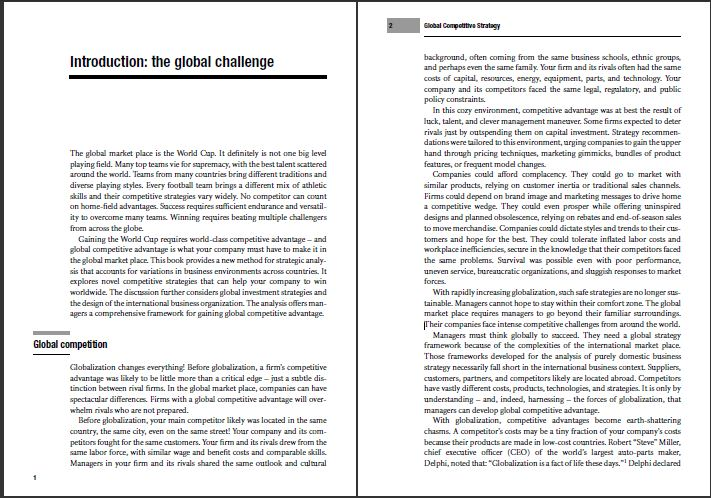
\includegraphics[width=0.8\textwidth]{chapter56}\vspace{0.5\baselineskip}
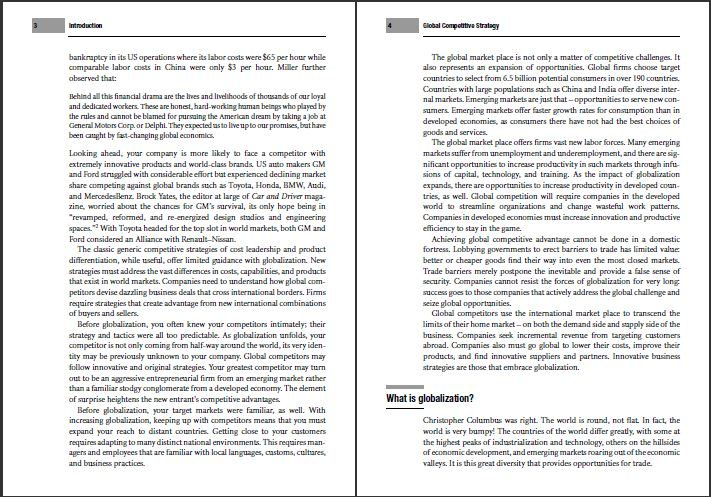
\includegraphics[width=0.8\textwidth]{chapter56a}
\caption{Example pages from \textit{Global Competitive Strategy}, by Daniel F. Spulber,} Cambridge University Press, 2007.
\label{globalstrategy}
\end{figure}

The interesting part of this design is that the headers as well as the chapter openings vary. On the even page the words ``Golbal Competitive Strategy'' are printed, which is the book title\footnote{Although it is an attractive design, it does not mean that this way of header information is a good way of structuring information.}.

Note that since LaTeX only provides two mark we need to arrange our own typesetting rules, we will abuse the macros to achieve it.

\begin{tcolorbox}
\begin{lstlisting}
\cxset{headings style56/.style={
          pagestyle=headings,
          header style=headings,
% Chaptermarks 
          chaptermark name color=black,
          chaptermark after number=,
          chaptermark name=SHORT BOOK TITLE,
          chaptermark numbering=none,
          chaptermark title color=black!80,
          chaptermark title before=\@gobble,
% Leftmarks
          leftmark before=\colorbox{thegray!50}{\thepage\quad}\quad, %even pages
          leftmark after=\hfill\hfill,
% Right marks influenced by chapter name?
          rightmark before=\colorbox{thegray!50}{\thepage\quad}\quad, %odd pages
          rightmark after=\hfill\hfill,
% Section marks
          sectionmark name custom=\chaptertitle@cx,
          sectionmark number=none,
          sectionmark name color=black,
          sectionmark title color=black!80,
          sectionmark before title=\@gobble, % we do not need the section title
          sectionmark after title=\hfill\hfill,
          sectionmark after number=,
%  rules we remove or inherit
%       header top rule=false,
          header bottom rule=true,
          header offset even=-1.3cm,
          header offset odd=-1.3cm,
          }}
\end{lstlisting}
\end{tcolorbox}

The approach we need to take here is to first define the even pages, which contain the book short title. Instead of printing the \cs{chaptername}, we give the value of the title to the \textbf{chaptermark} key.

\begin{tcolorbox}
   chaptermark name = SHORT BOOK TITLE,
\end{tcolorbox}

Offsetting the page numbers is done by using the \textbf{header offset} key. As both the left as well as the right pages have the page on the left we offset both of them by the same amount.

\begin{tcolorbox}
\begin{lstlisting}
    chaptermark name = SHORT BOOK TITLE,
    header offset even = -1.3cm,
    header offset odd  = -1.3cm,
\end{lstlisting}
\end{tcolorbox}

\subsection{Inheriting and transforming styles}
One of the advantages of this method, is that we can inherit styles and transform styles easily. Consider style57, which is shown in figure. This is a simple design and follows trends to include the book title in the header. This is a very similar design to header \textit{style57}.

\begin{tcolorbox}
\begin{lstlisting}
%% STYLE 57 QUANTUM FRONTIER
\cxset{headings style57/.style={
          headings style56,
% Chaptermarks 
          chaptermark name={\bfseries The Quantum Frontier},
% Leftmarks
          leftmark before=\thepage\quad, %even pages
          leftmark after=\hfill\hfill,
% Right marks influenced by chapter name?
          rightmark before=\hfill\hfill, %odd pages
          rightmark after=\thepage,
% Section marks
          sectionmark name custom=\chaptertitle@cx,
          sectionmark after title=\quad,
%  rules we remove or inherit
          header top rule=false,
          header bottom rule=false,
          header offset even=0pt,
          header offset odd=0pt,
          }}
\end{lstlisting}
\end{tcolorbox}

A crude form of object inheritance is possible by including a style at the top of the key definitions in this case \texttt{headings style56}, we then only need to redefine the values for the changes. We also set zero all offsets and adjust the widths. 

The success of the method is defining an appropriate set of general commands and building a community chest of styles. 

This concludes the long excursion into headers and footers. This class and method of styling is brand new and is bound to evolve, as it is being used. Feedback is most welcomed as well as bug reports.
\begin{figure}[tp]
\centering
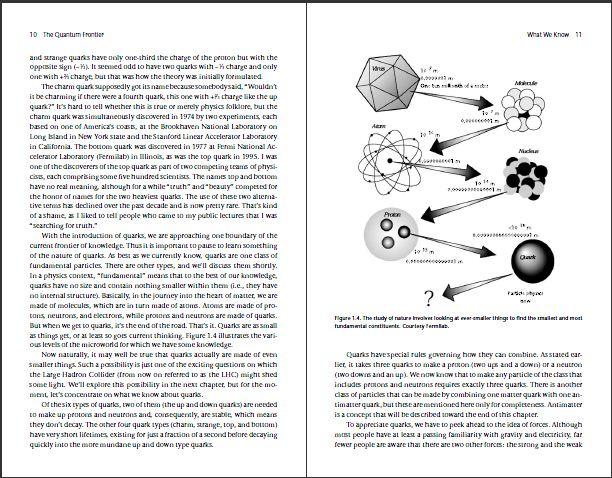
\includegraphics[width=0.8\textwidth]{chapter57a}\vspace{0.5\baselineskip}
\caption{Example pages from \textit{The quantum frontier: the large hadron collider}, by Don Lincoln, The Johns Hopkins University Press, 2009.  It uses the book short-title at even pages and the chapter title at the odd pages.}
\end{figure}

\section{Another inheritance example}

This example is from the book \textit{Evolution of the Insects} by David Grimaldi and Michael S. Engel and published by the Cambridge University Press in 2005. It is a beautifully typeset book and a fine piece of scientific work. The only difference in the headers of the previous examples is the setting of the page number and header text. This one as well as many other books uses the title of the book and the chapter name.

\begin{tcolorbox}
\begin{lstlisting}
%% EVOLUTION OF THE INSECTS
\cxset{headings style58/.style={
          headings style57,
          chaptermark name={\bfseries EVOLUTION OF THE INSECTS},
          leftmark before=\thepage\quad\hfill\hfill, %even pages
          leftmark after=,
          rightmark before=, %odd pages
          rightmark after=\hfill\hfill\thepage,
 }}
\end{lstlisting}
\end{tcolorbox}

Since most of the information was captured in \textit{style57} we inherit the values and only supply the ones  that are changing. This involves changing six settings, illustrating the strength of the procedure adopted. Just a word of caution I found it difficult to follow some of the terminology, if you confused by what a leftmark and right mark are think of them as holding all the header information except the page number.



\begin{figure}
\centering
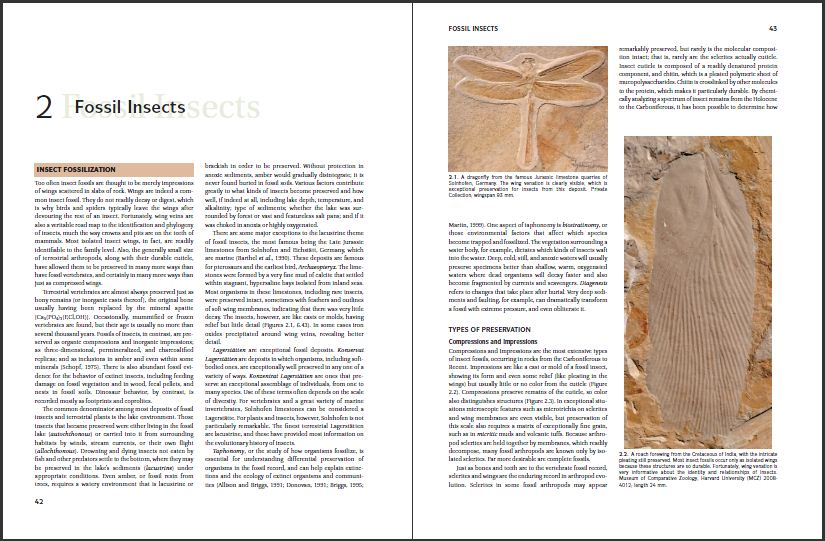
\includegraphics[width=0.8\textwidth]{chapter58}\vspace{0.5\baselineskip}
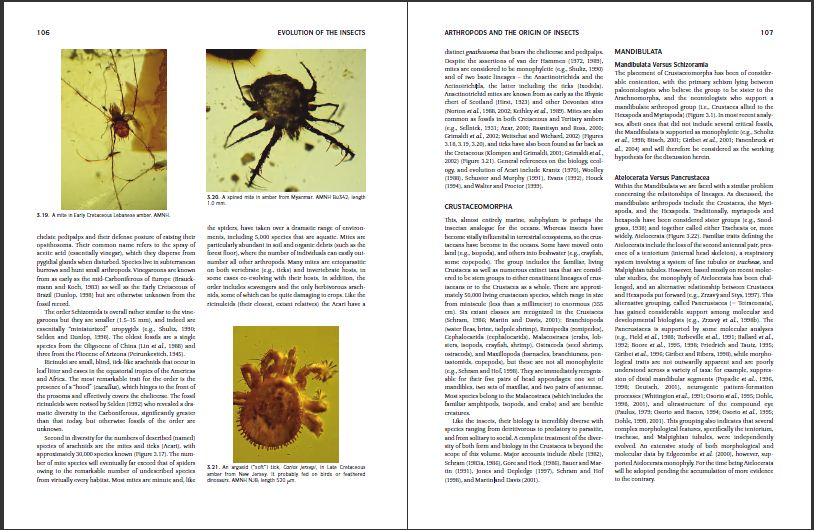
\includegraphics[width=0.8\textwidth]{chapter58a}
\caption{This example is from the book \textit{Evolution of the Insects}, David Grimaldi and Michael S. Engel,  Cambridge University Press, 2005. It is a beautifully typeset book and a fine piece of scientific work. The only difference in the headers of the previous examples is the setting of the page number and header text. This one as well as many other books use the title of the book and the chapter name in headers. The footers are empty with th exception of the chapter page}
\end{figure}


\begin{figure}
\centering
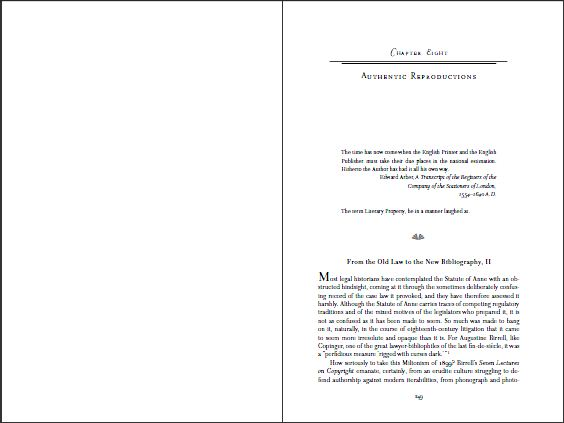
\includegraphics[width=0.8\textwidth]{chapter55}\vspace{0.5\baselineskip}
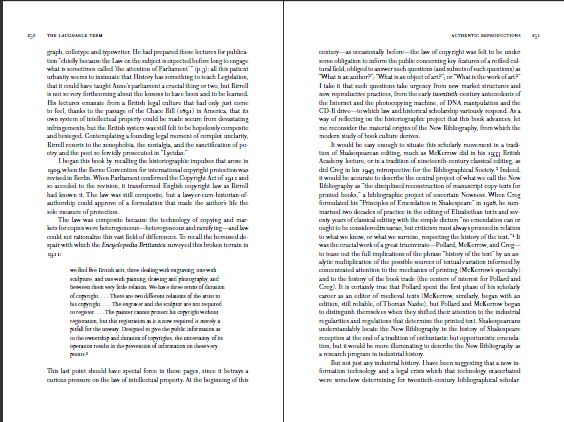
\includegraphics[width=0.8\textwidth]{chapter55a}
\caption{Example pages from \textit{The Author's Due, Printing and the Prehistory of Copyright}, by Joseph Lowewenstein, The University of Chicago Press, 2002.  It uses the part title on the even page and the chapter title on the odd page. The page number is set in the margin. The footers are clear.}
\end{figure}


\clearpage
\thispagestyle{empty}


%%%%%%%%%% NEW GEOMETRY
\newgeometry{top=1cm,bottom=2cm,left=2cm}

%% GENETICS
\@specialfalse
\cxset{
 custom=,
 name={CHAPTER CONCEPT},
 numbering=none,
 number font-size=,
 number font-family=,
 number font-weight=,
 number color=white,
 numbering=arabic,
 chapter opening=right,
 chapter color={black},
 chapter font-family=\sffamily,
 chapter font-size=\large,
 chapter font-weight=\bfseries,
 title font-family=\sffamily,
 title font-color=teal,
 rule off,
}

\begin{specialchapter}[
     image=genetics-dogs,
     image caption={Labrador retriever\\
         puppies expressing\\
         brown (chocolate),\\
         golden (yellow),\\
         and black\\
         coat colors,\\
         traits controlled\\
         by two gene pairs.}]%
{Extensions\\ of Mendelian\\ Genetics}
\begin{itemize}
\item While alleles are transmitted from parent to   offspring
according to Mendelian principles, they often do not
display the clear-cut dominant/recessive relationship
observed by Mendel.
\item In many cases, in a departure from Mendelian genetics,
two or more genes are known to influence the phenotype
of a single characteristic.
\item Still another exception to Mendelian inheritance occurs
when genes are located on the X chromosome, because one
of the sexes receives only one copy of that chromosome,
eliminating the possibility of heterozygosity.
\item Phenotypes are often the combined result of genetics and
the environment within which genes are expressed.
\item The result of the various exceptions to Mendelian principles
is the occurrence of phenotypic ratios that differ from those
produced by standard monohybrid, dihybrid, and trihybrid
crosses.
  \end{itemize}
\end{specialchapter}


%%%%%%%%%% NEW GEOMETRY
\newgeometry{top=2cm,bottom=2cm,left=2cm}
\clearpage

\begin{tcolorbox}
\begin{lstlisting}
%% Special Chapter command
\newcommand\specialchapter@cx[2][]{%
\refstepcounter{chapter}
\cxset{image/.store in=\image@cx,
       image caption/.store in=\caption@cx}
\cxset{#1}
\vbox to 0pt{\color{blue}\rule{\paperwidth}{0.4pt}\par\vskip-1.4pt
\rule{0.4pt}{\textheight}\rule{4cm}{0.4pt}}

\vbox to 0pt{\parbox[b]{4.7cm}{%
\raggedright

\leftskip1.5cm
\caption@cx\par
 \expandafter\rule{\rulewidth@cx}{5.8cm}
}\parbox[b]{0.5cm}{
\includegraphics[width=0.5cm,height=9.15cm]{./chapters/shadow}}\includegraphics{./chapters/\image@cx}\par}

\vspace{8.2cm}
\hspace*{-3.51cm}\hbox to 0pt{\hspace*{1.01cm}
\includegraphics[width=7.7cm,height=3.8cm]{./chapters/genetics-band}
\hspace*{-2.7cm}\sffamily\color{\numbercolor@cx}\HHUGE \raise30pt\hbox{\thechapter}%
\hspace{1.5cm}\raise0.5pt\hbox{
\includegraphics{./chapters/chapterconcept}
\includegraphics{./chapters/shadow2}}
}

%% Title name
\parbox[b]{0.45\textwidth}{%
  \titlefontsize@cx
  \titlefontweight@cx
  \titlefontfamily@cx
  \leftskip0.5em \color{\titlefontcolor@cx}
  #2
}
%% Concepts
}

\newenvironment{specialchapter}[2][]{%
  \if@openright\cleardoublepage\else\clearpage\fi
    \thispagestyle{plain}%
    \global\@topnum\z@
    \@afterindentfalse
    \specialchapter@cx[#1]{#2}
    \begin{minipage}{0.5\textwidth}%
    \vspace{0.5\baselineskip}
    \raggedright
}{\end{minipage}}
\end{lstlisting}
\end{tcolorbox}


The aim of the package is to allow easy styling of chapter heads and extends these to include images and special effects, which are difficult to achieve using traditional methods. 

Abstracting the various designs is a non-trivial undertaking due to the hundreds of different possibilities.

\begin{multicols}{2}
\long\def\specialsection#1{\hspace*{0.5em}\vbox{\hsize\columnwidth%
 \vspace{\baselineskip}
\refstepcounter{section}
\parindent0pt
\raggedright
\vbox to 0pt{%
\parindent0pt
\color{red}\rule[-49.6pt]{0.4pt}{50pt}%
\color{red}\rule{0.5in}{0.4pt}\colorbox{teal}{\color{white}{\large \space\thesection\space}}}%
\vskip5pt%
\hspace{-3.5pt}\fbox{.}\par
\vspace*{-45pt}
\hspace*{1em}\vbox{\Large\sffamily#1\par}}
\vspace*{\baselineskip}\par
}

\specialsection{The Ratio of Males to Females\\ in Humans is not 1.0}
\lipsum[2-5]
\specialsection{Variation in Chromosome Number:\\
Terminology and Origin}
\lipsum[1]
\bigskip
\noindent\textcolor{teal}{\large\bfseries\sffamily Monosomy}
\smallskip

\noindent\lipsum[2-3]


\specialsection{Background to the\\
sectioning commands}

The \LaTeX2e\ method of constructing the layout for Chapters is complicated and spread all over the book.cls code. Although not very difficult to customize, customization is not user friendly. 

\begin{description}
\item [counters] Counters can be displayed or not. These are constructed using the normal LaTeX method.
   \begin{verbatim}
   \renewcommand \thechapter {\@arabic\c@chapter}
   \end{verbatim}

\item [name] Here we use the term \textit{name} to denote in english the word ``chapter''. This can be typeset differently, depending on the language. It depends on on redefining one macro.
   \begin{verbatim}
     \def\chaptername{Chapter}
   \end{verbatim}
\item [openright] The global option open right, triggers the typesetting of chapter on odd pages only. There are a  couple of layouts that must be typeset on an even pages.

\item [\string\chapter] The chapter command is the main author command and where all the branching starts.
    \begin{verbatim}
\newcommand\chapter{%
  \if@openright\cleardoublepage\else\clearpage\fi
    \thispagestyle{plain}%
    \global\@topnum\z@
    \@afterindentfalse
    \secdef\@chapter\@schapter}
    \end{verbatim}

One limitation for this command is that it always starts a chapter on a new page and the macro needs to be rewritten if for example a new chapter is allowed to start anywhere.

Consider options openright, openleft, continuous.

The pagestyle is also settled here.

secdef will define basic macros for chaapter and starred chapter. What it basically does... this will become unecessary as we are going to find out a bit later on, but first the @chapter.

\item [\string\@chapter] This is the basic routine
\begin{verbatim}
\def\@chapter[#1]#2{
  \ifnum \c@secnumdepth >\m@ne
    \if@mainmatter
      \refstepcounter{chapter}%
      \typeout{\@chapapp\space\thechapter.}%
      \addcontentsline{toc}{chapter}%
         {\protect\numberline{\thechapter}#1}%
      \else
         \addcontentsline{toc}{chapter}{#1}%
    \fi
  \else
    \addcontentsline{toc}{chapter}{#1}%
  \fi
  \chaptermark{#1}%
  \addtocontents{lof}{\protect\addvspace{10\p@}}%
  \addtocontents{lot}{\protect\addvspace{10\p@}}%
  \if@twocolumn
    \@topnewpage[\@makechapterhead{#2}]%
  \else
    \@makechapterhead{#2}%
    \@afterheading
  \fi}
\end{verbatim}
  The important branching command here is makechapterhead,   which is responsible for typesetting the layout.

\end{description}
\end{multicols}


\section{Counters}
\begin{verbatim}
\renewcommand \thepart {\@Roman\c@part}
\renewcommand \thechapter {\@arabic\c@chapter}
\end{verbatim}



\section{major components}

The major components of a chapter opening, is the chapter name, the number and the title. It can be enclosed in boxes rules or other decorative elements. 

One peculiarity is how to specify the position of the number.

leftofchaptername rightofchaptername ownline 

\subsection{algorithmic approach}

The strategy in abstracting the chapter commands follows closely to that of laTeX.

First the chapter is called with the minimum of redefinitions. This then calls makechapterhead.


\begin{specialchapter}[
     image=genetics-dogs,
     image caption={Labrador retriever\\
         puppies expressing\\
         brown (chocolate),\\
         golden (yellow),\\
         and black\\
         coat colors,\\
         traits controlled\\
         by two gene pairs.}]%
{Sample\\ Chapter\\ Styles}
\begin{itemize}
\item The many permutations of variables affecting a chapter design, necessitate an interface that is easy to use and remember. The package provides an interface that a design can simply be changed by changing one word.
\item Learn how to select from a number of predefined styles, which you can view in the pages that follow.
\item Learn how to design your own styles and incorporate them easily in a new document.
\item The designs that follow have been selected from actual books. They may differ slightly in page geometry, spacing and fonts as I have tried to keep a somewhat unified design across this document.
\item i welcome contributions in terms of libraries and additional styles. What I have provided in this package is only a very small subset of what is possible to achieve.
\item Almost all styles are numbered, as this was the easiest way to incorporate so many designs. The few exceptions are noted in the relevant pages.
  \end{itemize}
\clearpage
\end{specialchapter}


%%%%%%%%%%%%%%%%%%%%%%%%%%%%%%%%%%%%%%%%%%%%%%%%%%%%%
%%%%%%%%%  GENERAL SETTINGS
\cxset{steward,
  chapter toc=true,
  numbering=arabic,
  custom=tikzspecial,
  offsety=0cm,
  image=hine03,
  texti={When Lamport designed the original \LaTeX\ sectioning commands, limitations of computer power forced him to restrict the abstraction of complicated chapter layouts. With current tools available improvements are much easier to program.},
  textii={In this chapter we discuss a method that allows the production of fancy chapter headings and formatting, based on a set of key values. Central  to this process is the separation of content from presentation.
We also discuss the basic formatting tools that are available and how one can modify them to mould new book designs.},
}
\@specialtrue

\cxset{chapter opening=left}

\chapter{General Settings}

\section{Introduction}

Here we define and set general paragraph settings. The parameters which control \TeX's behaviour when typesetting paragraphs can receive a bit of a tweak here. We also describe a set of options to handle parameters that can influence grid typesetting. This is especially important for two or more column typesetting.

\subsection{Parameters controlling paragraphs}\index{Paragraphs!controlling parameters}
The parameters \cs{lineskip} and \cs{normallineskip} influence \TeX\ when two lines come two close.
\medskip

\keyval{lineskip}{\marg{dim}}{Lineskip parameter}
\keyval{normallineskip}{\marg{dim}}{Lineskip parameter.}
\keyval{lineskiplimit}{\marg{number}}{Lineskip limit}
\keyval{parindent}{\marg{dim}}{Paragraph indentation.}
\keyval{text-indent}{\marg{dim}}{Alias for \cs{parindent}.}
\keyval{parskip}{\marg{dim}}{Spacing between paragraphs.}

\cxset{lineskip/.code=\setlength\lineskip{#1},
          normallineskip/.code=\setlength\normallineskip{#1},
          parindent/.code=\setlength\parindent{#1},
          parskip/.code=\setlength\parskip{#1},
          text-indent/.code=\setlength\parindent{#1},
          baselinestretch/.code=\renewcommand\baselinestretch{#1}}

\renewcommand*{\linenottooshort}[1][4em]{%
  \@tempdima=\hsize
 \advance\@tempdima-#1
 \leftskip0pt
 \rightskip\leftskip
\parfillskip\@tempdima\@minus\@tempdima
}
\renewcommand*{\lastlineparrule}{%
  \hrule height 0.5ex depth \@tempdimb\relax}

\renewcommand*{\lastlinerulefill}{%
  \let\\\@centercr
  \@tempdimb=-0.5ex \advance\@tempdimb 0.4pt
  \unskip\nobreak\space
  \leaders\lastlineparrule\hskip\@flushglue
  \vadjust{}{\parfillskip\z@\@@par}}%check this out
\begin{example}{Paragraph parameters, using CSS style commands}{}
\cxset{lineskip=1pt,
          normallineskip=1pt,
          parindent=1em}

\lipsum[1]

\cxset{
          lineskip=2pt,
          normallineskip=2pt,
          parindent=1.5em,
          parskip=3pt,
          baselinestretch={},
 }
\linenottooshort[20em]

\lipsum[1-2]
\lorem

\end{example}

These command offer little value over the normal \TeX\ macros other than keeping the interface, uniform. One can also extend the interface to cover CSS style commands:

\begin{example}{Paragraph parameters}{}
\cxset{text-indent=50pt}
\vbox to 4cm{\lipsum*[1]}
\end{example}

Another advantage, the package offers a few pre-configured styles, just setting a style to latex will revert everything back to latex.

\section{Technical discussion}

Most classes, including the standard \LaTeXe\ classes as well as packages attempting to achieve a grid typesetting try define a text height that is a multiple of \cs{baselineskip}. This way they give little opportunity to TeX to adjust the vertical glue to achieve a flush bottom.

\subsection{Grid typesetting}
\the\textheight

\begin{tcolorbox}{title= Grid type typesetting}
%\begin{lstlisting}
\def\Grid@baseline{10\p@}
\def\Grid@fontsize{12\p@}
\def\Grid@lines{40}
\def\Grid@textheight{%
       \@tempdima=\Grid@baseline%
       \multiply\@tempdima by \Grid@lines%
       \textheight=\the\@tempdima%
}
\Grid@textheight
\renewcommand\normalsize{%
   \baselineskip=\Grid@baseline%
   \@setfontsize\normalsize{\Grid@fontsize}{\Grid@baseline}%
   \lineskip=0pt
   \lineskiplimit=-\Grid@fontsize%
   \abovedisplayskip \baselineskip%
   \abovedisplayshortskip .5\baselineskip%
   \belowdisplayskip \abovedisplayskip
   \belowdisplayshortskip \abovedisplayshortskip
   \let\@listi\@listI}
\normalsize
%\end{lstlisting}
\end{tcolorbox}
\newdimen\floatunit
\newskip\allfloats
\setlength\floatunit{\the\baselineskip}

\setlength\allfloats{\floatunit}

\setlength\floatsep{\allfloats}
\setlength\textfloatsep{\allfloats}
\setlength\intextsep{\allfloats}
\setlength\dblfloatsep{\allfloats}
\setlength\dbltextfloatsep{\allfloats}

\setlength\@fptop{\z@}
\setlength\@fpsep{\z@}
\setlength\@fpbot{\z@}
\setlength\@dblfptop{\z@}
\setlength\@dblfpsep{\z@}
\setlength\@dblfpbot{\z@}

\begingroup
  \catcode`P=12
  \catcode`T=12
  \lowercase{
    \def\x{\def\rem@decimal##1.##2PT{##1}}}
  \expandafter\endgroup\x
\def\strip@decimal{\expandafter\rem@decimal\the}

\begingroup
  \catcode`P=12
  \catcode`T=12
  \lowercase{
    \def\y{\def\rem@dot##1.##2PT{##1##2}}}
  \expandafter\endgroup\y
\def\strip@dot{\expandafter\rem@dot\the}

\newdimen\halfbaselineskip
\halfbaselineskip=\floatunit
\divide\halfbaselineskip by 2

\newdimen\figboxht

\long\def\roundoff{\figboxht=\fight%
    \advance\figboxht by \baselineskip%
    \multiply\figboxht by 10%
    \xdef\xbaselineskip{\strip@dot\baselineskip}%
    \divide\figboxht by \xbaselineskip%
    \xdef\mylines{\strip@decimal\figboxht}%
    \figboxht=\baselineskip%
    \multiply\figboxht by\mylines%
    \advance\figboxht -\fight%
    \ifdim\the\figboxht>\the\halfbaselineskip%
      \advance\figboxht by -\floatunit%
    \else\fi%
    }
%%%
%%  Floats
%
%\let\oldfigure\figure
%\let\oldendfigure\endfigure
%\expandafter\let\csname oldfigurest\expandafter%
%              \endcsname\csname figure*\endcsname
%\expandafter\let\csname oldendfigurest\expandafter%
%              \endcsname\csname endfigure*\endcsname
%
%\let\oldtable\table
%\let\oldendtable\endtable
%\expandafter\let\csname oldtablest\expandafter%
%              \endcsname\csname table*\endcsname
%\expandafter\let\csname oldendtablest\expandafter%
%              \endcsname\csname endtable*\endcsname
%
%\renewenvironment{figure}
%         {\oldfigure\begin{gridfltenv}}
%         {\end{gridfltenv}\oldendfigure}
%\renewenvironment{figure*}
%         {\oldfigurest\begin{gridfltenv}}
%         {\end{gridfltenv}\oldendfigurest}
%
%\renewenvironment{table}
%         {\oldtable\begin{gridfltenv}}
%         {\end{gridfltenv}\oldendtable}
%\renewenvironment{table*}
%         {\oldtablest\begin{gridfltenv}}
%         {\end{gridfltenv}\oldendtablest}
%
%\newenvironment{gridfltenv}
%         {\global\setbox0=\vbox\bgroup}
%         {\egroup%
%          \xdef\fight{\the\ht0}%
%          \roundoff%
%          \leavevmode\vadjust{\box0\vskip\figboxht}\hfil\break%
%         }
%
%%%%
%%%  Equations
%%
%\newenvironment{gridenv}
%         {\global\setbox0=\vbox\bgroup}
%         {\egroup%
%          \xdef\fight{\the\ht0}%
%          \roundoff%
%          \leavevmode%
%          \vadjust{\vskip0.5\figboxht%
%                   \box0%
%                   \vskip0.5\figboxht%
%                   }\hfil\break%%
%         }

\jot=\baselineskip

\begin{multicols}{2}
\parskip 0pt\normalsize
\lipsum[1-4]
This is some test\par

\vskip \baselineskip 
{\hfil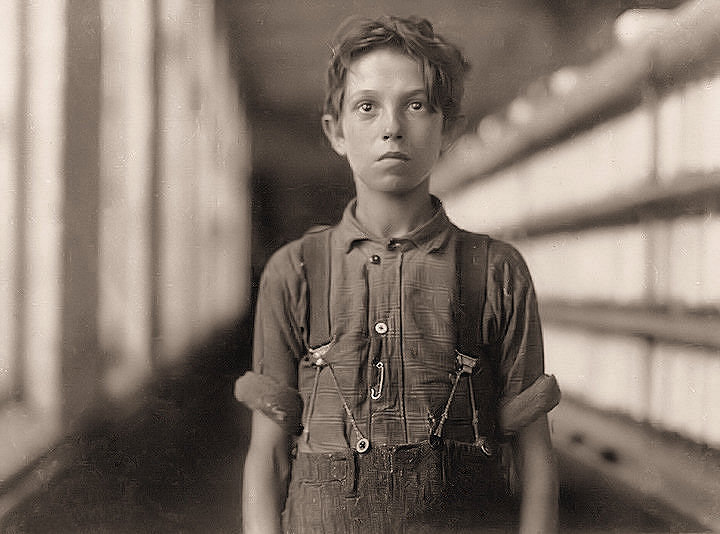
\includegraphics[height=203.5pt, width=5cm, keepaspectratio]{hine02}\hfill}
\vskip1pt 
\vskip\baselineskip
\lipsum[1-10]\lipsum
\end{multicols}
\the\textheight\\
\the\paperheight


%%%%%%%%%%%%%   END GENERAL SETTINGS  %%%%%%%%%%%%%%%%%%%%%%%
\clearpage
\@specialfalse
%% EDDOUARD MANET
\cxset{manet/.style={
 chapter opening=anywhere,
 chapter toc=true,
 toc image=false,
 name={},
 numbering=none,
 number font-size=,
 number font-family=,
 number font-weight=,
 number before={\vspace*{-2.5cm}},
 number dot={},
 number after={},
 number position=leftname,
 chapter font-family=,
 chapter font-weight=,
 chapter font-size=,
 chapter before={},
 chapter after={},
 chapter color={black!90},
 number color=\color{purple},
 title beforeskip={},
 title afterskip={},
 title before={\hskip-2.3cm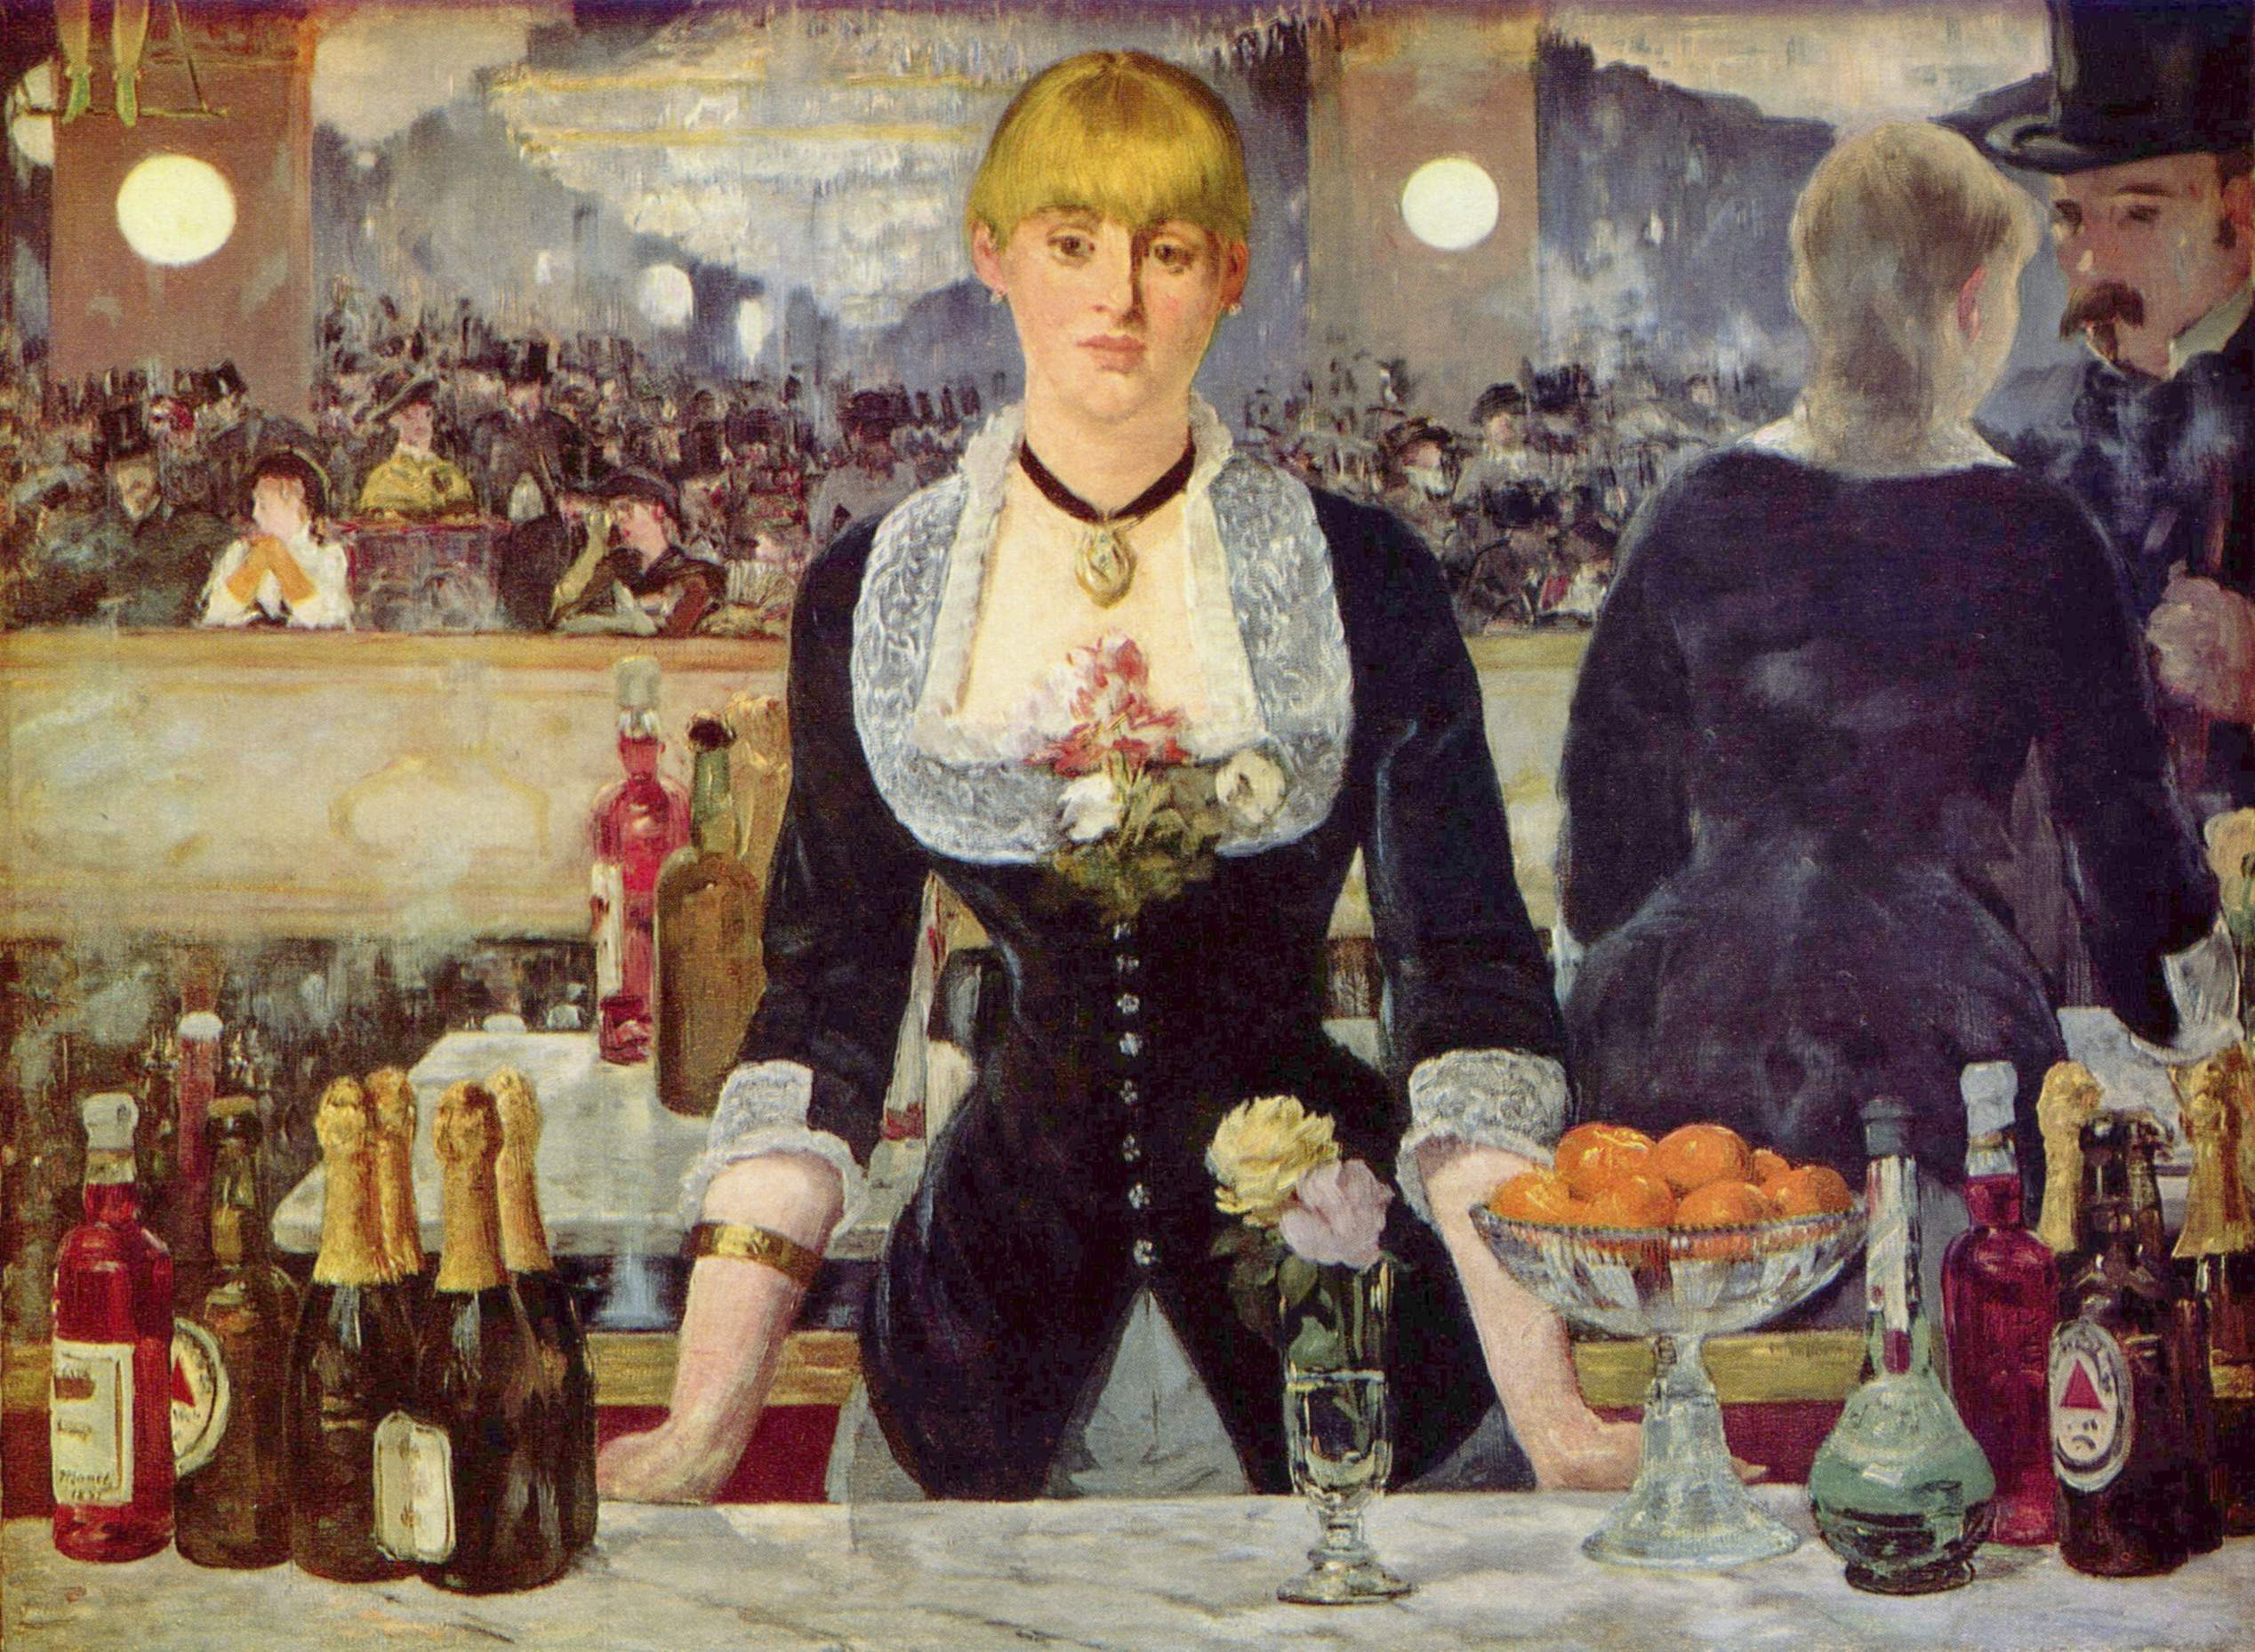
\includegraphics[width=1.25\textwidth]{./chapters/manet}\par
    \par\hfill\hfill{\tiny\bfseries Manet's  \textit{The Barmaid.}}\\
    \par
    \vspace*{\baselineskip}
    \par\hfill},
 title after={\hfill\hfill},
 title font-family=\sffamily,
 title font-color=\color{black!80},
 title font-weight=\bfseries,
 title font-size=\LARGE}}

% need to reset 

\cxset{manet, toc image=true}
\chapter{EDOUARD MANET}
\begin{multicols}{3}
      \leftskip0pt
      \lettrine{I}{psum dolor} sit amet latixeus. \lipsum*[1-2]
      Latinicus porcupinus to fill the line.
\end{multicols}


%% CARDINAL
\cxset{toc image=false},
\cxset{manet}

\def\topimage#1{\cxset{title before={\hskip-2.3cm\includegraphics[width=1.25\textwidth]{./chapters/#1}\par
\vspace*{\baselineskip}\par}}}


\cxset{manet}
\cxset{toc image=false},
\topimage{Alan-MacDonald-Cardinal-Spin-01}

\chapter{ALAN MacDONALD}
\begin{multicols}{3}
      \leftskip0pt
      \lettrine{I}{psum dolor} sit amet latixeus. \lipsum*[1-2]
      Latinicus porcupinus to fill the line.
\end{multicols}
\clearpage

\cxset{manet,toc image=false}
\topimage{Alan-MacDonald-Cardinal-Spin-01}

\chapter{A New Approach to Designing \LaTeX\ Classes}
\begin{multicols}{3}
      \leftskip0pt
      \lettrine{I}{psum dolor} sit amet latixeus. \lipsum*[1-2]
      Latinicus porcupinus to fill the line.
\end{multicols}
\clearpage



This particular code, uses the predefined style \textit{manet}. The only difference we have now defined a helper macro to make it easier for such images to be inserted for similar style chapter openings.

\medskip

\begin{lstlisting}
\def\topimage#1{\cxset{title before={\hskip-2.3cm\includegraphics[width=1.25\textwidth]{./chapters/#1}\par
\vspace*{\baselineskip}\par}}}
\end{lstlisting}

If a full book is to be designed using chapter openings in this fashion more keys and styles could be defined to make it even more easy to enter.

The full code to have the chapter typeset is shown below:
\medskip

\begin{lstlisting}
\cxset{manet}
\topimage{Alan-MacDonald-Cardinal-Spin-01}

\chapter{ALAN MacDONALD}
\begin{multicols}{3}
      \leftskip0pt
      \lettrine{I}{psum dolor} sit amet latixeus. \lipsum*[1-2]
      Latinicus porcupinus to fill the line.
\end{multicols}
\end{lstlisting}
\lipsum[2]

\cxset{toc image=false},

%% STYLE PICTURE IN OPENING PAGE
\long\gdef\versochapter#1{%
  \vspace*{3cm}
  \minipage{\textwidth}
  \hfill\includegraphics[width=0.63\textwidth]{\chapterimage@cx}\par
  \vspace*{6pt}
  \hfill\minipage{0.75\textwidth}
  {\HUGE\bfseries\flushright #1\endflushright}
  \endminipage
  \endminipage
  \newpage
 
% for recto page
\vspace*{10cm}
\@specialfalse
\@openleftfalse
\@openanyfalse
\@openrighttrue
}
%customedesign@cx

\newgeometry{bottom=2.5cm}

\cxset{
   chapter image/.code={\def\chapterimage@cx{#1}},
   chapter opening/.is choice,
   chapter opening/verso/.code={\@specialtrue\@openlefttrue
   \gdef\customdesign@cx##1{\versochapter{##1}}}
}

\cxset{
 chapter image=onesowndeath,
 chapter opening=verso,
 name={},
 numbering=none,
 number font-size=\LARGE,
 number font-family=\rmfamily,
 number font-weight=\bfseries,
 number before=,
 number dot=,
 number after=,
 number position=leftname,
 chapter font-family=\sffamily,
 chapter font-weight=\normalfont,
 chapter font-size=\Large,
 chapter before={\vspace*{0pt}\par},
 chapter after={\hfill\hfill\par},
 chapter color={black!90},
 number color=\color{purple},
 title beforeskip={\vspace*{0pt}},
 title afterskip={\vspace*{0.4\textheight}\par},
 title before={},
 title after={},
 title font-family=\sffamily,
 title font-color=\color{purple},
 title font-weight=\bfseries,
 title font-size=\LARGE,
 header style=plain,
 pagestyle=plain,
 }

\@specialtrue

\chapter[VERSO CHAPTERS]{Verso Chapters}

\parindent1.5em
{\HUGE V}erso chapter openings are not common. One design that I found quite attractive is \lipsum[1-3] \textit{From Western attitudes toward death from the middle ages to the present}, Philippe Ari\'es. London, 1974.

\begin{figure}
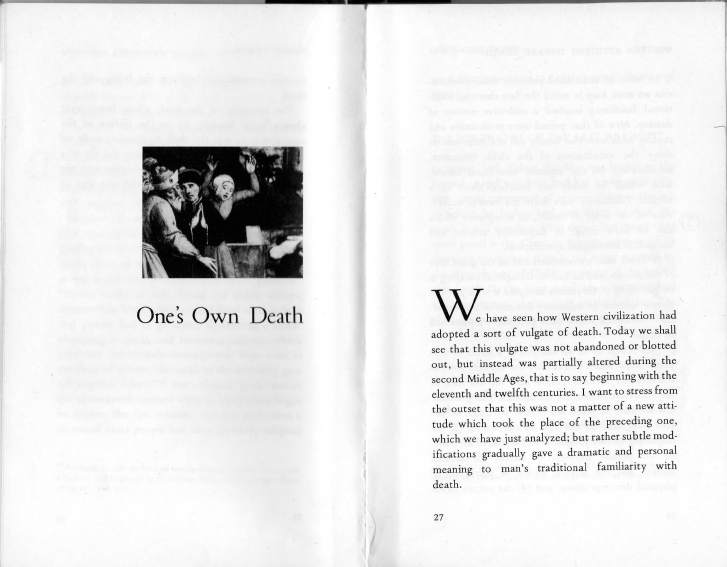
\includegraphics[width=\textwidth]{versochapter01}
\caption{Chapter opening on verso page.}
\end{figure}



\cxset{chapter image=tameddeath,
         chapter opening=verso,
         header style=empty,
         pagestyle=empty}

\chapter[VERSO CHAPTERS]{Verso Chapters}
\lipsum


\@specialfalse
%%%%%%%%%%%%%%%%%%%%%%%%%%%%%%%%%%%%%%%%%%%
%%%%%%  STYLE 01
%%%%%%%%%%%%%%%%%%%%%%%%%%%%%%%%%%%%%%%%%%%


\cxset{
 name={},
 numbering=arabic,
 number font-size=\LARGE,
 number font-family=\rmfamily,
 number font-weight=\bfseries,
 number before=,
 number dot=,
 number after=,
 number position=leftname,
 chapter font-family=\sffamily,
 chapter font-weight=\normalfont,
 chapter font-size=\Large,
 chapter before={\vspace*{20pt}\par},
 chapter after={\hfill\hfill\par},
 chapter color={black!90},
 number color=\color{purple},
 title beforeskip={\vspace*{30pt}},
 title afterskip={\vspace*{40pt}\par},
 title before={},
 title after={},
 title font-family=\sffamily,
 title font-color=\color{purple},
 title font-weight=\bfseries,
 title font-size=\LARGE,
 header style=headings}

\cxset{headings ruled-01}

\chapter{Introduction to Style One}


\begin{summary}
This design is simple and its distinguishing characteristic is a short summary at the beginning of the chapter. This is almost like an abstract typeset in italic font without setting the margins in. We provide a \lstinline{summary} environment for convenience. Note the very simple line in the running head to the left of the page number.
\end{summary}

\medskip
\begin{figure}[ht]
\centering
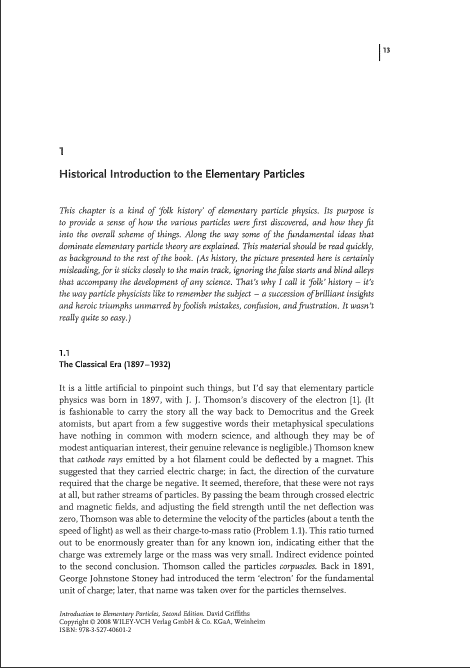
\includegraphics[width=0.5\textwidth]{./chapters/chapter01}
\end{figure}






%%%%%%%%%%%%%%%%%%%%%%%%%%%%%%%%%%%%%%%%%%%
%%%%%%  STYLE 02
%%%%%%%%%%%%%%%%%%%%%%%%%%%%%%%%%%%%%%%%%%%
\clearpage

\cxset{
 name={},
 numbering=arabic,
 number font-size=\LARGE,
 number font-family=\rmfamily,
 number font-weight=\bfseries,
 number before=,
 number dot=.,
 number after=\hspace{1em},
 number position=rightname,
 chapter font-family=\sffamily,
 chapter font-weight=\normalfont,
 chapter font-size=\Large,
 chapter before={\vspace*{20pt}\par\hfill},
 chapter after={},
 chapter color={black!90},
 number color=\color{purple},
 title beforeskip={},
 title afterskip={\vspace*{50pt}\par},
 title before={},
 title after={},
 title font-family=\sffamily,
 title font-color=\color{purple},
 title font-weight=\bfseries,
 title font-size=\LARGE}

\chapter{Style 2}
\parindent0pt
I tend to favour this design for books that have a lot of pictures. It brings the design into the margins and leaves plentiful white space in the margins. From a programming point of view the chapter is the opposite of openany. It has to open on an odd number.
\medskip
\begin{figure}[ht]
\centering
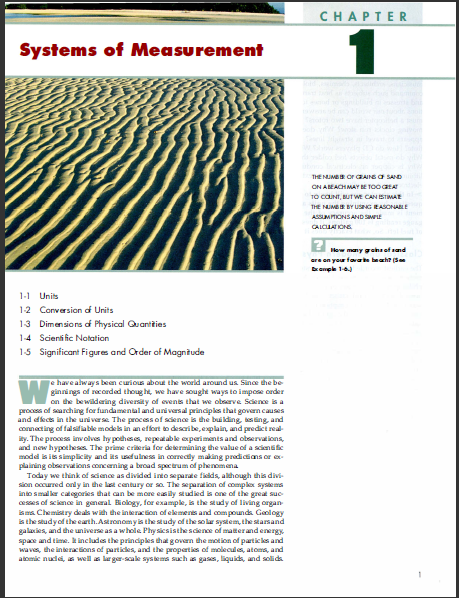
\includegraphics[width=0.6\textwidth]{./chapters/chapter02}
\end{figure}



%%%%%%%%%%%%%%%%%%%%%%%%%%%%%%%%%%%%%%%%%%%
%%%%%%  STYLE 03
%%%%%%%%%%%%%%%%%%%%%%%%%%%%%%%%%%%%%%%%%%%
\newgeometry{top=-10pt,bottom=2cm}
\tcbset{width=\paperwidth,boxrule=0pt,right=3cm,arc=0pt}

\cxset{style03/.style={
 name={},
 numbering=arabic,
 number font-size=\HUGE,
 number font-family=\rmfamily,
 number font-weight=\bfseries,
 number before=,
 number dot=.,
 number after=,
 number position=rightname,
 chapter font-family=\sffamily,
 chapter font-weight=\normalfont,
 chapter font-size=\Large,
% start colorbox
 chapter before={\hspace*{-2.5cm}\vbox\bgroup\tcolorbox\bgroup\vspace*{20pt}\hfill\hfill},
 chapter after={\par\vspace*{15pt}},
 chapter color={black!90},
 number color=\color{purple},
 title beforeskip={},
 title afterskip={\vspace*{10pt}\par},
 title before={\hfill\hfill},
% end colorbox
 title after={\vspace*{60pt}\egroup\endtcolorbox\egroup},
 title font-family=\sffamily,
 title font-color=\color{purple},
 title font-weight=\bfseries,
 title font-size=\Huge}}

\cxset{style03}

\chapter{Introduction Style Three}

This is not an exact reproduction as I am still thinking as to how to use
specials with the package. You can vary it by setting the tcolorbox settings as well as the geometry settings.
\medskip
\begin{figure}[ht]
\centering

\includegraphics[width=0.39\textwidth]{./chapters/chapter03}
\end{figure}

This setting involves changing the geometry of the page as well as adding the chapter name and title in a color box. For this I have used the \lstinline{tcolorbox}. Of course you can use any other shaded environment you feel comfortable with such as mdframed. It is important to set the colorbox parameters.

\begin{lstlisting}
\newgeometry{top=-10pt}
\tcbset{width=\paperwidth,boxrule=0pt,right=3cm,arc=0pt}
\end{lstlisting}

Note that we set the width of the \lstinline{tcolorbox} to \lstinline{\paperwidth} in order for the shading to extend to the full width of the page.

\restoregeometry

%%%%%%%%%%%%%%%%%%%%%%%%%%%%%%%%%%%%%%%%%%%
%%%%%%  STYLE 04
%%%%%%%%%%%%%%%%%%%%%%%%%%%%%%%%%%%%%%%%%%%
\clearpage
\cxset{style04/.style={
 name={},
 numbering=Roman,
 number font-size=\Large,
 number font-family=\rmfamily,
 number font-weight=\bfseries,
 number before=,
 number dot=,
 number after=,
 number position=rightname,
 chapter font-family=\rmfamily,
 chapter font-weight=\normalfont,
 chapter font-size=\Large,
 chapter before={\vspace*{20pt}\par\hfill},
 chapter after={\hfill\hfill\par\vspace*{10pt}},
 chapter color={black!90},
 number color=\color{purple},
 title beforeskip={},
 title afterskip={\vspace*{50pt}\par},
 title before={\hfill},
 title after={\hfill\hfill\par},
 title font-family=\rmfamily,
 title font-color=\color{purple},
 title font-weight=\normalfont,
 title font-size=\LARGE}}

\cxset{style04}

\chapter{INTRODUCTION TO STYLE FOUR}

This is a very simple design applicable perhaps to translations and commentary on older texts.
\medskip
\begin{figure}[ht]
\centering
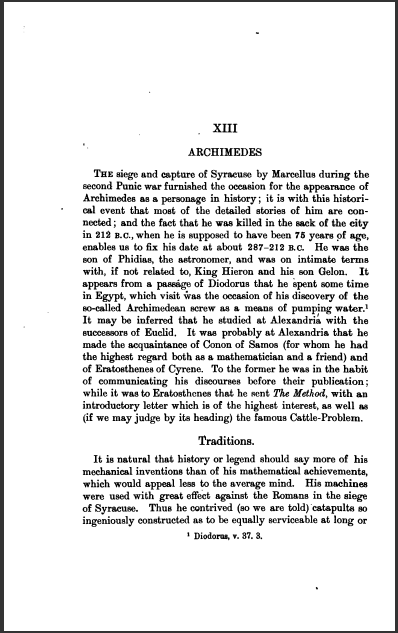
\includegraphics[width=0.6\textwidth]{./chapters/chapter04}
\end{figure}


%%%%%%%%%%%%%%%%%%%%%%%%%%%%%%%%%%%%%%%%%%%
%%%%%%  STYLE 05
%%%%%%%%%%%%%%%%%%%%%%%%%%%%%%%%%%%%%%%%%%%


\cxset{style05/.style={
 name={Chapter},
 numbering=arabic,
 number font-size=\Large,
 number font-family=\rmfamily,
 number font-weight=\normalfont\itshape,
 number color=\color{black!90},
 number before=,
 number dot=,
 number after=,
 number position=rightname,
 chapter font-family=\rmfamily,
 chapter font-weight=\normalfont\itshape,
 chapter font-size=\Large,
 chapter before={\hrule width \columnwidth \kern2.6\p@ \par\hfill},
 chapter after={\hfill\hfill\par},
 chapter color={black!90},
 chapter spaceout=none,
 title beforeskip={\vspace*{10pt}},
 title afterskip={\vspace*{50pt}\par},
 title before={\hfill},
 title after={\hfill\hfill \vskip2.6pt\hrule width \columnwidth \kern2.6\p@ },
 title font-family=\sffamily,
 title font-color=\color{black!90},
 title font-weight=\bfseries,
 title font-size=\huge,
 header style=empty}}

\cxset{style05}
\chapter{Introduction to Style Five}\index{ch:style5}

\tcbset{width=\textwidth}
I think this style can be improved with a bit of color. You can experiment with it quite easily. The spacing on top of this style can also be adjusted to suit your typographical taste.
\medskip
\begin{figure}[ht]
\centering
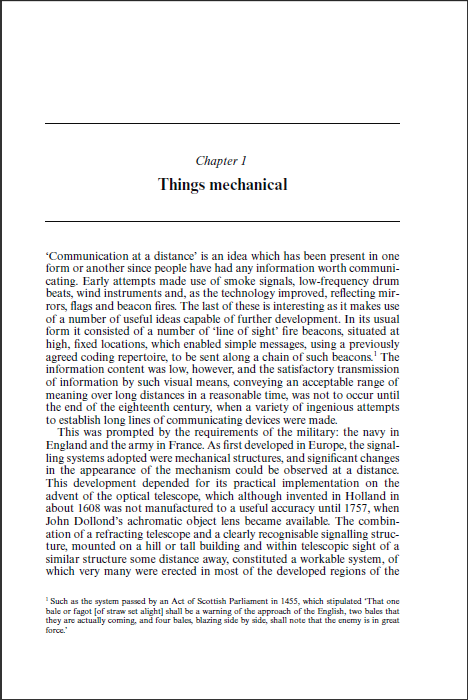
\includegraphics[width=0.6\textwidth]{./chapters/chapter05}
\end{figure}

\section{General notes on rules}

LaTeX's default rules would normally give problems. Best is to use TeX's primitives to built them.

\index{rules!example color}
\begin{texexample}{}{}
\hrule width 5cm \kern2.6\p@   
AAAAAAAAAAAAAAAAAAAAA
\vskip2.6pt\hrule width 5cm 
\medskip

Problem with LaTeX rules.

\rule{5cm}{0.4pt}\par  
AAAAAAAAAAAAAAAAAAAAA\par%
\rule[6.5pt]{5cm}{0.4pt} 

\def\rule{\@ifnextchar[\@rule{\@rule[\z@]}}
\def\@rule[#1]#2#3{%
 \leavevmode
 \hbox{%
 \setlength\@tempdima{#1}%
 \setlength\@tempdimb{#2}%
 \setlength\@tempdimc{#3}%
 \advance\@tempdimc\@tempdima%
 \vrule\@width\@tempdimb\@height\@tempdimc\@depth-\@tempdima}}

\def\thickrule{\leavevmode \leaders \hrule height 3pt \hfill \kern \z@}

{\color{teal}\hrule width 10.5cm height3pt \kern2.6\p@ 
    {{\color{black!80}\HUGE CHAPTER TITLE}}\vskip3pt
\hrule width 10.5cm height3pt}
\end{texexample}


\end{document}
%%%%%%%%%%%%%%%%%%%%%%%%%%%%%%%%%%%%%%%%%%%
%%%%%%  STYLE 06
%%%%%%%%%%%%%%%%%%%%%%%%%%%%%%%%%%%%%%%%%%%

\cxset{style6/.style={
 name={Chapter},
 numbering=arabic,
 number font-size=\Huge,
 number font-family=\rmfamily,
 number font-weight=\calligra,
 number color=\color{black!90},
 number before=\kern-4.5pt,
 number dot=,
 number after=,
 number position=rightname,
 chapter font-family=\rmfamily,
 chapter font-weight=\normalfont\itshape,
 chapter font-size=\LARGE\calligra,
 chapter before={\vspace*{20pt}\par\hfill},
 chapter after={\hfill\hfill\par},
 chapter color={black!90},
 title beforeskip={\vspace*{50pt}},
 title afterskip={\vspace{20pt}\par},
 title before={\hfill},
 title after={\hfill\hfill},
 title font-family=\rmfamily,
 title font-color=\color{black!90},
 title font-weight=\normalfont,
 title font-size=\LARGE,
 title spaceout=soul,
}}

\cxset{style6}

\chapter{INTRODUCTION TO STYLE SIX}

The calligraphic font for this design make it stand out, although you may need to experiment to get the right font (I have used calligra). I am sure the specification can be optimized a bit, however so far it works. I also opted to space out the title.
\medskip
\begin{figure}[ht]
\centering
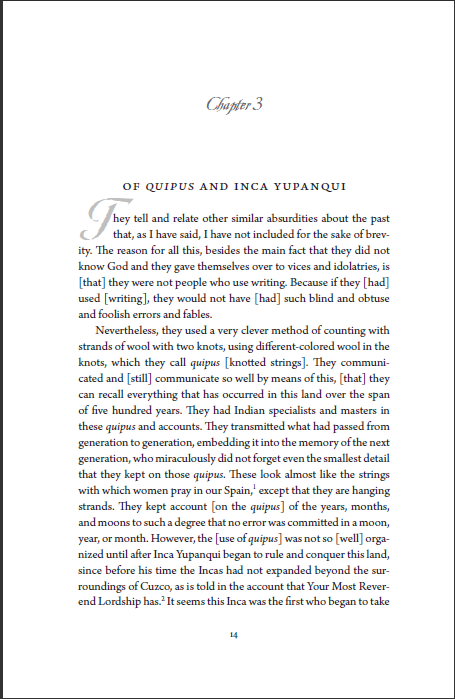
\includegraphics[width=0.6\textwidth]{./chapters/chapter06}
\end{figure}

The number has been kerned using:

\begin{lstlisting}
 number before=\kern-4.5pt,
\end{lstlisting}


\newgeometry{top=2cm,bottom=2cm,left=3cm,right=3cm}
%%%%%%%%%%%%%%%%%%%%%%%%%%%%%%%%%%%%%%%%%%%
%%%%%%  STYLE 07
%%%%%%%%%%%%%%%%%%%%%%%%%%%%%%%%%%%%%%%%%%%

\cxset{style7/.style={
 name={},
 numbering=arabic,
 number font-size=\Huge,
 number font-family=\rmfamily,
 number font-weight=\bfseries,
 number before=,
 number dot=,
 number color=\color{gray},
 number after=\par,
 number position=rightname,
 chapter font-family=\sffamily,
 chapter font-weight=\normalfont,
 chapter font-size=\Large,
 chapter before={\hfill\hfill\par},
 chapter after={},
 chapter color={black!90},
 title beforeskip={\vspace*{30pt}},
 title afterskip={\vspace*{50pt}\par},
 title before={},
 title after={\par\rule[13pt]{\textwidth}{0.4pt}},
 title font-family=\sffamily,
 title font-color=\color{purple},
 title font-weight=\bfseries,
 title font-size=\LARGE,
 title spaceout=none,
}}

\cxset{style7}
\chapter{Introduction to Style Seven}

\parindent0pt
\lipsum[1]
\medskip
\begin{figure}[ht]
\centering
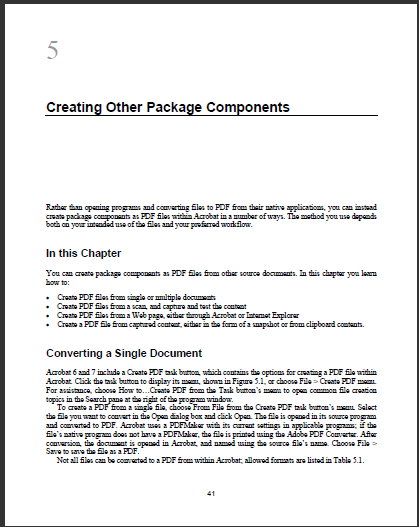
\includegraphics[width=0.6\textwidth]{./chapters/chapter07}
\end{figure}
\lipsum[1]


%%%%%%%%%%%%%%%%%%%%%%%%%%%%%%%%%%%%%%%%%%%
%%%%%%  STYLE 08
%%%%%%%%%%%%%%%%%%%%%%%%%%%%%%%%%%%%%%%%%%%
\clearpage

\cxset{style8/.style={
 name={},
 numbering=arabic,
 number font-size=\LARGE,
 number font-family=\sffamily,
 number font-weight=\bfseries,
 number color=\color{black!90},
 number before=,
 number dot=,
 number after=,
 number position=rightname,
 chapter font-family=\sffamily,
 chapter font-weight=\normalfont,
 chapter font-size=\Large,
 chapter before={\vspace*{20pt}\hfill},
 chapter after={\vspace{20pt}\par},
 chapter color={black!90},
 title beforeskip={},
 title afterskip={\vspace*{50pt}\par},
 title before={\hfill\hfill\raggedleft},
 title after={},
 title font-family=\sffamily,
 title font-color=\color{black!90},
 title font-weight=\bfseries,
 title font-size=\LARGE}}

\cxset{style8}
\chapter{Introduction to Chapter Style Eight
{ Yiannis Lazarides Larnaka, Cyprus}}

\lipsum[1]
\medskip
\begin{figure}[ht]
\centering
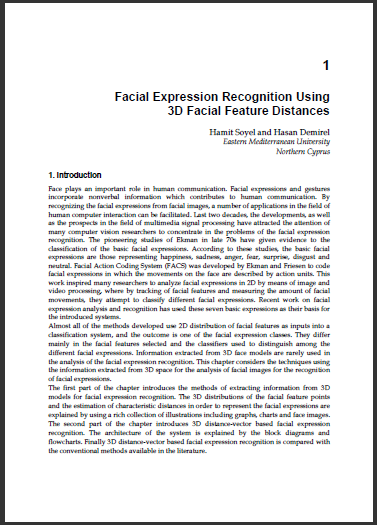
\includegraphics[width=0.5\textwidth]{./chapters/chapter08}
\end{figure}
\lipsum[1]



%%%%%%%%%%%%%%%%%%%%%%%%%%%%%%%%%%%%%%%%%%%
%%%%%%  STYLE 09
%%%%%%%%%%%%%%%%%%%%%%%%%%%%%%%%%%%%%%%%%%%
\clearpage

\cxset{
 name={},
 numbering=arabic,
 number font-size=\LARGE,
 number font-family=\rmfamily,
 number font-weight=\bfseries,
 number before=,
 number dot=.,
 number after=\hspace{1em},
 number position=rightname,
 chapter font-family=\sffamily,
 chapter font-weight=\normalfont,
 chapter font-size=\Large,
 chapter before={\vspace*{20pt}\par\hfill},
 chapter after={},
 chapter color={black!90},
 number color=\color{purple},
 title beforeskip={},
 title afterskip={\vspace*{50pt}\par},
 title before={},
 title after={},
 title font-family=\sffamily,
 title font-color=\color{purple},
 title font-weight=\bfseries,
 title font-size=\LARGE}
\chapter{Introduction 09}
\lipsum[1]

\medskip
\begin{figure}[ht]
\centering

\includegraphics[width=0.8\textwidth]{./chapters/chapter09}
\end{figure}

\textit{In preparation. Patience!}

%%%%%%%%%%%%%%%%%%%%%%%%%%%%%%%%%%%%%%%%%%%
%%%%%%  STYLE 10
%%%%%%%%%%%%%%%%%%%%%%%%%%%%%%%%%%%%%%%%%%%

\cxset{
 name=CHAPTER,
 numbering=WORDS,
 number font-size=\huge,
 number font-family=\sffamily,
 number font-weight=\bfseries,
 number before=,
 number dot=,
 number after=\hspace{1em},
 number position=rightname,
 chapter font-family=\sffamily,
 chapter font-weight=\bfseries,
 chapter font-size=\huge,
 chapter before={\vspace*{0.4\textheight}\hfill},
 chapter after={\hfill\hfill\vskip0pt\thinrule\par},
 chapter color={black!90},
 number color=\color{black!90},
 title beforeskip={\vspace*{30pt}},
 title afterskip={\vspace*{30pt}\par},
 title before={\hfill},
 title after={\hfill\hfill},
 title font-family=\sffamily,
 title font-color=\color{black!90},
 title font-weight=\bfseries,
 title font-size=\huge,
 section font-size=\LARGE,
 section font-weight=\normalfont,
 section font-family=\sffamily,
 section align=,
 section numbering=none,
 section indent=-1em,
 section align=\centering,
 section beforeskip=20pt,
 section afterskip=10pt,
 section spaceout=soul,
 section font-shape=,
}

 %set the sectioning commands
 

\renewsection

\chapter{INTRODUCTION TO STYLE TEN}

\section{Basic Description:}
This chapter style has the unique characteristic that the chapter number is spelled out, rather than being in arabic numerals. The setting for this is the option \lstinline{numeric=WORDS}. Use either a capital for uppercase or \lstinline{numeric=words} for lowercase number labels.

\medskip
\begin{figure}[ht]
\centering
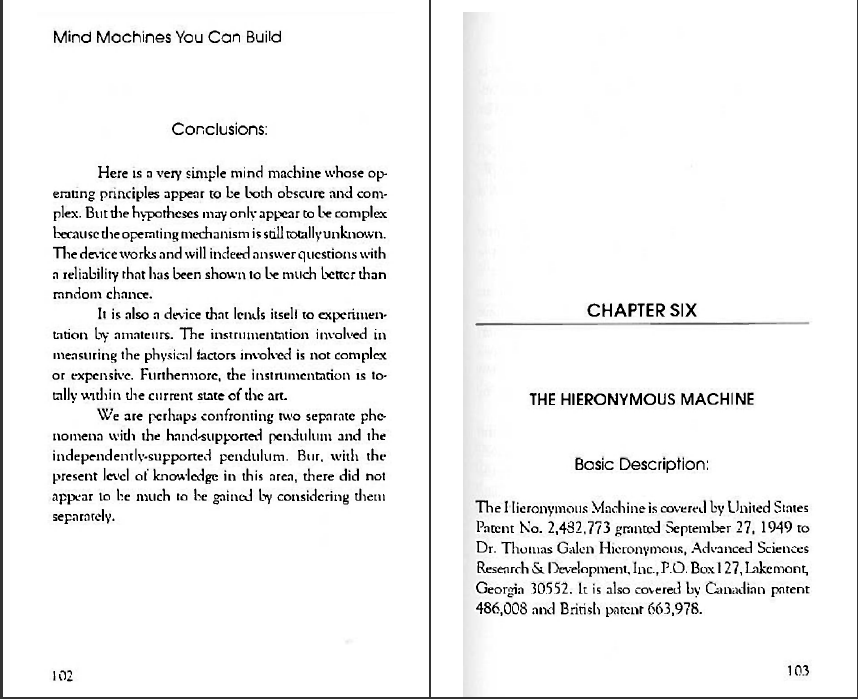
\includegraphics[width=0.6\textwidth]{./chapters/chapter10}
\end{figure}

\lipsum[1]


%%%%%%%%%%%%%%%%%%%%%%%%%%%%%%%%%%%%%%%%%%%
%%%%%%  STYLE 11
%%%%%%%%%%%%%%%%%%%%%%%%%%%%%%%%%%%%%%%%%%%

\cxset{style11/.style={
 name={Chapter},
 numbering=arabic,
 number font-size=\LARGE,
 number font-family=\rmfamily,
 number font-weight=\bfseries,
 number before=,
 number dot=,
 number after=,
 number position=rightname,
 chapter font-family=\rmfamily,
 chapter font-weight=\bfseries,
 chapter font-size=\LARGE,
 chapter before={\vspace*{20pt}\par\hfill},
 chapter after={\hfill\hfill\par\vspace{10pt}},
 chapter color={black!90},
 number color=\color{black!90},
 title beforeskip={},
 title afterskip={\vspace*{20pt}\par},
 title before={\hfill},
 title after={\hfill\hfill\par},
 title font-family=\rmfamily,
 title font-color=\color{black!90},
 title font-weight=\bfseries,
 title font-size=\LARGE}}

\cxset{style11}
\chapter{Introduction to Style Eleven}
\lipsum[2]

\medskip
\begin{figure}[ht]
\centering
\fbox{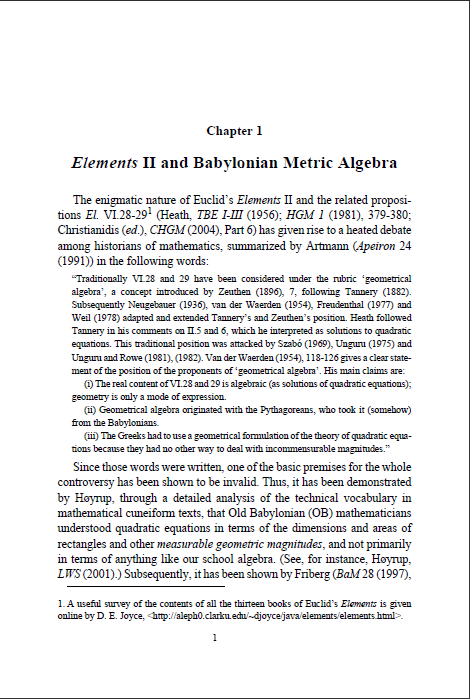
\includegraphics[width=0.65\textwidth]{./chapters/chapter11}}
\end{figure}
\lipsum[1]

%%%%%%%%%%%%%%%%%%%%%%%%%%%%%%%%%%%%%%%%%%%
%%%%%%  STYLE 12
%%%%%%%%%%%%%%%%%%%%%%%%%%%%%%%%%%%%%%%%%%%
\cxset{style12/.style={
 name={},
 numbering=arabic,
 number font-size=\HUGE,
 number font-family=\rmfamily,
 number font-weight=\bfseries,
 number before=,
 number dot=,
 number color=\color{gray},
 number after=\par,
 number position=rightname,
 chapter font-family=\sffamily,
 chapter font-weight=\normalfont,
 chapter font-size=\Huge,
 chapter before={\raggedright\par},
 chapter after={},
 chapter color={black!90},
 title beforeskip={\vspace*{30pt}},
 title afterskip={\vspace*{50pt}\par},
 title before={},
 title after={\par\vspace{30pt}\rule{\textwidth}{4pt}},
 title font-family=\sffamily,
 title font-color=\color{purple},
 title font-weight=\bfseries,
 title font-size=\HUGE,
 title spaceout=none,
}}


\cxset{style12}
\chapter{Introduction to \\ Style Twelve}

This is a variation of Style 7, with only the lettering and the rule are thicker. In my opinion it looks better with a bit of color, so I have used a purple color with a gray.

\medskip
\begin{figure}[ht]
\centering
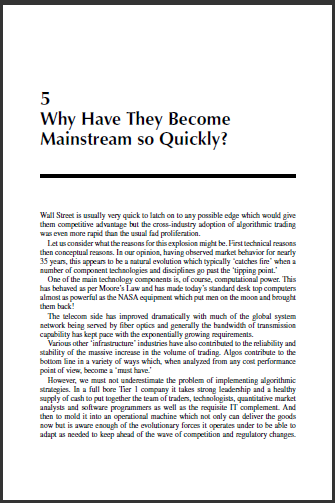
\includegraphics[width=0.35\textwidth]{./chapters/chapter12}
\end{figure}
\lipsum[1]

%%%%%%%%%%%%%%%%%%%%%%%%%%%%%%%%%%%%%%%%%%%
%%%%%%  STYLE 13
%%%%%%%%%%%%%%%%%%%%%%%%%%%%%%%%%%%%%%%%%%%

\cxset{style13/.style={
 name={Chapter},
 numbering=arabic,
 number font-size=\HUGE,
 number font-family=\sffamily,
 number font-weight=\bfseries,
 number color=\color{gray!50},
 number before=\par\vspace*{5pt}\hfill\hfill,
 number dot=,
 number after={\hspace*{7pt}\par},
 number position=rightname,
 chapter font-family=\sffamily,
 chapter font-weight=\normalfont,
 chapter font-size=\LARGE,
 chapter before={\thinrule\vspace*{20pt}\par\hfill\hfill},
 chapter after={\vskip0pt\par},
 chapter color={black!50},
 title beforeskip={\vspace*{10pt}},
 title afterskip={\vspace*{50pt}\par},
 title before={\hfill\hfill\raggedleft},
 title after={},
 title font-family=\sffamily,
 title font-color=\color{purple},
 title font-weight=\bfseries,
 title font-size=\huge,
 section indent=-1em,
 section align=\raggedright,
 section numbering=arabic,
 section indent=0pt,
 section beforeskip=0pt,
 section afterskip=\baselineskip,
 subsection align=\raggedright,
 subsection font-family=\sffamily,
 subsection font-weight=\bfseries,
 subsection font-size=\large,
 subsection font-shape=\itshape,
 subparagraph number after=\space,
}
}

\def\setstyle#1{\cxset{style#1}%
 \renewsection\renewsubsection\renewsubsubsection%
 \renewparagraph\renewsubparagraph}

\setstyle{13}


\chapter{Introduction to Chapter\\ Style Thirteen}

\section{A Brief History of Biomedical\\ Fluid Mechanics}
\lipsum[1]
\medskip
\begin{figure}[ht]
\centering
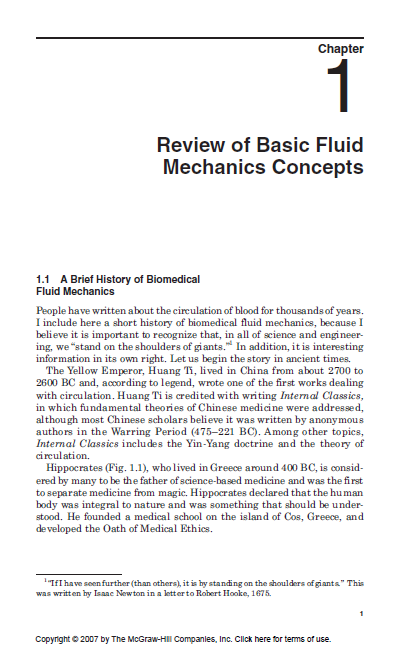
\includegraphics[width=0.45\textwidth]{./chapters/chapter14}
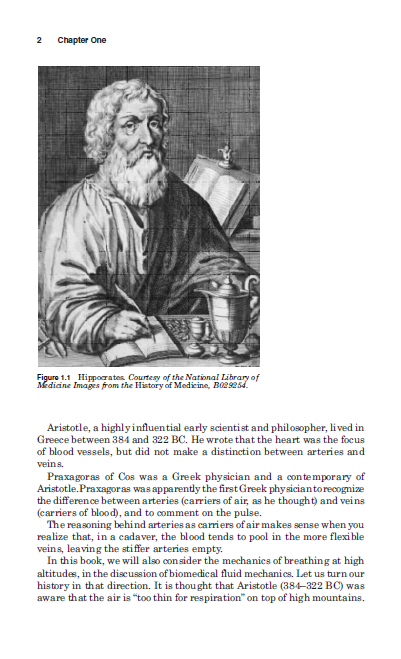
\includegraphics[width=0.45\textwidth]{./chapters/chapter14a}
\end{figure}
\lipsum[2]



%%%%%%%%%%%%%%%%%%%%%%%%%%%%%%%%%%%%%%%%%%%
%%%%%%  STYLE 14
%%%%%%%%%%%%%%%%%%%%%%%%%%%%%%%%%%%%%%%%%%%
\clearpage

\cxset{
 name={},
 numbering=arabic,
 number font-size=\LARGE,
 number font-family=\rmfamily,
 number font-weight=\bfseries,
 number before=,
 number dot=.,
 number after=\hspace{1em},
 number position=rightname,
 chapter font-family=\sffamily,
 chapter font-weight=\normalfont,
 chapter font-size=\Large,
 chapter before={\vspace*{20pt}\par\hfill},
 chapter after={},
 chapter color={black!90},
 number color=\color{purple},
 title beforeskip={},
 title afterskip={\vspace*{50pt}\par},
 title before={},
 title after={},
 title font-family=\sffamily,
 title font-color=\color{purple},
 title font-weight=\bfseries,
 title font-size=\LARGE}
\chapter{Introduction 14}
\lipsum[1]
\medskip
\begin{figure}[ht]
\centering
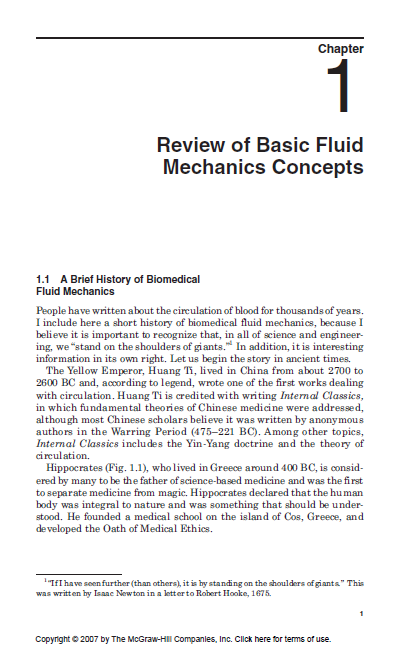
\includegraphics[width=0.65\textwidth]{./chapters/chapter14}
\end{figure}
\lipsum[2]

%%%%%%%%%%%%%%%%%%%%%%%%%%%%%%%%%%%%%%%%%%%
%%%%%%  STYLE 15
%%%%%%%%%%%%%%%%%%%%%%%%%%%%%%%%%%%%%%%%%%%

\cxset{
 name={},
 numbering=arabic,
 number font-size=\LARGE,
 number font-family=\rmfamily,
 number font-weight=\bfseries,
 number before=,
 number dot=.,
 number after=\hspace{1em},
 number position=rightname,
 chapter font-family=\sffamily,
 chapter font-weight=\normalfont,
 chapter font-size=\Large,
 chapter before={\vspace*{20pt}\par\hfill},
 chapter after={},
 chapter color={black!90},
 number color=\color{purple},
 title beforeskip={},
 title afterskip={\vspace*{50pt}\par},
 title before={},
 title after={},
 title font-family=\sffamily,
 title font-color=\color{purple},
 title font-weight=\bfseries,
 title font-size=\LARGE}
\chapter{Introduction 15}
\lipsum[1]
\medskip
\begin{figure}[ht]
\centering
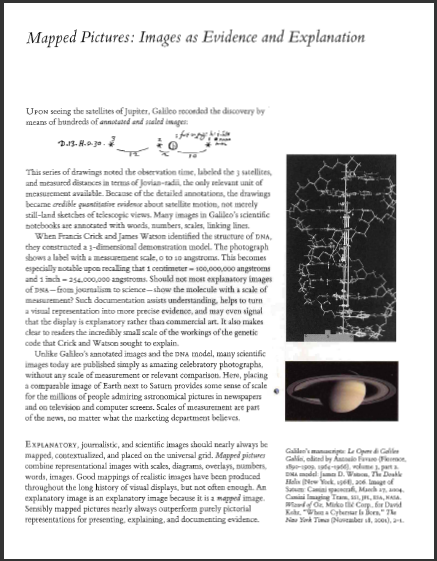
\includegraphics[width=0.65\textwidth]{./chapters/chapter15}
\end{figure}
\lipsum[2]

%%%%%%%%%%%%%%%%%%%%%%%%%%%%%%%%%%%%%%%%%%%
%%%%%%  STYLE 16
%%%%%%%%%%%%%%%%%%%%%%%%%%%%%%%%%%%%%%%%%%%
\cxset{
 name={},
 numbering=arabic,
 number font-size=\LARGE,
 number font-family=\rmfamily,
 number font-weight=\bfseries,
 number before=,
 number dot=.,
 number after=\hspace{1em},
 number position=rightname,
 chapter font-family=\sffamily,
 chapter font-weight=\normalfont,
 chapter font-size=\Large,
 chapter before={\vspace*{20pt}\par\hfill},
 chapter after={},
 chapter color={black!90},
 number color=\color{purple},
 title beforeskip={},
 title afterskip={\vspace*{50pt}\par},
 title before={},
 title after={},
 title font-family=\sffamily,
 title font-color=\color{purple},
 title font-weight=\bfseries,
 title font-size=\LARGE}
\chapter{Introduction 16}
\lipsum[1]
\medskip
\begin{figure}[ht]
\centering
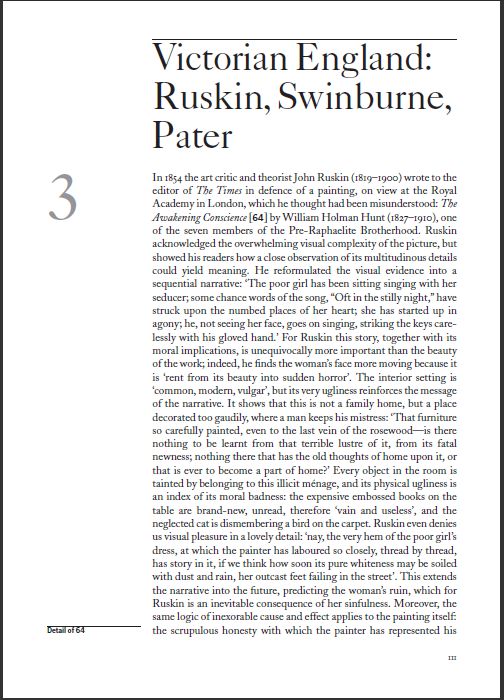
\includegraphics[width=0.65\textwidth]{./chapters/chapter16}
\end{figure}
\lipsum[2]

%%%%%%%%%%%%%%%%%%%%%%%%%%%%%%%%%%%%%%%%%%%
%%%%%%  STYLE 17
%%%%%%%%%%%%%%%%%%%%%%%%%%%%%%%%%%%%%%%%%%%

\cxset{style17/.style={
 name={},
 numbering=arabic,
 number font-size=\LARGE,
 number font-family=\sffamily,
 number font-weight=\bfseries,
 number before=,
 number dot=.,
 number after=\thinspace,
 number position=rightname,
 chapter font-family=\sffamily,
 chapter font-weight=\bfseries,
 chapter font-size=\LARGE,
 chapter before={\vspace*{20pt}\par\hfill},
 chapter after={},
 chapter color={black!90},
 title beforeskip={},
 title afterskip={\vspace*{70pt}\par},
 title before={},
 title after={},
 title font-family=\sffamily,
 title font-color=\color{purple},
 title font-weight=\bfseries,
 title font-size=\LARGE}}
\cxset{style17}
\chapter{Introduction to Style Seventeen}

\lipsum[1]
\medskip
\begin{figure}[ht]
\centering
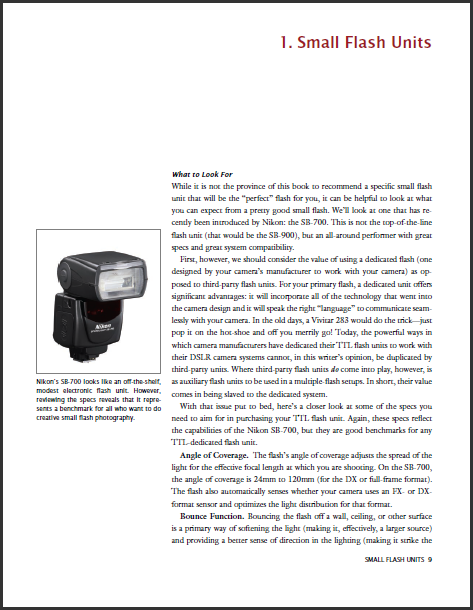
\includegraphics[width=0.5\textwidth]{./chapters/chapter17}
\end{figure}
\lipsum[2-4]

%%%%%%%%%%%%%%%%%%%%%%%%%%%%%%%%%%%%%%%%%%%
%%%%%%  STYLE 18
%%%%%%%%%%%%%%%%%%%%%%%%%%%%%%%%%%%%%%%%%%%

\cxset{
 name={},
 numbering=arabic,
 number font-size=\LARGE,
 number font-family=\rmfamily,
 number font-weight=\bfseries,
 number before=\par\hangindent2em\hangafter1,
 number after=\hspace{1em},
 number position=rightname,
 chapter font-family=\sffamily,
 chapter font-weight=\normalfont,
 chapter font-size=\Large,
 chapter before={\vspace*{20pt}},
 chapter after={},
 chapter color={black!90},
 number color=\color{black!90},
 title beforeskip={},
 title afterskip={\vspace*{50pt}\par},
 title before={},
 title after={},
 title font-family=\sffamily,
 title font-color=\color{black},
 title font-weight=\bfseries,
 title font-size=\LARGE}
\chapter{Introduction to chapter\\ style eighteen}

\parindent0pt
I tend to favour this design for books that have a lot of pictures. It brings the design into the margins and leaves plentiful white space in the margins. From a programming point of view the chapter is the opposite of openany. It has to open on an odd number.
\medskip
\begin{figure}[ht]
\centering
\includegraphics[width=0.65\textwidth]{./chapters/chapter18}
\end{figure}

%%%%%%%%%%%%%%%%%%%%%%%%%%%%%%%%%%%%%%%%%%%
%%%%%%  STYLE 19
%%%%%%%%%%%%%%%%%%%%%%%%%%%%%%%%%%%%%%%%%%%


\cxset{
 name={},
 numbering=arabic,
 number font-size=\LARGE,
 number font-family=\rmfamily,
 number font-weight=\bfseries,
 number before=\par\hangindent2em\hangafter1,
 number after=\hspace{1em},
 number position=rightname,
 chapter font-family=\sffamily,
 chapter font-weight=\normalfont,
 chapter font-size=\Large,
 chapter before={\vspace*{20pt}},
 chapter after={},
 chapter color={black!90},
 number color=\color{black!90},
 title beforeskip={},
 title afterskip={\vspace*{50pt}\par},
 title before={},
 title after={},
 title font-family=\sffamily,
 title font-color=\color{black},
 title font-weight=\bfseries,
 title font-size=\LARGE}
\chapter{Introduction to chapter\\ style nineteen}
\lipsum[1]

\medskip
\begin{figure}[ht]
\centering
\includegraphics[width=0.65\textwidth]{./chapters/chapter19}
\end{figure}

\lipsum[1]

%%%%%%%%%%%%%%%%%%%%%%%%%%%%%%%%%%%%%%%%%%%
%%%%%%  STYLE 21
%%%%%%%%%%%%%%%%%%%%%%%%%%%%%%%%%%%%%%%%%%%

\cxset{
 name={},
 numbering=none,
 number font-size=\Large,
 number font-family=\rmfamily,
 number font-weight=\bfseries,
 number before={},
 number after={},
 number position=rightname,
 chapter font-family=\sffamily,
 chapter font-weight=\normalfont,
 chapter font-size=\Large,
 chapter before={\vspace*{0.3\textheight}},
 chapter after={\par},
 chapter color={black!90},
 number color=\color{black!90},
 title beforeskip={},
 title afterskip={\par\rule{\textwidth}{3.5pt}\vspace{20pt}},
 title before={},
 title after={},
 title font-family=\sffamily,
 title font-color=\color{black},
 title font-weight=\bfseries,
 title font-size=\Huge}
\chapter{INTRODUCTION TO STYLE 21}

\lipsum[1]
\medskip
\begin{figure}[ht]
\centering
\fbox{\includegraphics[width=0.65\textwidth]{./chapters/chapter21}}
\end{figure}
\lipsum[1]

%%%%%%%%%%%%%%%%%%%%%%%%%%%%%%%%%%%%%%%%%%%
%%%%%%  STYLE 22
%%%%%%%%%%%%%%%%%%%%%%%%%%%%%%%%%%%%%%%%%%%

\newgeometry{left=2.5in}
\cxset{style22/.style={
 name={},
 numbering=none,
 number font-size=\Large,
 number font-family=\rmfamily,
 number font-weight=\bfseries,
 number before={},
 number after={},
 number position=rightname,
 chapter font-family=\sffamily,
 chapter font-weight=\normalfont,
 chapter font-size=\Large,
 chapter before={\vspace*{-80pt}},
 chapter after={\par},
 chapter color={black!90},
 number color=\color{black!90},
 title beforeskip={\hfill},
 title afterskip={\vspace{70pt}},
 title before=\hspace*{-1in},
 title after={},
 title font-family=\sffamily,
 title font-color=\color{black},
 title font-weight=\bfseries,
 title font-size=\huge,
 section numbering=none,
 section font-weight=\bfseries,
 section indent=-1em}}

\setstyle{22}

\chapter{INTRODUCTION TO STYLE TWENTY TWO}

\section{INTRODUCTION}

\lettrine{Y}{annis}. \lipsum[2]

\medskip
\begin{figure}[ht]
\centering
\fbox{\includegraphics[width=0.5\textwidth]{./chapters/chapter22}}
\end{figure}

\lipsum[1-2]

\setcounter{secnumdepth}{6}
%%%%%%%%%%%%%%%%%%%%%%%%%%%%%%%%%%%%%%%%%%%
%%%%%%  STYLE 23
%%%%%%%%%%%%%%%%%%%%%%%%%%%%%%%%%%%%%%%%%%%
\newgeometry{left=4cm,right=4cm,bottom=2cm}

\cxset{style23/.style={
 name={Chapter},
 numbering=arabic,
 number font-size=\Large,
 number font-family=\rmfamily,
 number font-weight=\bfseries,
 number before={},
 number after={},
 number dot=,
 number position=rightname,
 chapter font-family=\sffamily,
 chapter font-weight=\normalfont,
 chapter font-size=\Large,
 chapter before={\hspace*{-50pt}\rule{\dimexpr\textwidth+50pt\relax}{0.4pt}\par\hspace*{-51pt}},
 chapter after={\par},
 chapter color={black!90},
 number color=\color{gray},
 title beforeskip={},
 title afterskip={\vspace{30pt}},
 title before=\hspace*{-50pt},
 title after={\par\vspace*{-10pt}\hspace*{-50pt}\rule{\dimexpr\textwidth+50pt}{0.4pt}\par},
 title font-family=\rmfamily,
 title font-color=\color{black!80},
 title font-weight=\bfseries,
 title font-size=\LARGE,
 section font-family=\rmfamily,
 section font-shape=\itshape,
 section font-weight=\bfseries,
 section numbering=arabic,
 section indent=-49pt,
 section beforeskip=\baselineskip,
 section afterskip=\baselineskip,
% subsection commands
 subsection font-shape=\upshape,
 subsection beforeskip=\baselineskip,
 subsection afterskip=10pt,
 subsection indent=-49pt,
 subsection numbering=arabic,
% subsection commands
 subsubsection font-family=\rmfamily,
 subsubsection font-shape=\itshape,
 subsubsection font-weight=\bfseries,
 subsubsection font-shape=\itshape,
 subsubsection font-size=\large,
 subsubsection align=,
 subsubsection beforeskip=10pt,
 subsubsection afterskip=\baselineskip,
 subsubsection indent=-49pt,
 subsubsection numbering=numeric,
% paragraphs
 paragraph font-family=\rmfamily,
 paragraph font-shape=\itshape,
 paragraph font-weight=\normalfont,
 paragraph font-shape=\itshape,
 paragraph font-size=\large,
 paragraph align=,
 paragraph beforeskip=10pt,
 paragraph afterskip=0pt,
 paragraph indent=-49pt,
 paragraph numbering=numeric,
% subparagraphs
 subparagraph font-family=\rmfamily,
 subparagraph font-shape=\itshape,
 subparagraph font-weight=\normalfont,
 subparagraph font-shape=\itshape,
 subparagraph font-size=\large,
 subparagraph align=,
 subparagraph beforeskip=10pt,
 subparagraph afterskip=0pt,
 subparagraph indent=-49pt,
 subparagraph numbering=arabic,
 subparagraph number after=\thinspace,
 header style=empty,
 pagestyle=headings,
}}

\cxset{headings style58}
\setstyle{23}
\chapter{Introduction to style twenty three}

\section{Introduction}

This style requires that the chapter settings as well as the
section headings are set in the margins, leaving the text after the sectioning commands to be indented. We achieve this by using negative skips. 
\medskip
\begin{figure}[ht]
\centering
\fbox{\includegraphics[width=0.45\textwidth]{./chapters/chapter23}
\includegraphics[width=0.45\textwidth]{./chapters/chapter23a}}
\end{figure}

\subsection{Subsections}
The same style is applied to the subsectioning commands up to the subsubsection which is not numbered but just uses an italic font. The subsubsection is also indented into the margin. Since the book is about construction claims it follows a style found in legal and construction documents, where all paragraphs are indented with respect to the section headings.
\lipsum[1-2]
\section{Even pages}
\lipsum[2]
\subsection{Setting different margins}
\lipsum[1]
\subsubsection{Setting Subsubsections}
\lipsum[1]
\paragraph{Paragraph level. } \lipsum*[3]\par

\lipsum[1]
\subparagraph{sub-paragraph level. } \lipsum*[3]\par

\restoregeometry
%%%%%%%%%%%%%%%%%%%%%%%%%%%%%%%%%%%%%%%%%%%
%%%%%%  STYLE 24
%%%%%%%%%%%%%%%%%%%%%%%%%%%%%%%%%%%%%%%%%%%
\clearpage
\cxset{
 name=Chapter,
 numbering=arabic,
 number font-size=\Large,
 number font-family=\sffamily,
 number font-weight=\normalfont,
 number before={},
 number after={\space},
 number position=rightname,
 chapter font-family=\sffamily,
 chapter font-weight=\normalfont,
 chapter font-size=\Large,
 number after={},
 number dot=,
 chapter before={},
 chapter after={\par\thinrule\vskip12pt},
 chapter color={black!90},
 number color=\color{black!90},
 title beforeskip={},
 title afterskip={\vspace{30pt}},
 title before=,
 title after={\par},
 title font-family=\sffamily,
 title font-color=\color{black!80},
 title font-weight=\bfseries,
 title font-size=\LARGE,
 title afterskip=\par\vspace*{3cm}\thinrule\par\bigskip\bigskip}
\chapter{Introduction to style twenty four}

\def\objectives@{
\begin{tcolorbox}[width=\linewidth,boxsep=10pt,right=10pt]
\textbf{Learning Objectives}}
\def\stopobjectives@{\end{tcolorbox}}
\newenvironment{objectives}{\bigskip\objectives@}{\stopobjectives@\bigskip}

\begin{objectives}
\par
\lipsum[1]
\bigskip\bigskip
\end{objectives}

This design is ideal for scholarly books or notes. It has a nice clean design with a shaded block for the learning objectives.
\medskip
\begin{figure}[ht]
\centering
\fbox{\includegraphics[width=0.6\textwidth]{./chapters/chapter24}}
\end{figure}
\lipsum[2-3]


%%%%%%%%%%%%%%%%%%%%%%%%%%%%%%%%%%%%%%%%%%%
%%%%%%  STYLE 25
%%%%%%%%%%%%%%%%%%%%%%%%%%%%%%%%%%%%%%%%%%%

\cxset{author/.store in=\author@cx}

\cxset{style25/.style={
 name={CHAPTER},
 numbering=arabic,
 number font-size=\huge,
 number font-family=\sffamily,
 number font-weight=\normalfont,
 number before={},
 number position=rightname,
 chapter font-family=\sffamily,
 chapter font-weight=\normalfont,
 chapter font-size=\huge,
 number after={},
 chapter before={\thinrule\par\vspace{3pt}\hfill},
 chapter after={\hfill\hfill\par\vspace{-10pt}\thinrule\par\leavevmode},
 chapter color={black!90},
 number color=\color{black!90},
 title beforeskip={\centering},
 title afterskip={\vspace{20pt}\author@cx},
 title before=\leavevmode,
 title after={\par\vspace{-20pt}\thinrule\par},
 title font-family=\sffamily,
 title font-color=\color{black!80},
 title font-weight=\bfseries,
 title font-size=\huge}}

\cxset{author=\centering\bfseries\upshape\large Yiannis Lazarides and Athena Lazarides\par\vspace{30pt}}

\setstyle{25}
\chapter{INTRODUCTION TO STYLE 25}

The interesting part of this style is that it uses roman numerals to display the counter that is in a different font than that used for the chapter name.
\medskip
\begin{figure}[ht]
\centering
\fbox{\includegraphics[width=0.5\textwidth]{chapter25}}
\end{figure}
\lipsum[1-2]

%\end{document}
%%%%%%%%%%%%%%%%%%%%%%%%%%%%%%%%%%%%%%%%%%%
%%%%%%  STYLE 26
%%%%%%%%%%%%%%%%%%%%%%%%%%%%%%%%%%%%%%%%%%%

\cxset{
 name={},
 numbering=arabic,
 number font-size=\huge,
 number font-family=\sffamily,
 number font-weight=\bfseries,
 number before={},
 number position=leftname,
 chapter font-family=\sffamily,
 chapter font-weight=\normalfont,
 chapter font-size=\small,
 number after={},
 chapter before={},
 chapter after={\par\vskip12pt},
 chapter color={black!90},
 number color=\color{black!90},
 title beforeskip={},
 title afterskip={\vspace{30pt}},
 title before=,
 title after={\par},
 title font-family=\sffamily,
 title font-color=\color{black!80},
 title font-weight=\bfseries,
 title font-size=\LARGE}
\chapter{Introduction to style twenty five Dr. Yiannis Lazarides and Athena Lazarides}

The interesting part of this style is that it uses roman numerals to display the counter that is in a different font than that used for the chapter name.
\medskip
\begin{figure}[ht]
\centering
\fbox{\includegraphics[width=0.6\textwidth]{./chapters/chapter26}}
\end{figure}
\lipsum[2-3]


\newgeometry{top=2cm,bottom=2cm}
%%%%%%%%%%%%%%%%%%%%%%%%%%%%%%%%%%%%%%%%%%%
%%%%%%  STYLE 27
%%%%%%%%%%%%%%%%%%%%%%%%%%%%%%%%%%%%%%%%%%%

\cxset{
 name={},
 numbering=arabic,
 number font-size=\HUGE,
 number font-family=\sffamily,
 number font-weight=\bfseries,
 number before={},
 number dot=,
 number position=leftname,
 chapter font-family=\sffamily,
 chapter font-weight=\normalfont,
 chapter font-size=\small,
 number after={},
 chapter before={\vspace*{50pt}},
 chapter after={\par\vskip12pt},
 chapter color={black!90},
 number color=\color{black!90},
 title beforeskip={},
 title afterskip={\vspace{30pt}},
 title before=,
 title after={\par},
 title font-family=\sffamily,
 title font-color=\color{black!80},
 title font-weight=\bfseries,
 title font-size=\huge}
\chapter{Introduction to style twenty seven Dr. Yiannis Lazarides and Athena Lazarides}
\lipsum[3]

\medskip
\begin{figure}[ht]
\centering
\fbox{\includegraphics[width=0.5\textwidth]{./chapters/chapter27}}
\end{figure}
\lipsum[2-3]


%%%%%%%%%%%%%%%%%%%%%%%%%%%%%%%%%%%%%%%%%%%
%%%%%%  STYLE 28
%%%%%%%%%%%%%%%%%%%%%%%%%%%%%%%%%%%%%%%%%%%

\cxset{
 name={},
 numbering=arabic,
 number font-size=\HUGE,
 number font-family=\sffamily,
 number font-weight=\bfseries,
 number before={},
 number position=leftname,
 chapter font-family=\sffamily,
 chapter font-weight=\normalfont,
 chapter font-size=\small,
 number after={},
 chapter before={},
 chapter after={\hspace*{20pt}},
 chapter color={black!90},
 number color=\color{black!90},
 title beforeskip={},
 title afterskip={\vspace{70pt}},
 title before=,
 title after={\par},
 title font-family=\itshape,
 title font-color=\color{black!80},
 title font-weight=\itshape,
 title font-size=\LARGE}
\chapter{Introduction to Style Twenty Eight}

The interesting part of this style is that it uses roman numerals to display the counter that is in a different font than that used for the chapter name.
\medskip
\begin{figure}[ht]
\centering
\includegraphics[width=0.6\textwidth]{./chapters/chapter28}
\end{figure}
\lipsum[2]

%%%%%%%%%%%%%%%%%%%%%%%%%%%%%%%%%%%%%%%%%%%
%%%%%%  STYLE 29
%%%%%%%%%%%%%%%%%%%%%%%%%%%%%%%%%%%%%%%%%%%
 \cxset{
 name={},
 numbering=arabic,
 number font-size=\HUGE,
 number font-family=\sffamily,
 number font-weight=\bfseries,
 number before={},
 number position=leftname,
 chapter font-family=\sffamily,
 chapter font-weight=\normalfont,
 chapter font-size=\small,
 number after={},
 chapter before={},
 chapter after={\hspace*{20pt}},
 chapter color={black!90},
 number color=\color{black!90},
 title beforeskip={},
 title afterskip={\vspace{70pt}},
 title before=,
 title after={\par},
 title font-family=\itshape,
 title font-color=\color{black!80},
 title font-weight=\itshape,
 title font-size=\LARGE}
\chapter{Introduction to Style Twenty Nine}

The interesting part of this style is that it uses roman numerals to display the counter that is in a different font than that used for the chapter name.
\medskip
\begin{figure}[ht]
\centering
\includegraphics[width=0.6\textwidth]{./chapters/chapter29}
\end{figure}
\lipsum[3]

%%%%%%%%%%%%%%%%%%%%%%%%%%%%%%%%%%%%%%%%%%%
%%%%%%  STYLE 30
%%%%%%%%%%%%%%%%%%%%%%%%%%%%%%%%%%%%%%%%%%%

\cxset{style30/.style={
 name={},
 numbering=arabic,
 number font-size=\HUGE,
 number font-family=\sffamily,
 number font-weight=\bfseries,
 number before={\rule{\textwidth}{5pt}\par\vspace*{12pt}\hspace*{20pt}\minipage{1cm}\vspace*{8pt}},
 number after=\endminipage\hspace{1em},
 number position=leftname,
 chapter font-family=\sffamily,
 chapter font-weight=\normalfont,
 chapter font-size=\small,
 chapter before={},
 chapter after={\hspace*{20pt}},
 chapter color={black!90},
 number color=\color{black!90},
 title beforeskip={},
 title afterskip={\vspace{30pt}},
 title before=\minipage[t]{10cm},
 title after={\endminipage\par},
 title font-family=\sffamily,
 title font-color=\color{black!80},
 title font-weight=\normalfont\sffamily,
 title font-size=\huge}}

\cxset{style30}
\chapter{Introduction to Style Thirty\\ with a somehow long title \\to illustrate the example}

Since we do not know how long a chapter title can end up, it is best to
typeset this using two minipages or parboxes. The number is pushed down slightly although it can look as good with both the number and the text fully aligned on top.
\medskip
\begin{figure}[ht]
\centering
\includegraphics[width=0.6\textwidth]{./chapters/chapter30}
\end{figure}



%%%%%%%%%%%%%%%%%%%%%%%%%%%%%%%%%%%%%%%%%%%
%%%%%%  STYLE 31
%%%%%%%%%%%%%%%%%%%%%%%%%%%%%%%%%%%%%%%%%%%

\cxset{style31/.style={
 name={},
 numbering=arabic,
 number font-size=\HUGE,
 number font-family=\sffamily,
 number font-weight=\bfseries,
 number before=,
 number after={},
 number position=leftname,
 chapter font-family=\sffamily,
 chapter font-weight=\normalfont,
 chapter font-size=\small,
 chapter before={},
 chapter after={\par{\color{gray}\rule{3cm}{5pt}\rule[3.5pt]{\dimexpr\textwidth-3cm\relax}{0.4pt}}\par},
 chapter color={gray},
 number color=\color{gray},
 title beforeskip={},
 title afterskip={\vspace{30pt}},
 title before=,
 title after={\par{\color{gray}\rule[6pt]{3cm}{0.4pt}}\par},
 title font-family=\itshape,
 title font-color=\color{black},
 title font-weight=\itshape,
 title font-size=\LARGE}}

\cxset{style31}
\chapter{The Evolution of Organizations\\ and the Environment}

This is an unusual design by all counts. I did soften the rules a bit to make them a bit less conspicuous. 
\medskip
\begin{figure}[ht]
\centering
\includegraphics[width=0.6\textwidth]{./chapters/chapter31}
\end{figure}

\lipsum[1-2]

%%%%%%%%%%%%%%%%%%%%%%%%%%%%%%%%%%%%%%%%%%%
%%%%%%  STYLE 32
%%%%%%%%%%%%%%%%%%%%%%%%%%%%%%%%%%%%%%%%%%%

\cxset{
 name={},
 numbering=arabic,
 number font-size=\HUGE,
 number font-family=\sffamily,
 number font-weight=\bfseries,
 number before={\hspace*{-20pt}},
 number position=leftname,
 chapter font-family=\sffamily,
 chapter font-weight=\normalfont,
 chapter font-size=\small,
 number after={},
 chapter before={\vspace*{50pt}\par\hspace*{-50pt}},
 chapter after={\hspace*{20pt}},
 chapter color={black!90},
 number color=\color{black!90},
 title beforeskip={},
 title afterskip={\vspace{50pt}},
 title before=,
 title after={\par},
 title font-family=\itshape,
 title font-color=\color{black!80},
 title font-weight=\itshape,
 title font-size=\LARGE}
\chapter{Introduction to Style Thirty Two}

This style has a modern look to it. Its main characteristic is the large chapter number and the fact that it is drawn into the margin. A common style for computer books.
\medskip
\begin{figure}[ht]
\centering
\includegraphics[width=0.6\textwidth]{./chapters/chapter32}
\end{figure}
The example is from Python NLP book.

%%%%%%%%%%%%%%%%%%%%%%%%%%%%%%%%%%%%%%%%%%%
%%%%%%  STYLE 33
%%%%%%%%%%%%%%%%%%%%%%%%%%%%%%%%%%%%%%%%%%%

\cxset{
 name=CHAPTER,
 numbering=Roman,
 number font-size=\small,
 number font-family=\rmfamily,
 number font-weight=\normalfont,
 number before={},
 number position=rightname,
 chapter font-family=\sffamily,
 chapter font-weight=\normalfont,
 chapter font-size=\small,
 number after={},
 chapter before={},
 chapter after={\par},
 chapter color={black!90},
 number color=\color{black!90},
 title beforeskip={},
 title afterskip={\vspace{50pt}},
 title before=,
 title after={\par},
 title font-family=\normalfont,
 title font-color=\color{black!80},
 title font-weight=\normalfont,
 title font-size=\LARGE}
\chapter{Introduction to Style Thirty Three}

The interesting part of this style is that it uses roman numerals to display the counter that is in a different font than that used for the chapter name.
\medskip
\begin{figure}[ht]
\centering
\includegraphics[width=0.6\textwidth]{./chapters/chapter33}
\end{figure}





%%%%%%%%%%%%%%%%%%%%%%%%%%%%%%%%%%%%%%%%%%%
%%%%%%  STYLE 34
%%%%%%%%%%%%%%%%%%%%%%%%%%%%%%%%%%%%%%%%%%%

\cxset{
 name=CHAPTER,
 numbering=Roman,
 number font-size=\small,
 number font-family=\rmfamily,
 number font-weight=\normalfont,
 number before={},
 number position=rightname,
 chapter font-family=\sffamily,
 chapter font-weight=\normalfont,
 chapter font-size=\small,
 number after={},
 chapter before={},
 chapter after={\par},
 chapter color={black!90},
 number color=\color{black!90},
 title beforeskip={},
 title afterskip={\vspace{50pt}},
 title before=,
 title after={\par},
 title font-family=\normalfont,
 title font-color=\color{black!80},
 title font-weight=\normalfont,
 title font-size=\LARGE}
\section{Introduction to Style Thirty Four}

The interesting part of this style is that it uses roman numerals to display the counter that is in a different font than that used for the chapter name.
\medskip
\begin{figure}[ht]
\centering
\includegraphics[width=0.6\textwidth]{./chapters/chapter34}
\end{figure}


%%%%%%%%%%%%%%%%%%%%%%%%%%%%%%%%%%%%%%%%%%%
%%%%%%  STYLE 35
%%%%%%%%%%%%%%%%%%%%%%%%%%%%%%%%%%%%%%%%%%%

\cxset{%
 name=CHAPTER,
 numbering=Roman,
 number font-size=\small,
 number font-family=\rmfamily,
 number font-weight=\normalfont,
 number before={},
 number position=rightname,
 chapter font-family=\sffamily,
 chapter font-weight=\normalfont,
 chapter font-size=\small,
 number after={},
 chapter before={},
 chapter after={\par},
 chapter color={black!90},
 number color=\color{black!90},
 title beforeskip={},
 title afterskip={\vspace{50pt}},
 title before=,
 title after={\par},
 title font-family=\normalfont,
 title font-color=\color{black!80},
 title font-weight=\normalfont,
 title font-size=\LARGE}
\chapter{Introduction to Style Thirty Five}

The interesting part of this style is that it uses roman numerals to display the counter that is in a different font than that used for the chapter name.
\medskip

\begin{figure}[ht]
\centering
\includegraphics[width=0.6\textwidth]{./chapters/chapter35}
\end{figure}


%%%%%%%%%%%%%%%%%%%%%%%%%%%%%%%%%%%%%%%%%%%
%%%%%%  STYLE 36
%%%%%%%%%%%%%%%%%%%%%%%%%%%%%%%%%%%%%%%%%%%

\cxset{
 name=CHAPTER,
 numbering=Roman,
 number font-size=\small,
 number font-family=\rmfamily,
 number font-weight=\normalfont,
 number before={},
 number position=rightname,
 chapter font-family=\sffamily,
 chapter font-weight=\normalfont,
 chapter font-size=\small,
 number after={},
 chapter before={},
 chapter after={\par},
 chapter color={black!90},
 number color=\color{black!90},
 title beforeskip={},
 title afterskip={\vspace{50pt}},
 title before=,
 title after={\par},
 title font-family=\normalfont,
 title font-color=\color{black!80},
 title font-weight=\normalfont,
 title font-size=\LARGE}
\chapter{Introduction to Style Thirty Six}

The interesting part of this style is that it uses roman numerals to display the counter that is in a different font than that used for the chapter name.
\medskip

\begin{figure}[ht]
\centering
\includegraphics[width=0.6\textwidth]{./chapters/chapter36}
\end{figure}


%%%%%%%%%%%%%%%%%%%%%%%%%%%%%%%%%%%%%%%%%%%
%%%%%%  STYLE 37
%%%%%%%%%%%%%%%%%%%%%%%%%%%%%%%%%%%%%%%%%%%

\cxset{
 name=CHAPTER,
 numbering=Roman,
 number font-size=\small,
 number font-family=\rmfamily,
 number font-weight=\normalfont,
 number before={},
 number position=rightname,
 chapter font-family=\sffamily,
 chapter font-weight=\normalfont,
 chapter font-size=\small,
 number after={},
 chapter before={},
 chapter after={\par},
 chapter color={black!90},
 number color=\color{black!90},
 title beforeskip={},
 title afterskip={\vspace{50pt}},
 title before=,
 title after={\par},
 title font-family=\normalfont,
 title font-color=\color{black!80},
 title font-weight=\normalfont,
 title font-size=\LARGE}
\chapter{Introduction to Style Thirty Seven}

The interesting part of this style is that it uses roman numerals to display the counter that is in a different font than that used for the chapter name.
\medskip

\begin{figure}[ht]
\centering
\includegraphics[width=0.6\textwidth]{./chapters/chapter37}
\end{figure}


%%%%%%%%%%%%%%%%%%%%%%%%%%%%%%%%%%%%%%%%%%%
%%%%%%  STYLE 38
%%%%%%%%%%%%%%%%%%%%%%%%%%%%%%%%%%%%%%%%%%%

\cxset{
 name=CHAPTER,
 numbering=arabic,
 number font-size=\LARGE,
 number font-family=\sffamily,
 number font-weight=\bfseries,
 number before={},
 number position=rightname,
 chapter font-family=\sffamily,
 chapter font-weight=\bfseries,
 number after={},
 chapter before={\rule{\textwidth}{2pt}\par},
 chapter after={\vskip0pt\vspace*{-8pt}\rule{\textwidth}{.4pt}\vskip-7pt},
 chapter color={black!90},
 number color=\color{black!90},
 title beforeskip={},
 title afterskip={\vspace{50pt}},
 title before=,
 title after={\par\vskip-19pt\rule{\textwidth}{0.4pt}\par} ,
 title font-family=\sffamily,
 title font-color=\color{black!80},
 title font-weight=\bfseries,
 title font-size=\LARGE,
 chapter font-size=\LARGE}
\chapter{INTRODUCTION}

This style uses rules to enclose both the chapter name and number as well as the title, which necessarily needs to be rather short.
\medskip

\begin{figure}[ht]
\centering
\includegraphics[width=0.6\textwidth]{./chapters/chapter38}
\end{figure}



%%%%%%%%%%%%%%%%%%%%%%%%%%%%%%%%%%%%%%%%%%%
%%%%%%  STYLE 39
%%%%%%%%%%%%%%%%%%%%%%%%%%%%%%%%%%%%%%%%%%%

\cxset{
 name=CHAPTER,
 numbering=arabic,
 number font-size=\LARGE,
 number font-family=\sffamily,
 number font-weight=\bfseries,
 number before={},
 number position=rightname,
 chapter font-family=\sffamily,
 chapter font-weight=\bfseries,
 number after={},
 chapter before={\rule{\textwidth}{2pt}\par},
 chapter after={\vskip0pt\vspace*{-8pt}\rule{\textwidth}{.4pt}\vskip-7pt},
 chapter color={black!90},
 number color=\color{black!90},
 title beforeskip={},
 title afterskip={\vspace{50pt}},
 title before=,
 title after={\par\vskip-19pt\rule{\textwidth}{0.4pt}\par} ,
 title font-family=\sffamily,
 title font-color=\color{black!80},
 title font-weight=\bfseries,
 title font-size=\LARGE,
 chapter font-size=\LARGE}

\chapter{INTRODUCTION}

This style uses rules to enclose both the chapter name and number as well as the title, which necessarily needs to be rather short.
\medskip

\begin{figure}[ht]
\centering
\includegraphics[width=0.6\textwidth]{./chapters/chapter39}
\end{figure}
In the picture it does not look very attractive, but in the actual book it does. My observation is that the rule clearances are a bit tight and if you use this type of layout it is better to experiment until you get them right.

\begin{tcblisting}{}
\@makechapterhead[
 name=CHAPTER,
 numbering=arabic,
 number font-size=\LARGE,
 number font-family=\sffamily,
 number font-weight=\bfseries,
 number before={},
 number position=rightname,
 chapter font-family=\sffamily,
 chapter font-weight=\bfseries,
 number after={},
 chapter before={\rule{\textwidth}{2pt}\par},
 chapter after={\vskip0pt\vspace*{-8pt}\rule{\textwidth}{.4pt}\vskip-7pt},
 chapter color={black!90},
 number color=\color{black!90},
 title beforeskip={},
 title afterskip={\vspace{50pt}},
 title before=,
 title after={\par\vskip-19pt\rule{\textwidth}{0.4pt}\par} ,
 title font-family=\sffamily,
 title font-color=\color{black!80},
 title font-weight=\bfseries,
 title font-size=\LARGE,
 chapter font-size=\LARGE]{INTRODUCTION}
\end{tcblisting}


%%%%%%%%%%%%%%%%%%%%%%%%%%%%%%%%%%%%%%%%%%%
%%%%%%  STYLE 40
%%%%%%%%%%%%%%%%%%%%%%%%%%%%%%%%%%%%%%%%%%%

\cxset{
 name=,
 numbering=arabic,
 number font-size=\LARGE,
 number font-family=\sffamily,
 number font-weight=\bfseries,
 number before={},
 number position=rightname,
 chapter font-family=\sffamily,
 chapter font-weight=\bfseries,
 chapter before=\hfill,
 number after=,
 chapter after=\hfill\hfill\vskip0pt ,
 chapter color={black!90},
 number color=\color{black!90},
 title beforeskip=,
 title before=\begin{center},
 title after=\end{center},
 title font-family=\sffamily,
 title font-color=\color{black!80},
 title font-weight=\bfseries,
 title font-size=\LARGE,
 chapter font-size=\LARGE}


\chapter{Introduction:\\ On Why and How How to Use\\ Chapter Style Forty}

A classical style chapter style with finely spaced out letters. A number of books spell out the chapter numbers. In general I find this as a good idea as sometimes the numbers don't blend in very well.

\begin{figure}[ht]
\centering
\includegraphics[width=0.6\textwidth]{./chapters/chapter40}
\end{figure}







%%%%%%%%%%%%%%%%%%%%%%%%%%%%%%%%%%%%%%%%%%%
%%%%%%  STYLE 41
%%%%%%%%%%%%%%%%%%%%%%%%%%%%%%%%%%%%%%%%%%%

\cxset{chapter author/.store in=\chapterauthor@cx}
\cxset{style41/.style={
 color=purple,
 name=CHAPTER,
 numbering=WORDS,
 number font-size=\large,
 number font-family=\rmfamily,
 number font-weight=\normalfont,
 number before={},
 number position=rightname,
 chapter font-family=\rmfamily,
 chapter font-weight=\normalfont,
 chapter before=\hfill,
 number after=,
 chapter after=\hfill\hfill\vskip0pt,
 chapter color={black!90},
 number color=\color{black!90},
 title beforeskip=,
 title before=\begin{center},
 title after={\par\normalfont\floweroneleft\floweroneright}\par{\large\textit{\chapterauthor@cx}}\end{center},
 title spaceout=none, % does not work, needs a work around
 title font-family=\rmfamily,
 title font-color=\color{black!80},
 title font-weight=\normalfont,
 title font-size=\LARGE,
 chapter font-size=\large,
 section numbering=none,
 section indent=0pt,
 section align=\centering,
 section font-shape=\upshape,
 section font-weight=\normalfont,
 section font-size=\large,
 section spaceout=soul,
}}

\cxset{style41,
       chapter author=Yiannis Lazarides,
       epigraph width=0.85\textwidth,
       epigraph text align=left,
       epigraph source align=right,
       epigraph rule width=0pt,
       epigraph afterskip=50pt,
}
       

\chapter{\so{INTRODUCTION TO}\\ \so{CHAPTER STYLE FORTY ONE}}
\label{ch:41}
\epigraph{The existence of an area of free land, its continuous recession, and the advance of American
settlement westward explain American development.}{Frederick Jackson Turner, \textit{The Significance of the Frontier in American\\ History,} Columbian Exploration, Chicago, July 12, 1893}

A classical style chapter style with finely spaced out letters. A number of books spell out the chapter numbers. In general I find this as a good idea as sometimes the numbers don't blend in very well with the design.

\begin{figure}[ht]
\centering
\fbox{\includegraphics[width=0.5\textwidth]{./chapters/chapter41}}
\end{figure}

This book has different chapters written by different authors and the author's name appear below an ornament. Don't dismiss ornaments as old fashioned as a lot of modern books still use them. 

\begin{lstlisting}
\cxset{style41,
       chapter author=Yiannis Lazarides}
\end{lstlisting}

The ornaments I used was from the \texttt{fourier-orns} package. Here is a MWE if you want to experiment with various designs.


\begin{lstlisting}
\documentclass{article}
\usepackage{fourier-orns}
\begin{document}
\Huge
\textxswup\textxswdown
\decoone\decotwo
\decothreeleft\decothreeright
\decofourleft\decofourright
\floweroneleft\floweroneright
\end{document}
\end{lstlisting}

\section{THINGS THAT ARE NOT AUTOMATED}

If you need the title to be spaced out using the soul package and you have a line break, the package will issue the error `reconstruction failed'. In this case it is better to include the spaceout commands in the title.


\begin{verbatim}
\chapter{\so{INTRODUCTION TO}\\ \so{CHAPTER STYLE FORTY ONE}}
\end{verbatim}


%% STYLE 42
\cxset{style42/.style={
 name=,
 numbering=padzeroes,
 number font-size=\huge,
 number before={},
 number position=leftname,
 chapter before=\vspace*{10pt},
 number after=\hfill\hfill,
 chapter after=\hfill\hfill\vskip20pt ,
 number color=\color{gray},
 title font-family=\sffamily,
 title font-color=\color{black!80},
 title font-weight=,
 title font-size=\LARGE,
 title before=,
 title after=,
 chapter author,
 chapter font-size=\huge,
 section numbering=none,
 epigraph width=0.85\textwidth,
 epigraph text align=left,
 epigraph source align=right,
 epigraph rule width=0pt,
 epigraph afterskip=30pt,
}}

%headings and section still to do
\cxset{style42}
\chapter{Introduction to Style Forty Two}

\epigraph{Tell me, O Muse, of that ingenious hero who trawled far and wide after he had 
sacked the famous town of Troy. Many cities did he visit, and many were the nations with whose manners
and customs he was acquainted; moreover he suffered much by sea while trying to save his own life and bring
his men safely home \ldots }{Homer the \textit{Odyssey}}

Style 42 is shown in the following figure:

\begin{figure}[ht]
\centering
\includegraphics[width=0.6\textwidth]{./chapters/chapter42}
\end{figure}
The distinguishing characteristics of this chapter are that it has an epigraph and is composed of very simple stylistic elements. The epigraph is placed quite a bit lower than the chapter title. The heading style is just the page number and underlined. 

%% Chapter 43 Style 43

\cxset{
 name=CHAPTER,
 numbering=arabic,
 number font-size=\Large,
 number before={},
 number position=rightname,
 chapter color={black!80},
 chapter font-size=\Large,
 chapter before=\par\hfill\hfill,
 number after=,
 chapter after=\vskip20pt ,
 number color=\color{black!80},
 title font-family=,
 title font-color=\color{black!95},
 title font-weight=\itshape,
 title font-size=\LARGE,
 title font-shape=\itshape,
 title spaceout=none,
 title beforeskip=\hfill,
 epigraph width=0.95\textwidth,
 epigraph font-size=\normalfont,
 header style=empty,
 blank page text=THIS PAGE LEFT INTENTIONALLY BLANK}



\cxset{headings ruled-01}
\cxset{chaptermark name=,
          chaptermark after number=,
          header bottom rule=false,
          header style=empty}

\chapter{Introduction to Style 43}

\epigraph{The Jebel Druse is a country of great feudal chiefs, whose efforts are
directed to preserving the powers by which they live.What we call
progress means in their eyes the loss of their privileges and later on
perhaps the partition of their lands.With regard to the inhabitants,
who are ignorant or unmindful of any better fate, they are deeply rooted
in their serfdom and are as conservative as their masters. They have no
aspirations for a system of greater social justice nor [sic] for a better
communal life.}{---Testimony to the League of Nations Permanent Mandates\\
Commission investigating the Syrian Revolt, Geneva, 1926}

\epigraph{Syrians, remember your forefathers, your history, your heroes, your
martyrs, and your national honor. Remember that the hand of God is
with us and that the will of the people is the will of God. Remember
that civilized nations that are united cannot be destroyed.

The imperialists have stolen what is yours. They have laid hands on
the very sources of your wealth and raised barriers and divided your
indivisible homeland. They have separated the nation into religious
sects and states. They have strangled freedom of religion, thought,
conscience, speech, and action.We are no longer even allowed to move
about freely in our own country.

To arms! Let us realize our national aspirations and sacred hopes.

To arms! Confirm the supremacy of the people and the freedom of
the nation.

To arms! Let us free our country from bondage.}{---Excerpt from a rebel manifesto signed\\ by Sultan
al-Atrash and issued on 23 August 1925}

\lettrine{T}his style is reminiscent of the stylistic elements found in Tufte's books with the chapter title set in italics. 
\begin{figure}[ht]
\centering
\includegraphics[width=\textwidth]{chapter43.jpg}\par
\includegraphics[width=\textwidth]{chapter43a}
\end{figure}
I saw this style in the \textit{The Great Syrian Revolution and the Rise of Arab Nationalism} by Michael Provence, published by the University of Texas at Austin (2005). Notably the best part of the first page is taken by epigraphs, but as you can see from the image, the ugly ``This Page intentionally left blank'' is all over the place, perhaps they could have been mover over? The chapter opens on an even page and bear no headers or footers. The large dropcap at the start of the chapter text balances the ragged left elements of the chapter block.
\lipsum


%% Style 45


\cxset{
 name=CHAPTER,
 numbering=arabic,
 number font-size=\Large,
 number before={},
 number position=rightname,
 chapter color={black!80},
 chapter font-size=\Large,
 chapter before=\par\hfill\hfill,
 number after=,
 chapter after=\vskip20pt ,
 number color=\color{black!80},
 title font-family=\itshape,
 title font-color=\color{black!80},
 title font-weight=,
 title font-size=\LARGE,
 title beforeskip=\hfill,header style=empty}
\chapter{Introduction to Style 45}


This is an unusual book with a rather unique style. The vertical rule is simple and breaks the monotony of a book that is heavy on text.
\begin{figure}[ht]
\centering
\includegraphics[width=0.6\textwidth]{./chapters/chapter45}
\end{figure}


UNITED ARAB EMIRATES
a new perspective
Edited by
IBRAHIM AL ABED
PETER HELLYERTrident Press Ltd
Layout and design,1997, 2001 Trident Press Ltd,UK.


%% Style 46

\cxset{,
 name=CHAPTER,
 numbering=arabic,
 number font-size=\Large,
 number before={},
 number position=rightname,
 chapter color={black!80},
 chapter font-size=\Large,
 chapter before=\par\hfill\hfill,
 number after=,
 chapter after=\vskip20pt ,
 number color=\color{black!80},
 title font-family=\itshape,
 title font-color=\color{black!80},
 title font-weight=,
 title font-size=\LARGE,
 title beforeskip=\hfill,header style=empty}
\section{Introduction to Style 46}


This is an unusual book with a rather unique style. The vertical rule is simple and breaks the monotony of a book that is heavy on text.
\begin{figure}[ht]
\includegraphics[width=0.45\textwidth]{./chapters/chapter46}
\includegraphics[width=0.45\textwidth]{./chapters/chapter46a}
\end{figure}

Understanding the Arab Culture a cross-cultural guide, second edition, published by How To Content, Dr Jehad Al-Omari,2008.

%% Style 46
\def\anornament{%
\begin{tikzpicture}[decoration={markings,
  mark=between positions 0 and 1 step 8pt
  with { \draw [fill=black] (0,0) circle [radius=1pt];}}]
\path[postaction={decorate}] (0,0) to (15,0);
\end{tikzpicture}}


\cxset{style46/.style={%
 name=CHAPTER,
 numbering=arabic,
 number font-size=\Large,
 number before={},
 number position=rightname,
 chapter color={black!80},
 chapter font-size=\Large,
 chapter before=\par\hfill,
 number after=,
 chapter after=\hfill\hfill\par,
 number color=\color{black!80},
 title font-family=\rmfamily,
 title font-shape=\upshape,
 title font-color=\color{black!80},
 title font-weight=,
 title font-size=\LARGE,
 title before=\par\anornament\par \centering,
 title after= \vskip-10pt\anornament,
 title beforeskip=,
 title afterskip=,
 header style=empty}}

\cxset{style46}
\chapter{INTRODUCTION TO STYLE\\ FORTY SIX }\label{STYLE:46}
\centerline{\textsc{Jonathan Taylor}}
\bigskip\bigskip

This is an unusual book with a rather unique style. The book is heavy on text and I introduced it to show the possibilities of ornaments with TikZ. The rule is made out of tikz decorations as per an answer on tex.sx.
\begin{figure}[ht]
\includegraphics[width=0.48\textwidth]{./chapters/chapter48}\hfill
\includegraphics[width=0.48\textwidth]{./chapters/chapter48a}
%\caption{Style 48 from the Oxford Handbook of Cuneiform Culture.}
\end{figure}

This style is very modern and typical of many computer books. The difficulty is in integrating all the page elements to make it work flawlessly.

The Oxford handbook of cuneiform Culture

\end{document}
%% Style 49

\cxset{
 name=CHAPTER,
 numbering=arabic,
 number font-size=\Large,
 number before={},
 number position=rightname,
 chapter color={black!80},
 chapter font-size=\Large,
 chapter before=\par\hfill\hfill,
 number after=,
 chapter after=\vskip20pt ,
 number color=\color{black!80},
 title font-family=\itshape,
 title font-color=\color{black!80},
 title font-weight=,
 title font-size=\LARGE,
 title beforeskip=\hfill,
 header style=empty}
\chapter{Introduction to Style 49}


This is an unusual book with a rather unique style. The vertical rule is simple and breaks the monotony of a book that is heavy on text.
\begin{figure}[ht]
\includegraphics[width=0.48\textwidth]{./chapters/chapter49}\hfill
\includegraphics[width=0.48\textwidth]{./chapters/chapter49a}
\caption{Style 48 from the Oxford Handbook of Cuneiform Culture.}
\end{figure}

This style is very modern and typical of many computer books. The difficulty is in integrating all the page elements to make it work flawlessly.

The Twenty-four
Hour Mind
The Role of Sleep and Dreaming in
Our Emotional Lives
Rosalind D. Cartwright



%% Style 50

\cxset{style50/.style={
 name=,
 numbering=arabic,
 number font-size=\LARGE,
 number font-weight=\bfseries,
 number before={},
 number position=rightname,
 number dot=.,
 chapter color={black!80},
 chapter font-size=,
 chapter before=,
 number after=,
 chapter after=,
 number color=\color{black!80},
 title font-family=\rmfamily,
 title font-color=\color{black!80},
 title font-weight=\bfseries,
 title font-size=\LARGE,
 title beforeskip=\quad,
 header style=empty}}

\cxset{style50}
\chapter[Chapter Style Fifty]{Introduction to Chapter \\Style Fifty}


This is an unusual book with a rather unique style. The vertical rule is simple and breaks the monotony of a book that is heavy on text.
\begin{figure}[ht]
\includegraphics[width=0.48\textwidth]{./chapters/chapter50}\hfill
\includegraphics[width=0.48\textwidth]{./chapters/chapter50a}
\caption{Style 50 from the Oxford Handbook of Cuneiform Culture.}
\end{figure}

This style is very modern and typical of many computer books. The difficulty is in integrating all the page elements to make it work flawlessly.

The psychology of facial
expression
Edited by
James A. Russell
University of British Columbia
Jose Miguel Fernandez-Dols
Universidad Autonoma de Madrid, Cambridge University Press.

%% Style 51

\cxset{style51/.style={
 name=CHAPTER,
 numbering=WORDS,
 number font-size=\Large,
 number before={},
 number dot=,
 number position=rightname,
 chapter color={black!80},
 chapter font-size=\Large,
 chapter before=\hspace*{1cm},
 number after=,
 chapter after=\vskip20pt ,
 number color=\color{black!80},
 title font-family=\bfseries,
 title font-color=\color{black!80},
 title font-weight=,
 title font-size=\huge,
 title before=,
 title after=,
 title beforeskip=\hspace*{1cm}\minipage{10cm}\raggedright,
 title afterskip=\endminipage\par\vspace*{2cm},
 header style=empty}}

\cxset{style51}
\chapter{Introduction to Chapter Style Fifty One}


This is an unusual book with a rather unique style. The vertical rule is simple and breaks the monotony of a book that is heavy on text.
\begin{figure}[ht]
\includegraphics[width=0.48\textwidth]{./chapters/chapter51}\hfill
\includegraphics[width=0.48\textwidth]{./chapters/chapter51a}
\caption{Style 50 from the Oxford Handbook of Cuneiform Culture.}
\end{figure}

This style is very modern and typical of many computer books. The difficulty is in integrating all the page elements to make it work flawlessly.

The psychology of facial
expression
Edited by
James A. Russell
University of British Columbia
Jose Miguel Fernandez-Dols
Universidad Autonoma de Madrid, Cambridge University Press.

%% Style 52


\cxset{
 name=CHAPTER,
 numbering=arabic,
 number font-size=\large,
 number before={},
 number position=rightname,
 chapter spaceout=soul,
 chapter color={black!80},
 chapter font-size=\large,
 chapter before=\rule[3pt]{\textwidth}{0.4pt}\par\hfill,
 number after=,
 chapter after=\hfill\hfill\par\vspace*{-3pt}\rule[3pt]{\textwidth}{0.4pt}\par,
 number color=\color{black!80},
 title font-family=\bfseries,
 title font-color=\color{black!80},
 title font-weight=,
 title font-size=\LARGE,
 title before=\hfill,
 title after=\hfill\hfill,
 title beforeskip=\vspace*{1cm},
 title afterskip=\vspace*{1.5cm},
 header style=empty}

\chapter{Introduction to Style Fifty Two}


This is an unusual book with a rather unique style. The vertical rule is simple and breaks the monotony of a book that is heavy on text.
\begin{figure}[ht]
\includegraphics[width=0.48\textwidth]{./chapters/chapter52}\hfill
\includegraphics[width=0.48\textwidth]{./chapters/chapter52a}
\caption{Style 50 from the Oxford Handbook of Cuneiform Culture.}
\end{figure}

This style is very modern and typical of many computer books. The difficulty is in integrating all the page elements to make it work flawlessly.

THE
LINGUISTICS
WARS, RANDY ALLEN HARRIS

%% Style 53


\cxset{style53/.style={
 name=,
 numbering=arabic,
 number font-size=\Large,
 number before=\hfill,
 number after=\hfill\hfill\par\vspace*{1ex},
 number dot=,
 number position=rightname,
 number color=\color{blue},
 chapter color={blue},
 chapter font-size=\Large,
 chapter before=,
 chapter after=\par,
 title font-family=\rmfamily,
 title font-color=\color{blue},
 title font-weight=,
 title font-size=\LARGE,
 title before=\hfill,
 title after=\hfill\hfill,
 title beforeskip=,
 title afterskip=\leavevmode\center\rule{3cm}{0.4pt}\vskip-17pt\rule{3cm}{0.4pt}\endcenter\vskip10pt,
 header style=empty}}

\setstyle{53}
\pagestyle{fancy}
\chapter{{STYLE FIFTY THREE}}


This is an unusual book with a rather unique style. The vertical rule is simple and breaks the monotony of a book that is heavy on text. I also like the sky blue colour.
\begin{figure}[ht]
\includegraphics[width=0.48\textwidth]{./chapters/chapter53}\hfill
\includegraphics[width=0.48\textwidth]{./chapters/chapter53a}
\caption{Style 50 from the Oxford Handbook of Cuneiform Culture.}
\end{figure}

T h e
JESUS
FAMILY
TOMB
The Discovery, the Investigation,
and the Evidence
That Could Change History
SIMCHA JACOBOVICI and CHARLES PELLEGRINO

Harper Collins 
\lipsum


%% Style 54

\cxset{appendix name/.store in=\appendix@cx}
\cxset{
 name=,
 numbering=arabic,
 number font-size=\Large,
 number before={},
 number after=,
 number dot=,
 number position=rightname,
 number color=\color{blue},
 chapter color={blue},
 chapter font-size=\Large,
 chapter before=\par\hfill\hfill,
 chapter after=\hfill,
 title font-family=\rmfamily,
 title font-color=\color{blue},
 title font-weight=,
 title font-size=\LARGE,
 title beforeskip=\hfill,
 title afterskip={\vspace*{20pt}},
 header style=empty}
\chapter{{STYLE FIFTY FOUR}}


This is an unusual book with a rather unique style. The vertical rule is simple and breaks the monotony of a book that is heavy on text.\index{rules!style 54}

\begin{figure}[ht]
\fbox{\includegraphics[width=0.48\textwidth]{./chapters/chapter54}}\hfill
\fbox{\includegraphics[width=0.48\textwidth]{./chapters/chapter54a}}
\caption{Style 50 from Steward's Calculus.}
\end{figure}

This style has already been discussed. 

\@specialtrue
%\setstyle{53}
\cxset{appendix name/.code=\gdef\appendixname{#1}}

\cxset{steward,
  appendix name=Appendix,
  numbering=arabic,
  custom=tikzspecial,
  offsety=0cm,
  image=rainbow,
  texti={So far we have seen how to reset styles for the common sectioning commands, such as chapters and sections. Other common elements of a book such as an appendices are discussed here.},
  textii={We have already investigated some of the applications of derivatives, but now that we know the differentiation
rules we are in a better position to pursue the applications of differentiation in greater depth. Here
we learn how derivatives affect the shape of a graph of a function and, in particular, how they help us
locate maximum and minimum values of functions. Many practical problems require us to minimize a
cost or maximize an area or somehow find the best possible outcome of a situation. In particular, we will
be able to investigate the optimal shape of a can and to explain the location of rainbows in the skys.}
}

\appendix
\cxset{numbering=Alpha,
          section numbering=numeric}
\chapter{STYLING APPENDICES}

\section{Appendix section}

As far as LaTeX is concerned, there is nothing special in styling an appendix. It is either a chapter or a section with a different name. This name in order to allow internationalization is called \lstinline{appendixname}.
\bigskip

\begin{tcolorbox}[width=\linewidth]
\begin{lstlisting}
\newcommand\appendix{\par
  \setcounter{chapter}{0}%
  \setcounter{section}{0}%
  \gdef\@chapapp{\appendixname}(*@\footnote{The actual literal used for   \textbackslash{appendixname} is defined later on, so that you can customize the language}\label{appendixname}@*)
  \gdef\thechapter{\@Alph\c@chapter}
}
\end{lstlisting}
\end{tcolorbox}
\medskip

The code above is only a simplified version of the command. One might need to add more formatting information such as resetting equation numbers, tables and figures and any special floating environments that have their own numbering.

\begin{tcolorbox}[width=\linewidth]
\begin{lstlisting}
\renewcommand\appendix{\par
                \stepcounter{chapter}
                \setcounter{chapter}{0}
                \stepcounter{section}
                \setcounter{section}{0}
                \setcounter{equation}{0}
                \setcounter{figure}{0}
                \setcounter{table}{0}
                \setcounter{footnote}{0}
  \def\@chapapp{\appendixname}%
  \renewcommand\thechapter{\@Alph\c@chapter}}
\end{lstlisting}
\end{tcolorbox}


\section{Usage}

With the \lstinline{classx} package appendices are formatted as chapters.

\begin{tcolorbox}[width=\linewidth]
\begin{lstlisting}
\appendix
\cxset{numbering=Alpha}
\chapter{STYLING APPENDICES}
\end{lstlisting}
\end{tcolorbox}

\subsection{Enhancements}
More enhancements are possible. For one we can get rid of the chapter, which semantically is not very good, one should have followed a similar style to that of the sections and the \lstinline!\appendix{Title}!. I am not sure if this wouldn't be a bit confusing to people.

\subsubsection{Appendices at end of chapters}
Some styles require appendices to be set at the end of each chapter. These type of appendices can also be added. However an appendix counter might need to be defined.

\paragraph{test paragraph}

\subparagraph{test subparagraph}


%\setstyle{13}
\cxset{numbering=Alpha, name=Appendix}
\@specialfalse%required to negate effect of special tikz picture.

\chapter{Another Appendix}
\section{Calling appendix styles}
\lipsum[1-3]


\@specialtrue
\cxset{steward,
  appendix name=Appendix,
  numbering=Alpha,
  custom=tikzspecial,
  offsety=0cm,
  image=rainbow,
  texti={So far we have seen how to reset styles for the common sectioning commands, such as chapters and sections. Other common elements of a book such as an appendices are discussed here.},
  textii={We have already investigated some of the applications of derivatives, but now that we know the differentiation
rules we are in a better position to pursue the applications of differentiation in greater depth. Here
we learn how derivatives affect the shape of a graph of a function and, in particular, how they help us
locate maximum and minimum values of functions. Many practical problems require us to minimize a
cost or maximize an area or somehow find the best possible outcome of a situation. In particular, we will
be able to investigate the optimal shape of a can and to explain the location of rainbows in the sky.}
}

\chapter{The Special Environments\\Quotation and Quote}

\begin{quotation}
\lipsum[1-2]
\end{quotation}

\begin{figure}
\includegraphics[width=0.9\linewidth]{quotations-01}
\caption{Most books have quotes flushed right.}
\end{figure}

%% Set the quotation environment
\cxset{
  quotation above/.store in=\quotationabove@cx,
  quotation left margin/.store in=\quotationleftmargin@cx,
  quotation right margin/.store in=\quotationrightmargin@cx,
  quotation parsep/.store in=\quotationparsep@cx,
  quotation font-size/.store in=\quotationfontsize@cx,
  quotation parindent/.store in=\quotationparindent@cx,
}

\def\setquotation#1{%
\cxset{#1}
\renewenvironment{quotation}
               {\par\addvspace{\quotationabove@cx}
                \list{}{\listparindent\quotationparindent@cx%
                        \leftmargin=\quotationleftmargin@cx%
                        \itemindent    \listparindent
                        \rightmargin   \leftmargin
                        \parsep=\quotationparsep@cx%
                        \quotationfontsize@cx}%
                \item\relax\hskip-\listparindent}
               {\endlist}
}

% Some default values
\setquotation{%
  quotation above=6pt,
  quotation left margin=20pt,
  quotation right margin=0pt,
  quotation parsep=0pt,
  quotation font-size=\small,
  quotation parindent=12pt,
}

%% Set the quote environment
\cxset{
  quote above/.store in=\quoteabove@cx,
  quote left margin/.store in=\quoteleftmargin@cx,
  quote right margin/.store in=\quoterightmargin@cx,
  quote parsep/.store in=\quoteparsep@cx,
  quote font-size/.store in=\quotefontsize@cx,
  quote parindent/.store in=\quoteparindent@cx,
}

\def\setquote#1{%
\cxset{#1}
\renewenvironment{quote}
               {\par\addvspace{\quoteabove@cx}
                \list{}{\listparindent\quoteparindent@cx%
                        \leftmargin=\quoteleftmargin@cx%
                        \itemindent    \listparindent
                        \rightmargin   \leftmargin
                        \parsep=\quoteparsep@cx%
                        \quotefontsize@cx}%
                \item\relax\hskip-\listparindent}
               {\endlist}
}

% Some default values
\setquotation{%
  quotation above=36pt,
  quotation left margin=50pt,
  quotation parsep=0pt,
  quotation font-size=\small,
  quotation parindent=12pt,
}
\setquote{%
  quote above=36pt,
  quote left margin=20pt,
  quote parsep=0pt,
  quote font-size=\small,
  quote parindent=12pt,
}

\section{Quotation}
In the standard \LaTeXe\ classes the quotation and quote environment are defined by making clever use of the list environment. The main difference between the quotation and the quote environment is that the first line of the former is indented. The key value interface for the quotation environment is shown below and a similar one exists for the quotation environment:

\section{Key-value interface}\index{quotation!keys}

\keyval{quote above}{\marg{dim}}{Skip dimension for above quotation skip.}
\keyval{quote below}{\marg{dim}}{Skip dimension for below quotation skip.}
\keyval{quote parindent}{\marg{dim}}{Paragraph indentation.}
\keyval{quote parsep}{\marg{dim}}{Paragraph below skip.}
\keyval{quote left margin}{\marg{dim}}{Paragraph below skip.}
\keyval{quote right margin}{\marg{dim}}{Paragraph below skip.}

\index{quotation!example}
\begin{tcblisting}{title=Quotation environment example,width=\textwidth}
\setquotation{%
  quotation above=36pt,
  quotation left margin=0pt,
  quotation right margin=0pt,
  quotation parsep=10pt,
  quotation font-size=\small,
  quotation parindent=1em,
}
\begin{quotation}
\lipsum[2-3]
\end{quotation}
\end{tcblisting}

\section{Quote}
This is the quote environment:
\begin{quote}
\lipsum[1-2]
\end{quote}


\@specialtrue
\cxset{steward,
  appendix name=Appendix,
  numbering=Alpha,
  custom=tikzspecial,
  offsety=0cm,
  image=sweepers,
  texti={Lists are essential elements of any document style and perhaps the most troublesome to get right.
         In this chapter we discuss the construction of lists and offer a key value interface.},
  textii={The Chapter discusses in detail the construction of lists. It reviews the mechanisms offered
          by LaTeX and outlines a key value approach to building lists. We define a standard interface that does not
          interfere with the original commands. The three standard list styles \textit{enumerate, itemize} and \textit{description} are redesigned to accept a key value interface. The photograph is Lewis Hine's which noted: ``Ivey Mill Company, Hickory, N.C. Some doffers and sweepers. Plenty of them.'' Location: Hickory, Catawba County Date: November 1908. Photographs like this were used by Hine to campaign against child labour.
         }
}

\chapter{Standard \LaTeX\ Lists}

%\tcbset{width=\linewidth,arc=1mm,before=\bigskip,after=\medskip,left=8mm}
The general parameters affecting a general list is shown in the  diagram  below\footnote{Produced using the \texttt{layouts} package.}. LaTeX offers three general list structures, enumerate, itemize and description. 
\begin{figure}[hp]
\listdiagram
\caption{Layout of an \texttt{enumerate} list} \label{fig:lstenum}
\end{figure}

\section{Package usage}

List are set using setenumerate, setitemize, setdescription. It is also possible to create new list structures, which will be explained a bit later on.

\newpage
\section{The description list environment}
Unlike the enumerate and itemize environment, the description list environment is defined in the book class.
The environment is defined as:

\begin{tcolorbox}
\begin{lstlisting}
\newenvironment{description}
               {\list{}{\labelwidth\z@ \itemindent-\leftmargin
                        \let\makelabel\descriptionlabel}}
               {\endlist}
\newcommand*\descriptionlabel[1]{\hspace\labelsep\labelcolor@cx
                                \normalfont\bfseries #1}
\end{lstlisting}
\end{tcolorbox}

What is important to notice here is that all the standard list parameters are left essentially unchanged. The only item that is affected is \lstinline{\makelabel}, which is redefined in \lstinline{description} label.


We can define a number of keys for ease of formatting such descriptions lists rather than each time redefining them.


\begin{tcolorbox}[title=Basic description list keys]
\begin{lstlisting}
\cxset{
 description label font-size/.store in=\descriptionlabelfontsize@cx,
 description label font-weight/.store in=\descriptionlabelfontweight@cx,
 description label font-family/.store in=\descriptionlabelfontfamily@cx,
 description label font-shape/.store in=\descriptionfontshape@cx,
 description label color/.store in=\descriptionlabelcolor@cx,
 description label sep/.store in=\descriptionlabelsep@cx,
 description label width/.store in=\descriptionlabelwidth@cx,
 description margin left/.store in=\descriptionmarginleft@cx,
 description margin right/.store in=\descriptionmarginright@cx,
 description item indent/.store in=\descriptionitemindent@cx,
 list parindent/.store in=\descriptionlistparindent@cx,
}
\end{lstlisting}
\end{tcolorbox}

\cxset{
 description label font-size/.store in=\descriptionlabelfontsize@cx,
 description label font-weight/.store in=\descriptionlabelfontweight@cx,
 description label font-family/.store in=\descriptionlabelfontfamily@cx,
 description label font-shape/.store in=\descriptionlabelfontshape@cx,
 description label color/.store in=\descriptionlabelcolor@cx,
 description label sep/.store in=\descriptionlabelsep@cx,
 description label width/.store in=\descriptionlabelwidth@cx,
 description margin left/.store in=\descriptionmarginleft@cx,
 description margin right/.store in=\descriptionmarginright@cx,
 description item indent/.store in=\descriptionitemindent@cx,
 list parindent/.store in=\descriptionlistparindent@cx,
}

We also define a macro \lstinline{\setdescription} as a helper macro to assist in changing settings at any point in a document.

\begin{tcolorbox}[title=Basic description list keys]
\begin{lstlisting}
\def\setdescription#1{%
\cxset{#1}%
\renewenvironment{description}%
{\list{}{\listparindent\descriptionlistparindent@cx%
                       \leftmargin=\descriptionmarginleft@cx%
                       \rightmargin=\descriptionmarginright@cx%
                       \itemindent\descriptionitemindent@cx%
                       \labelwidth\descriptionlabelwidth@cx%
                       \labelsep=\descriptionlabelsep@cx% 
                       \let\makelabel\descriptionlabel}}%
               {\endlist}%
%
\renewcommand\descriptionlabel[1]{%
  \fboxrule0pt\fboxsep0pt%
  \hspace\descriptionlabelsep@cx%\labelsep%
  \fbox{\color{\descriptionlabelcolor@cx}%
  \normalfont\bfseries\raggedleft##1\thickspace%
}}%
}
\end{lstlisting}
\end{tcolorbox}


\def\setdescription#1{%
\cxset{#1}%
\renewenvironment{description}%
{\list{}{\listparindent\descriptionlistparindent@cx%
                       \leftmargin=\descriptionmarginleft@cx%
                       \rightmargin=\descriptionmarginright@cx%
                       \itemindent\descriptionitemindent@cx%
                       \labelwidth\descriptionlabelwidth@cx%
                       \labelsep=\descriptionlabelsep@cx% 
                       \let\makelabel\descriptionlabel}}%
               {\endlist}%
%
\renewcommand\descriptionlabel[1]{%
  \fboxrule0pt\fboxsep0pt%
  \hspace\descriptionlabelsep@cx%\labelsep%
  \fbox{\color{\descriptionlabelcolor@cx}%
  \normalfont\bfseries\raggedleft##1\thickspace%
}}%
}
\setdescription{%
 description label font-size=\normalfont,
 description label font-weight=\bfseries,
 description label font-family=\sffamily,
 description label font-shape=\itshape,
 description label color=purple,
 description label sep=0sp\relax,
 description label width=100pt,
 description margin left=20pt,
 description margin right=20pt,
 description item indent=90pt,
 list parindent=1em,
}

\section{Creating new description like environments}

The macro \lstinline{\newdescriptionenvironment} can be used to redefine new description like environments.

\begin{tcblisting}{title=Example: define new description list environment}
\def\newdescriptionenvironment#1#2{%
\cxset{#2}%
\newenvironment{#1}%
{\list{}{\listparindent\descriptionlistparindent@cx%
                       \leftmargin=\descriptionmarginleft@cx%
                       \rightmargin=\descriptionmarginright@cx%
                       \itemindent\descriptionitemindent@cx%
                       \labelwidth\descriptionlabelwidth@cx%
                       \labelsep=\descriptionlabelsep@cx% 
                       \let\makelabel\descriptionlabel}}%
               {\endlist}%
%
\renewcommand\descriptionlabel[1]{%
  \fboxrule0pt\fboxsep0pt%
  \hspace\descriptionlabelsep@cx%\labelsep%
  \fbox{\color{\descriptionlabelcolor@cx}%
  \descriptionlabelfontsize@cx%
  \descriptionlabelfontweight@cx%
  \descriptionlabelfontfamily@cx%
  \descriptionlabelfontshape@cx%
  \hbox to \labelwidth{\hfill##1}%
}}%
}
\newdescriptionenvironment{orangedescription}{
 description label font-size=\normalfont,
 description label font-weight=\bfseries,
 description label font-family=\sffamily,
 description label font-shape=\itshape,
 description label color=orange,
 description label sep=3.5pt\relax,
 description label width=40pt,
 description margin left=50pt,
 description margin right=20pt,
 description item indent=-2.5pt,
 list parindent=1em,
}
The \texttt{orangedescription} environment in action.
\begin{orangedescription}
 \item[One] \lorem
 \item[Two] \lorem
 \item[Three] \lorem
\end{orangedescription}
\end{tcblisting}

\newpage

\section{Example: redefining a description list}
We will now develop a description environment, that can be useful for the documentation of packages to describe options. We will use a description list as the basis of the environment. We define the following key values.

\begin{description}
\item[description label font-size]This is the first item. 
\item[description label font-weight]This is the second item. \lipsum*[1]
\item[description label font-family] This is the font family.
\item[description label font-shape] This is the font family. 
\item[description label color] This is the font family. 
\item[description label sep] The space between the description label and the description text.
\item [description label width] The space between the description label and the description text.
[description margin left] The space between the list indentation and the left margin.
\lipsum*[3]
\end{description}



\savegeometry{default}

\section{Enumerated lists}


\begin{enumerate}
\item one
\item two
\item three
\end{enumerate}

Enumerated (numbered) list environments are characterized by numbering. They use a variety of fields and counters as shown in table.

\subsection{Vertical skips}

By default LaTeX adds vertical skips, as shown in figure 1. The definition of these skips is influenced by the font size and are defined in the \texttt{bk10.clo} files, hence hard to find and change. Each level of the list has its own definition as \lstinline{\@listi}. 

\bigskip
\tcbset{width=\linewidth,arc=1mm,before=\bigskip,left=8mm}

\begin{tcolorbox}[title=Extract from bk10.clo]
\begin{lstlisting}
\def\@listi{\leftmargin\leftmargini
            \parsep 4\p@ \@plus2\p@ \@minus\p@
            \topsep 8\p@ \@plus2\p@ \@minus4\p@
            \itemsep4\p@ \@plus2\p@ \@minus\p@}
\let\@listI\@listi
\@listi
\def\@listii {\leftmargin\leftmarginii
              \labelwidth\leftmarginii
              \advance\labelwidth-\labelsep
              \topsep    4\p@ \@plus2\p@ \@minus\p@
              \parsep    2\p@ \@plus\p@  \@minus\p@
              \itemsep   \parsep}
\def\@listiii{\leftmargin\leftmarginiii
              \labelwidth\leftmarginiii
              \advance\labelwidth-\labelsep
              \topsep    2\p@ \@plus\p@\@minus\p@
              \parsep    \z@
              \partopsep \p@ \@plus\z@ \@minus\p@
              \itemsep   \topsep}
\def\@listiv {\leftmargin\leftmarginiv
              \labelwidth\leftmarginiv
              \advance\labelwidth-\labelsep}
\def\@listv  {\leftmargin\leftmarginv
              \labelwidth\leftmarginv
              \advance\labelwidth-\labelsep}
\def\@listvi {\leftmargin\leftmarginvi
              \labelwidth\leftmarginvi
              \advance\labelwidth-\labelsep}
\end{lstlisting}
\end{tcolorbox}


\cxset{enumerate numberingi/.is choice,
  enumerate numberingi/.code={\renewcommand\theenumi {\csname#1\endcsname{enumi}}},
  enumerate numberingii/.code={\renewcommand\theenumii {\csname#1\endcsname{enumii}}},
  enumerate numberingiii/.code={\renewcommand\theenumiii {\csname#1\endcsname{enumiii}}},
  enumerate numberingiv/.code={\renewcommand\theenumiv {\csname#1\endcsname{enumiv}}},
 % labels 
  enumerate labeli punctuation/.store in=\enumeratepunctuationi@cx,
  enumerate labeli/.is choice,
  enumerate labeli/brackets/.code={\renewcommand\labelenumi{(\theenumi\enumeratepunctuationi@cx)}},
  enumerate labeli/square brackets/.code={\renewcommand\labelenumi{[\theenumi\enumeratepunctuationi@cx]}},
  enumerate labeli/right bracket/.code={\renewcommand\labelenumi{\theenumi\enumeratepunctuationi@cx)}},
  enumerate label left/.store in=\enumeratelabelleft@cx,
  enumerate label right/.code=\renewcommand\labelenumi{\enumeratelabelleft@cx\theenumi\enumeratepunctuationi@cx#1},
  enumerate leftmargini/.code={\setlength\leftmargini{#1}},
  enumerate leftmarginii/.code={\setlength\leftmarginii{#1}},
  enumerate leftmarginiii/.code={\setlength\leftmarginiii{#1}},
  enumerate leftmarginiv/.code={\setlength\leftmarginiv{#1}},
  listi topsep/.store in=\listitopsep@cx, 
  listi partopsep/.store in=\listipartopsep@cx,
  listi itemsep/.store in=\listiitemsep@cx,
  listi parsep/.store in=\listiparsep@cx,
% second level
  listii topsep/.store in=\listiitopsep@cx, 
  listii partopsep/.store in=\listiipartopsep@cx,
  listii itemsep/.store in=\listiiitemsep@cx,
  listii parsep/.store in=\listiiparsep@cx,
% third level
  listiii topsep/.store in=\listiiitopsep@cx, 
  listiii partopsep/.store in=\listiiipartopsep@cx,
  listiii itemsep/.store in=\listiiiitemsep@cx,
  listiii parsep/.store in=\listiiiparsep@cx,
}  

\cxset{compact1/.style={%
  enumerate numberingi=arabic,
  enumerate numberingii=alph,
  enumerate numberingiii=alph,
  enumerate numberingiv=roman,
  enumerate labeli punctuation=.,
  enumerate label left=,
  enumerate label right=,
  enumerate leftmargini=2.2em,
  enumerate leftmarginii=2.1em,
  enumerate leftmarginiii=1.5em,
  enumerate leftmarginiv=2em,
% override some of the .clo defaults
  listi topsep=8\p@ \@plus2\p@ \@minus\p@,
  listi itemsep=0\p@ \@plus2\p@ \@minus\p@,
  listi parsep=0\p@ \@plus2\p@ \@minus\p@,
% second level
  listii topsep=0\p@ \@plus2\p@ \@minus\p@,
  listii itemsep=0\p@ \@plus2\p@ \@minus\p@,
  listii parsep=0\p@ \@plus2\p@ \@minus\p@,
% third level
  listiii topsep=0\p@ \@plus2\p@ \@minus\p@,
  listiii itemsep=0\p@ \@plus2\p@ \@minus\p@,
  listiii parsep=0\p@ \@plus2\p@ \@minus\p@,
}}

\cxset{compact2/.style={%
  enumerate numberingi=alph,
  enumerate numberingii=roman,
  enumerate numberingiii=alph,
  enumerate numberingiv=roman,
  enumerate labeli punctuation=,
  enumerate label left=(,
  enumerate label right=),
  enumerate leftmargini=2.2em,
  enumerate leftmarginii=2.1em,
  enumerate leftmarginiii=1.5em,
  enumerate leftmarginiv=2em,
% override some of the .clo defaults
  listi topsep=8\p@ \@plus2\p@ \@minus\p@,
  listi itemsep=0\p@ \@plus2\p@ \@minus\p@,
  listi parsep=0\p@ \@plus2\p@ \@minus\p@,
% second level
  listii topsep=0\p@ \@plus2\p@ \@minus\p@,
  listii itemsep=0\p@ \@plus2\p@ \@minus\p@,
  listii parsep=0\p@ \@plus2\p@ \@minus\p@,
% third level
  listiii topsep=0\p@ \@plus2\p@ \@minus\p@,
  listiii itemsep=0\p@ \@plus2\p@ \@minus\p@,
  listiii parsep=0\p@ \@plus2\p@ \@minus\p@,
}}


\def\setenumerate#1{
\cxset{#1}
\def\@listi{\leftmargin\leftmargini
            \parsep\listiparsep@cx
            \topsep\listitopsep@cx\relax
            \itemsep\listiitemsep@cx}
\def\@listii{\leftmargin\leftmarginii
            \parsep\listiiparsep@cx
            \topsep\listiitopsep@cx\relax
            \itemsep\listiiitemsep@cx}
\def\@listiii{\leftmargin\leftmarginiii
            \parsep\listiiiparsep@cx
            \topsep\listiiitopsep@cx\relax
            \itemsep\listiiiitemsep@cx}
}

\setenumerate{compact1}


The list can be viewed here:

\begin{enumerate}
\item Level i
      \begin{enumerate}
       \item Level ii
          \begin{enumerate}
            \item Level iii
              \begin{enumerate}
                \item Level iv. \lipsum*[1]
              \end{enumerate}
          \end{enumerate}
      \end{enumerate}
\end{enumerate}


\begin{tcblisting}{title=Example with style \textit{compact2}}
% Define the style
\cxset{compact2/.style={%
  enumerate numberingi=alph,
  enumerate numberingii=roman,
  enumerate numberingiii=alph,
  enumerate numberingiv=roman,
  enumerate labeli punctuation=,
  enumerate label left=(,
  enumerate label right=),
  enumerate leftmargini=2.2em,
  enumerate leftmarginii=2.1em,
  enumerate leftmarginiii=1.5em,
  enumerate leftmarginiv=2em,
% override some of the .clo defaults
  listi topsep=8\p@ \@plus2\p@ \@minus\p@,
  listi itemsep=0\p@ \@plus2\p@ \@minus\p@,
  listi parsep=0\p@ \@plus2\p@ \@minus\p@,
% second level
  listii topsep=0\p@ \@plus2\p@ \@minus\p@,
  listii itemsep=0\p@ \@plus2\p@ \@minus\p@,
  listii parsep=0\p@ \@plus2\p@ \@minus\p@,
% third level
  listiii topsep=0\p@ \@plus2\p@ \@minus\p@,
  listiii itemsep=0\p@ \@plus2\p@ \@minus\p@,
  listiii parsep=0\p@ \@plus2\p@ \@minus\p@,
}}
\setenumerate{compact2}
\begin{enumerate}
\item Does this project actually merit the use of the Minor Works Form or Intermediate Form instead of their `grown up' relatives?
\item Do the number of PC or prime cost items mean that it would be more desirable to use a re-measurable form?
\item Is this a contract which merits the production of full scale bills
of quantities or is something more standardised going to suffice?
\end{enumerate}
\end{tcblisting}

As you will observe the numbering in the above example has been enclosed in round brackets, using:

\begin{tcolorbox}
\begin{lstlisting}
  enumerate label left=(,
  enumerate label right=),
\end{lstlisting}
\end{tcolorbox}

The next example is from the \textit{LaTeX Companion}. In the example below, the first-level list elements are decorated with the paragraph sign (\S) as a prefix and a period as a suffix (omitted in references). We will
define this as a style named \textit{paragraphsymbol} for the lack of any better name. This style can sometimes be found in legal texts.

\begin{tcblisting}{}
\cxset{paragraphsymbol/.style={%
  enumerate numberingi=arabic,
  enumerate labeli punctuation=.,
  enumerate label left=\S,
  enumerate label right=,
}}
\setenumerate{paragraphsymbol}
\begin{enumerate}
\item \lorem
\item \lorem
\item \lorem
\end{enumerate}
\end{tcblisting}

\section{Creating enumerated environments}

New enumerated environments cab be created by using the macro \lstinline{\newenumeratedenvironment}. Keys are set as either styles or individually.

\def\newenumeratedenvironment#1#2{%
 \expandafter\def\csname#1\endcsname{%
 \cxset{#2}
 \ifnum \@enumdepth >\thr@@\@toodeep\else
 \advance\@enumdepth\@ne
 \edef\@enumctr{enum\romannumeral\the\@enumdepth}%
 \expandafter
 \list
 \csname label\@enumctr\endcsname
 {\usecounter\@enumctr\def\makelabel####1{\hss\llap{####1}}}%
 \fi}
 \expandafter\let\csname end#1\endcsname=\endlist
}


\begin{tcblisting}{}
\newenumeratedenvironment{paragraphsymbol}{
  enumerate numberingi=arabic,
  enumerate labeli punctuation=.,
  enumerate label left={\textcolor{purple}{\S}\color{gray}},
  enumerate label right=,
}
\begin{paragraphsymbol}
\item \lorem
\item \lorem
\item \lorem
      \begin{itemize}
        \item This is bullets
      \end{itemize}
\end{paragraphsymbol}
\end{tcblisting}


\newpage
\section{Setup keys for enumerate lists}
\begin{description}
\item [enumerate numberingi] Sets the numbering style of the list at level $n$. Valid values are \textit{Alph, alph, arabic, Roman, roman, WORDS, words}.
\end{description}

\clearpage

\section{Itemized lists}

The itemized \LaTeX\ lists are similar to those for the enumerated lists. However they are somehow simpler as there is no need for counters.

\bigskip
\begin{tcolorbox}[width=\linewidth,arc=2mm,title=Default \LaTeX\ parameters for itemized lists]
\begin{lstlisting}
\newcommand\labelitemi{\textbullet}
\newcommand\labelitemii{\normalfont\bfseries \textendash}
\newcommand\labelitemiii{\textasteriskcentered}
\newcommand\labelitemiv{\textperiodcentered}
\end{lstlisting}
\end{tcolorbox}

\cxset{
 labelitemi/.code=\def\labelitemi{#1},
 labelitemii/.code=\def\labelitemii{#1},
 labelitemiii/.code=\def\labelitemiii{#1},
 labelitemiv/.code=\def\labelitemiv{#1},
}

\cxset{
 labelitemi={{\color{red}\ding{"E4}}},
 labelitemii=\textendash,
 labelitemiii=\textasteriskcentered,
 labelitemiv=\textperiodcentered,
}



\begin{itemize}
\item Level i
      \begin{itemize}
       \item Level ii
          \begin{itemize}
            \item Level iii
              \begin{itemize}
                \item Level iv. \lipsum*[1]
              \end{itemize}
          \end{itemize}
      \end{itemize}
\end{itemize}

\cxset{red/.style={
 labelitemi={{\color{green}\ding{'64}}},
 labelitemii=\color{red}\textendash,
 labelitemiii=\textasteriskcentered,
 labelitemiv=\textperiodcentered,
}}

Now that we have managed to abstract the itemized environment we can generate a new environment factory.

\def\newitemizedenvironment#1#2{
\expandafter\def\csname#1\endcsname{%
 \cxset{#2}%
 \ifnum \@itemdepth >\thr@@\@toodeep\else
 \advance\@itemdepth\@ne
 \edef\@itemitem{labelitem\romannumeral\the\@itemdepth}%
 \expandafter
 \list
 \csname\@itemitem\endcsname
 {\def\makelabel####1{\hss\llap{####1}}}%
 \fi}
 \expandafter\let\csname end#1\endcsname=\endlist
}

\newitemizedenvironment{reditemize}{red}


\begin{reditemize}
\item Test.
   \begin{reditemize}
    \item test.
   \end{reditemize}
\end{reditemize}

\begin{itemize}
\item Level i
      \begin{itemize}
       \item Level ii
          \begin{itemize}
            \item Level iii
              \begin{itemize}
                \item Level iv. \lipsum*[1]
              \end{itemize}
          \end{itemize}
      \end{itemize}
\end{itemize}


\section{Itemized lists with ding symbols}

So far we have used both standard symbols as well as those provided by the pifont that offers numerous,
dingbang symbols. The pifont package also offers environments to do that more easily. 


\begin{tcblisting}{title=dinglist}
\begin{dinglist}{"E4}
\item The first item. \item The second
item in the list.
\end{dinglist}
\end{tcblisting}

\begin{dingautolist}{'300}
\item The first item in the list.\label{lst:a}
\item The second item in the list.\label{lst:b}
\item The third item in the list.\label{lst:c}
\end{dingautolist}

%%% DOCUMENATION MACROS


%% note becareful with styles here

\thispagestyle{plain}
\cxset{image=breakerboys}
\chapter{Documentation}


\section{Documentation macros}

When developing this package the need arose to define a number of documentation macros. I have used heavily macros and ideas present in the doc package, pgf documentation, biblatex documentation  and tcolorbox and for which I am grateful to their respective authors. The major change was to adopt the macros to use different fonts and colors and to use these from a list of key values defined at document level. More about this later. General package user documentation as opposed to package documentation that can be achieved using the doc/docstrip system requires that macros and environments be developed for the following:

\begin{enumerate}
\item Macros for command documentation.
\item Environments for commands and options.
\item Latex examples that need to be executed within the document as well as described.
\end{enumerate}

\subsection{Color management} 
One of the first requirements for redefining some of the standard doc commands is the need to use color easily, hence we will try and define a certain amount of keys for colors.

Just a bit of a refresher, to define colors we use, either the \cs{definecolor} or the \cs{colorlet} commands.

\emphasis{definecolor,colorlet}
\begin{tcolorbox}
\begin{lstlisting}
% used for hyperlinks
\definecolor{Hyperlink}{rgb}{0.281,0.275,0.485}
\colorlet{thehyperlink}{theblue}
\end{lstlisting}
\end{tcolorbox}

We use a semantic approach, where the colors are first defined with a mnemonic command such as {\bfseries\textcolor{theblue}{theblue}} and then we define a semantic command such as the\cs{option} that lets the color to the option command. This sort of double entry has proved useful in navigating through the dozen of the commands that I needed for this documentation.

%\definecolor{theblue} {rgb}{0.02,0.04,0.48}
%\definecolor{thered}  {rgb}{0.65,0.04,0.07}
%\definecolor{thegreen}{rgb}{0.06,0.44,0.08}
%\definecolor{thelightgreen}{rgb}{0.06,0.44,0.06}
%\definecolor{thegrey} {gray}{0.5}
%\definecolor{thegrey} {gray}{0.5}
%\definecolor{theshade}{gray}{0.94}
%\definecolor{theframe}{gray}{0.75}
%\definecolor{thecream}{rgb}{1,0.95,0.4}
%\definecolor{spot}{rgb}{0,0.2,0.6}
%\definecolor{boxframe}{gray}{0.8}
%\definecolor{boxfill}{rgb}{0.95,0.95,0.99}
%\definecolor{theoption}{rgb}{0.118,0.546,0.222}
%\definecolor{themacro}{rgb}{0.784,0.06,0.176}
%\definecolor{ExampleFrame}{rgb}{0.628,0.705,0.942}
%\definecolor{ExampleBack}{rgb}{0.963,0.971,0.994}
%\definecolor{Hyperlink}{rgb}{0.281,0.275,0.485}
%\colorlet{thehyperlink}{theblue}
%\newcommand*{\defaultcolor}{\color{black}}
%\newcommand*{\spotcolor}{\color{spot}}

\subsection{Semantic color names}
\begin{marglist}
\item [\option{theoption}] Coloring of options in margin lists.     
\item [\option{themacro}] Coloring of command macros \cs{foo}.     
\item [\option{hyperlink}] If we use the \texttt{hyperref} package a number of colors need to be defined for links.  
\end{marglist}

\subsection{Named colors}
Standard colors that we provide are:
\begin{marglist}
\item [\textcolor{theblue}{theblue}] This color is used mainly for options.
\item [\textcolor{thered}{thered}] The color mostly used for macro commands and keys.
\item [\textcolor{thegreen}{thegreen}] used for environments.
\item [\textcolor{thelightgreen}{thelightgreen}] Used for margin lists.
\item [\textcolor{thegray}{thegray}] Used as a background to the listings.
\item [\colorbox{thegrey}{\color{white}thegrey}] Alias for the gray to satisfy both sides of the Atlantic and as I sometimes don't remeber which is which.
\item [\colorbox{theshade}{theshade}] Another slightly lighter shade.
\end{marglist}



\begin{marglist}
\item [\cs{cs}] \cs{cs}\marg{text} Prints a command.
\item [\cs{cmd}] \cmd{\cmd}\marg{\cmd{\foo}} Prints a command.
\end{marglist}




\section{Lists for documentation}



The environment \env{marglist}
\begin{marglist}
\item[testing]\lorem
\item [test]\lorem
\end{marglist}

\env{keymarginlist}This environment is suitable for listing keys, set-in the margin.

\begin{keymarglist}
\item[bibliography] The term <bibliography>, also available as \cmd{bibname}.
\item[references] The term <references>, also available as \cmd{refname}.
\item[shorthands] The term <list of shorthands> or <list of abbreviations>, also available as \cmd{losname}.
\end{keymarglist}


\env{argumentlist} This environment is suitable for listing macro arguments and their explanations.

\newenvironment*{argumentlist}[1]
  {\list{}{%
     \settowidth{\labelwidth}{\displayverbfont#1}%
     \setlength{\labelsep}{1em}%
     \setlength{\leftmargin}{\labelwidth}%
     \addtolength{\leftmargin}{\labelsep}%
     \setlength{\itemsep}{0pt}%
     \renewcommand*{\makelabel}[1]{\displayverbfont##1\hss}}}
  {\endlist}

\begin{argumentlist}{00}
\item[\#1] The last names. If a name consists of a single part only (for example, <Aristotle>), this part will be treated as the last name.
\item[\#2] The last names, given as initials.
\item[\#3] The first names. This argument also includes all middle names.
\end{argumentlist}

\begin{tabular}{ll}
\env{marglist} & description list\\
\end{tabular}


\section{Future improvements}

Future improvements will involve defining additional environments and styles to integrate styles to those provided for chapters. Treat the code so far as a proof of concept experiment. It is also possible to improve on the code by utilizing some of the common packages.




\newpage






\@specialtrue
\cxset{steward,
  appendix name=Appendix,
  numbering=Alpha,
  custom=tikzspecial,
  offsety=0cm,
  image=doffer,
  texti={Backmatter material should follow the style set by the book chapters. Escaping from standard LaTeX formatting is as easy as making some simple changes to thebibliography environment.},
  textii={We have already investigated some of the applications of derivatives, but now that we know the differentiation
rules we are in a better position to pursue the applications of differentiation in greater depth. Here
we learn how derivatives affect the shape of a graph of a function and, in particular, how they help us
locate maximum and minimum values of functions. Many practical problems require us to minimize a
cost or maximize an area or somehow find the best possible outcome of a situation. In particular, we will
be able to investigate the optimal shape of a can and to explain the location of rainbows in the sky.}
}

\chapter{\bibname}
This can only be a small introduction to LaTeX's bibliography style modifications and we will only focus on the opening style. 

\parindent1em

The standard \LaTeX\ environment for generating a list of references is called the \verb+thebibliography+ \cite{GOOSSENS94}. In its default implementation it automatically
generates an appropriate heading and implements a vertical list structure in which every publication is represented as a separate item.  

\begin{tcolorbox}[title=LaTeX default thebibliography environment.]
\begin{lstlisting}
\newdimen\bibindent
\setlength\bibindent{1.5em}
\renewenvironment{thebibliography}[1]
     {%\chapter{\bibname}%
      \@mkboth{\MakeUppercase\bibname}{\MakeUppercase\bibname}%
      \list{\@biblabel{\@arabic\c@enumiv}}%
           {\settowidth\labelwidth{\@biblabel{#1}}%
            \leftmargin\labelwidth
            \advance\leftmargin\labelsep
            \@openbib@code
            \usecounter{enumiv}%
            \let\p@enumiv\@empty
            \renewcommand\theenumiv{\@arabic\c@enumiv}}%
      \sloppy
      \clubpenalty4000
      \@clubpenalty \clubpenalty
      \widowpenalty4000%
      \sfcode`\.\@m}
     {\def\@noitemerr
       {\@latex@warning{Empty `thebibliography' environment}}%
      \endlist}
\renewcommand\newblock{\hskip .11em\@plus.33em\@minus.07em}
\let\@openbib@code\@empty
\end{lstlisting}
\end{tcolorbox}

As you can observe the environment uses a list structure to produce the bibliography entries. As a matter of interest the environment uses a counter from the enumerate environment to save the use of an extra counter (\texttt{enumiv})\cite{source2e}.

Our only contribution here is to redefine the command slightly so that we can call a numbered or unnumbered chapter heading. Since we did all the appendices in a special chapter format, we kept the same style for all.\cite{companion}



%\newdimen\bibindent
%\setlength\bibindent{1.5em}
%\renewenvironment{thebibliography}[1]
%     {%\chapter{\bibname}%
%      \@mkboth{\MakeUppercase\bibname}{\MakeUppercase\bibname}%
%      \list{\@biblabel{\@arabic\c@enumiv}}%
%           {\settowidth\labelwidth{\@biblabel{#1}}%
%            \leftmargin\labelwidth
%            \advance\leftmargin\labelsep
%            \@openbib@code
%            \usecounter{enumiv}%
%            \let\p@enumiv\@empty
%            \renewcommand\theenumiv{\@arabic\c@enumiv}}%
%      \sloppy
%      \clubpenalty4000
%      \@clubpenalty \clubpenalty
%      \widowpenalty4000%
%      \sfcode`\.\@m}
%     {\def\@noitemerr
%       {\@latex@warning{Empty `thebibliography' environment}}%
%      \endlist}
%\renewcommand\newblock{\hskip .11em\@plus.33em\@minus.07em}
%\let\@openbib@code\@empty

%% some references used
%\begin{thebibliography}{GMS94}
%
%\bibitem[GMS94]{GOOSSENS94}
%Michel Goossens, Frank Mittelbach, and Alexander Samarin.
%\newblock \emph{The LaTeX Companion}.
%\newblock Addison-Wesley Publishing Company, 1994.
%
%\bibitem[Lam94]{LAMPORT94}
%Leslie Lamport.
%\newblock \emph{LaTeX: A Document Preparation System}.
%\newblock Addison-Wesley Publishing Company, second edition, 1994.
%
%\bibitem[McP88]{MCPHERSON88}
%Kent McPherson.
%\newblock `{Page Layout in LaTeX}'.
%\newblock \emph{TUGboat}, 9(1):78--82, April 1988.
%
%\bibitem[Wil02]{MEMOIR}
%Peter Wilson.
%\newblock \emph{The memoir class for configurable book typesetting}.
%\newblock November, 2002.
%\newblock (Available from CTAN in 
%           \texttt{macros/latex/contrib/memoir})
%
%\bibitem[FM04]{source2e}
%Michel Goossens, Frank Mittelbach, and Alexander Samarin.
%\newblock \emph{The LaTeX source2e}.
%\newblock (Available from CTAN in
%            \texttt{macros/core/latex}.
%\end{thebibliography}

\cite[59]{companion}
\cite[see][]{companion}
\cite[see][59--63]{companion}

\section{Using Biblatex}

When you use biblatex rather than the default LaTeX styles--and you should--it is easier to get the formatting you want as the \cs{printbibliography} comes with its own set of keys.


\nocite{*}
\printbibliography[title=REFERENCES]

\printindex
\end{document}
https://docs.google.com/open?id=0B75n0wtctw00RDhYSkIwOTBRRHU5Rl93Q19lalRlQQ